\documentclass[titlepage,10pt]{scrartcl}

\usepackage{amsmath,amsfonts,amssymb,amsmath,marvosym}
\usepackage{xstring}
\usepackage{setspace}\parskip0.25em \parindent0em
\usepackage{url}
\usepackage{subfig}
\usepackage[cm]{fullpage}
\usepackage{hyperref}


\usepackage{tikz}
\usepackage{flowchart}\usetikzlibrary{shapes,arrows,positioning,calc,fit}
 
\usepackage{graphicx}
\usepackage{color}
\usepackage{booktabs}




% USEFUL COMMANDS 
\newcommand{\xte}{x^{\mathrm{test}}} 
\newcommand{\yte}{y^{\mathrm{test}}} 
\newcommand{\Xte}{X^{\mathrm{test}}} 
\newcommand{\Yte}{Y^{\mathrm{test}}} 
\newcommand{\xtr}{x^{\mathrm{train}}} 
\newcommand{\ytr}{y^{\mathrm{train}}} 
\newcommand{\Xtr}{X^{\mathrm{train}}} 
\newcommand{\Ytr}{Y^{\mathrm{train}}} 
\newcommand{\argmin}{\mathop{\mathrm{arg\,min}}}
\newcommand{\argmax}{\mathop{\mathrm{arg\,max}}}

\usepackage{tabularx}
\usepackage{float}

%--------------------------------
% Edit title page material here
%--------------------------------
\title{Stat 442 Lecture Notes}
\subtitle{Spring Semester, 2025}
%\author{List all researchers on the project here}
\date{\small\emph{Last Updated:} \today}


\begin{document}
\maketitle
\hrulefill


\section{Wednesday 2/5: Welcome, what is statistical learning, basics of supervised learning}

\subsection{What is statistical learning?}
\label{sec_veryintro}

Classical statistics is built on the scientific method. It assumes that we start with a hypothesis, and then we go out and we collect data that can be used to test this hypothesis. Importantly, the statistical methods that we will use to test this hypothesis are pre-specified; we choose them before we ever look at our data. \\
\\
For example, maybe we come up with the hypothesis that college students who sleep more than 7 hours per night have higher average GPAs than those who sleep less than 7 hours per night. We then go out and take a random sample of students, and ask them all if they sleep more than 7 hours per night, and also ask for their GPA. We then use a t-test to test if there is a statistically significant difference in GPA between students who sleep more or less than 7 hours per night. \\
\\
Statistical learning is different. While there is no single, satisfying definition of statistical learning, it refers generally to a collection of tools used to make sense of complex data. Unlike classical statistics, where a hypothesis is defined before data collection, statistical learning often involves discovering patterns in data without an initial hypothesis. \\
\\
In the context of our motivating example, suppose that we collect a large survey of students at a college. We are generally interested in what factors impact the GPA of a college student. We search through the data, try different models, and end up realizing that ``hours of sleep per night" seems to be an important factor in determining GPA: more important than, say, major, whether or not you are a varsity athlete, etc. However, we also realize that the relationship between hours of sleep per night and GPA does not look linear. We decide to turn ``hours of sleep per night" into a binary variable: yes/no do you sleep more than 7 hours per night. We have ended up with the same ``model" as before, but this was a much more exploratory process. It started with a general task of \emph{prediction} (as opposed to a specific model or hypothesis), and used \emph{variable selection} and \emph{feature engineering} to settle on a final model. I would consider this to be an example of statistical learning. \\
\\
In recent decades, as datasets have become larger and computers have become more powerful, there have been a proliferation of complex methods for analyzing data that are often labeled as machine learning methods. In general, however, there is no clear dividing line between statistics and machine learning. Linear regression and logistic regression, which you all studied in detail in Stat 346, are certainly examples of machine learning methods: they help us learn from data. In fact, they are both methods for \emph{supervised learning}, which is one of two primary types of statistical learning.\footnote{I would be remiss if I did not mention \emph{reinforcement learning}, which is a very important topic in machine learning but does not relate as directly to drawing insights from a given dataset.}  
\begin{itemize}
\item In \emph{supervised learning}, we start with a response variable of interest and a set of potential predictor variables (also known as explanatory variables). Our general goal is to use the predictor variables to explain or predict the response variable.
\item In \emph{unsupervised learning}, we just start with a collection of variables: there is no specific response variable. Our goal is to find structure or patterns in the data. 
\end{itemize}



In this course, we will spend around 9 weeks on supervised learning, and only 2 weeks at the end on unsupervised learning. However, I do not want to give you the impression that unsupervised learning is less important! Unsupervised learning is extremely important, and is in fact the back-bone of recent generative AI technology. We start with supervised learning because it has a more natural connection to classical statistics and builds more naturally on your previous work. Hopefully, some of the concepts that you learn during our supervised learning unit will help you be equipped to delve more deeply into unsupervised learning in the future if you choose.\\
\\
There is one more type of learning that has become really important in recent years, partly due to the proliferation of generative AI. This is the field of \emph{semi-supervised learning}, in which we have a (potentially small) set of \emph{labeled data} (data with predictors + response and a (potentially much larger) set of \emph{unlabeled data} (data that is missing the response). While we will not cover this in lecture, it would make a great \emph{final project topic}. Throughout the semester, I will try to flag these topics as they come up! 



\subsection{Supervised learning}

\subsubsection{Introduction}

As mentioned, you all already know at least two methods for supervised learning: linear regression and logistic regression. In general, these represent one from each of two classes of supervised learning methods.
\begin{itemize}
\item Regression: we use this term for any method that is used to predict a quantitative response variable.
\item Classification: we use this term for any method that is used to predict a categorical response variable. 
\end{itemize}
As a reminder, a quantitative variable can be either continuous or discrete, but it must be a number. A categorical variable can be either ordinal (the categories have orders) or unordered. In this class, we will not cover any methods for considering ordinal response variables: if this topic interests you, it is another \emph{potential final project topic}. 

Linear regression and logistic regression are basic examples of supervised learning methods. In the past few decades, much more complex algorithms have been developed, and have exploded in popularity. There are a few reasons for this proliferation in complex methods. 
\begin{itemize}
\item Datasets have gotten bigger. As we will learn in this class, complex models are often only appropriate when applied to enough data. Thus, it is natural that the ``big data" era has gone hand-in-hand with the development of complex statistical learning methods. 
\item Computers have gotten better, faster, and cheaper, which has enabled the fitting of complex models. 
\item Free, open-source software programs like R and python have allowed researchers to develop algorithms and then easily share them with non-experts. This has allowed many methods to become popular. 
\end{itemize}
Given the huge number of statistical learning methods, we could spend each class this semester learning a new method, such that at the end you are left with a huge cookbook of methods to choose from for your future data analysis needs. In fact, this class will be a little bit like this. But, there is a problem with this approach of treating statistical learning like a cookbook. New machine learning methods get published every day, and the state-of-the-art is constantly changing. If your goal is to learn a list of methods or algorithms, you will find yourself continually behind and out-of-date! Thus, the goal of this class is not really to teach you a list of methods. Instead, the goal is to teach you the fundamental concepts and overarching themes that go into the development of the methods, such that you can compare methods, recognize their limitations, and learn new methods on your own in the future. This goal helps explain two features of this course: 
\begin{itemize}
	\item We will spend a fair amount of time on older, less state-of-the-art methods. We will use these methods to illustrate general principles and themes, even if they may not be the methods that you will use in practice in your future. 
	\item You will all be doing a \emph{teaching presentation} this semester. You will be responsible for doing independent reading to learn about a method or a concept. You will need to synthesize what you learn, and give a 20 minute presentation to the class explaining the method. This skill mirrors the way you will all interact with machine learning in the future: you will be continually learning and synthesizing new methods. 
\end{itemize}

\subsubsection{Notation for datasets and random variables}

The backbone of statistical learning is a matrix of predictors $\bold{X} \in \mathbb{R}^{n \times p}$ and a vector of length $n$ that stores the responses $\bold{y}$. We let $n$ denote the number of \emph{observations} (rows of our dataset) and let $p$ be the number of \emph{variables} (columns of our dataset, usually not including the response): this notation is quite standard in statistics, but isn't always particularly precise. \\
\\
Your textbook (ISL) denotes pieces of the dataset $\bold{X}$ and $\bold{y}$ as follows. We observe $x_i$ for $i = 1,\ldots,n$, where $x_i = (x_{i1}, \ldots, x_{ip})^\top$ is a p-vector for each observation. We use $\bold{x}_1,\ldots,\bold{x}_{p}$ to denote the columns of $\bold{X}$; each is an n-vector representing its own variable. Your textbook says that it will use bold lowercase letters anytime the vector has length $n$ and use unbold lowercase letters otherwise: I am sure that I will start messing this up soon, but I will try to be consistent. \\
\\
The other important distinction is between a random variable and its observed realization. We will use capital, unbold letters to denote random variables. In our example from Section~\ref{sec_veryintro}, we might let $X_1$ denote the number of hours that a randomly selected student sleeps per night and let $Y$ denote their GPA. Once we observe a particular $n$ students for our dataset, we let their sleep values be $\bold{x}_1 = (x_{11}, x_{12},\ldots, x_{1n})^\top$ and we let their GPA values be $\bold{y} = (y_1,\ldots,y_{n})^\top$.  \\
\\
Consider a dataset that contains information on $n$ pets. The response variable is the weight of the pet $\bold{y}$, and we have one single predictor variable: the type of pet. This is a categorical variable that takes on values $\{ \text{cat}, \text{dog}, \text{hamster}, \text{rabbit} \}$. I could represent $\bold{X}$ in this case as a matrix with one column; where the column stores the actual values $\{$dog, dog, cat, dog, hamster, cat, dog, $\ldots \}$.  But, as you all know from Stat 346, it is likely going to be convenient for fitting to instead let $\bold{X}$ be a matrix with four columns, that store binary variables indicating ``is this a dog", ``is this a cat", etc. This simple example shows us how notation can get complicated: do we say that $p=4$ or $p=1$ for this dataset? Practically speaking, the $p=4$ is likely more relevant! But it can depend!  \\
\\
We can also get into problems when counting $n$ sometimes. Suppose we take measurements on $920$ students, who are spread out between $8$ schools. The schools are randomly assigned to either have required yoga PE class, or to have traditional PE class.  While we have $920$ students, the students within a given school are not \emph{independent} of one another: there may be factors other than the yoga class that are making their test scores more similar to one another. On the other hand, the schools underwent random assignment and can be safely assumed to be independent of one another. Thus, is the sample size $n$ the $920$ students or the $8$ schools? It turns out that for this \emph{clustered} or \emph{hierarchical} data, we have a notion of \emph{effective sample size} that is somewhere between $920$ and $8$, and depends on how correlated the students are within the schools. \\
\\
We should also mention that data does not always come to you in a form where it looks like $\bold{X} \in \mathbb{R}^{n \times p}$ and $\bold{y} \in \mathbb{R}^n$. Consider the task of image classification. You get a set of $500$ images, which are stored as $400 \times 400$ pixel images, where each pixel records a numerical value between 0 and 255 for red, green, and blue. Each image is associated with a label in $\{\text{cat},  \text{dog}\}$, and you observe $y_1,\ldots, y_{500}$. In this case, the RGB values in the pixels in the images are your predictor values, but they don't come in a simple $n \times p$ matrix. We need to reshape the data so that each image $i$ has an associated vector $x_i \in \mathbb{R}^{400 \times 400 \times 3}$ that stores all three color values for all $400 \times 400$ pixels. It will also likely be convenient to code $y_i$ such that a $1$ denotes a dog and a $0$ denotes a cat, such that $y$ becomes numerical. When there are more than $2$ classes, such as $\{\text{cat},  \text{dog}, \text{fish}\}$, we will need more than one column to store our response variables numerically.  \\ 
\\
Who knew that counting $n$ and $p$ could be so complicated! In this class, just think of it as the number of rows and columns (minus the response columns) of the data, and remember these subtleties in case they ever come up. \\
\\
In our supervised learning unit, we will start with \emph{regression}. Thus, for the rest of today, we assume that $Y$ is numerical. 

\subsection{Regression}

In a regression problem, we assume that our response variable $Y$ is related to a set of predictors $X= (X_1,\ldots,X_p)$ via some model that can be written as
\begin{equation}
\label{eq_model}
Y = f(X)+\epsilon. 
\end{equation}
The function $f()$ is a fixed but unknown function that represents the systematic information that $X$ provides about $Y$, and $\epsilon$ is a random error term, which should satisfy the condition that $E[\epsilon] = 0$ and that $\epsilon$ is independent of $X$. These conditions ensure that $f()$ is capturing all parts of $Y$ that can be explained by $X$, and $\epsilon$ captures the parts of $Y$ that cannot be explained by $X$. The task in regression is to come up with a good approximation for the unknown function $f()$. More specifically, we want to find a function $\hat{f}()$ such that, $Y \approx \hat{f}(X)$. 

We talked really briefly about two methods that you might use to find a good $\hat{f}$, that sort of represent opposite ends of the spectrum in terms of how ``wiggly" they are. We talked about:
\begin{itemize}
\item Linear regression, which you have all seen before.
\item KNN, which many of you have not seen before. We will go into a lot more detail on KNN next class. 	
\end{itemize}

\subsubsection{Two possible goals}

There are two reasons why we might want to come up with a function $\hat{f}()$ such that, $Y \approx \hat{f}(X)$. 
\begin{enumerate}
\item We might want to be able to come up with predictions 	$\hat{Y} = \hat{f}(X)$ for future realizations of data where $Y$ itself is not observed.
\item We might want to understand which predictors in $X$ are most associated with $Y$ in order to draw a scientific conclusion, or at least take a step towards drawing a scientific conclusion. 
\end{enumerate}
When beginning a regression problem, it is important to clearly define which of these two reasons is more important to you. This will aid you in choosing the best strategy for approaching the problem! 

As we will see throughout the semester, these two goals can sometimes be at odds with one another! If we only care about prediction, we do not need our function $\hat{f}()$ to be interpretable: we can use an extremely complex model (known as a ``black box"), and we will be happy as long as $\hat{Y} \approx Y$. On the other hand, if we want to draw scientific conclusions, then we might wish to use a simple, interpretable model for $\hat{f}()$ that lends itself to rigorous inference. We should also note that it is not always an either-or situation. Sometimes, we want to make good predictions and also understand which variables are contributing significantly to the predictions. Managing the tradeoff, or lack thereof, between these two goals will be one of our fundamental themes for the semester. 

We will pick up with everything else next class!
\section{Monday, Feb 10: The bias variance tradeoff, as illustrated with KNN and linear regression}

Like last class, we will focus on a really simple regression setting. We observe a single response $\bold{y} \in \mathbb{R}^n$ and a single predictor $\bold{x} \in \mathbb{R}^n$. We assume that our observations are i.i.d. realizations of random variables $(X,Y)$, where
$$
Y = f(X) + \epsilon.
$$
We assume that $E[\epsilon]=0$ and $\epsilon \perp\!\!\!\perp X$, but the function $f()$ is unknown. Our goal is to find a function $\hat{f}$ such that $Y \approx \hat{f}(X)$. In this unit, we will talk about different algorithms for finding such a function $\hat{f}$!

We will assume that we are looking for $\hat{f}$ that makes the squared error loss:
$$
\left(Y - \hat{f}(X)\right)^2
$$ 
small on average. Today we are going to talk a lot about this goal. And we are going to talk about how well KNN and linear regression each achieve this goal. 

For today, we are using squared error loss everywhere. But please remember that this is not the only way to measure model accuracy! The exact math of the bias-variance decomposition that we will discuss today holds only for squared error loss, but similar concepts apply for other loss functions. 

Here is the agenda for today:
\begin{enumerate}
\item Training error vs. expected test error. 
\item The bias-variance decomposition of the expected test error. 
\item What is the ideal function for minimizing the expected test error?
\item How do KNN and Linear Regression each approximate this ideal function?
\item R Demo of KNN and Linear regression and the bias variance tradeoff. 
\end{enumerate}
We might move a little bit fast, but HW1 is going to give you a chance to practice all of these concepts. 

\subsection{Training error vs. test error}

If we use our dataset $\bold{y} \in \mathbb{R}^n$ and $\bold{x} \in \mathbb{R}^n$ to \emph{train} a function $\hat{f}$, then our \emph{training error} is:
$$
MSE_\mathrm{train} =  \frac{1}{n} \sum_{i=1}^n \left( y_i - \hat{f}(x_i)\right)^2. 
$$
For a fixed function $\hat{f}$ that we already trained, if we observe some test points $\xte_i, \yte_i$ for $i=1,\ldots, n_\mathrm{test}$, we can compute our test error as 
$$
MSE_\mathrm{test} =  \frac{1}{n_\mathrm{test}} \sum_{i=1}^{n^{\mathrm{test}}} \left( \yte_i - \hat{f}(\xte_i)\right)^2, 
$$
where the important thing is that the points $x_i^\mathrm{test}, y_i^{\mathrm{test}}$ were not used to compute the function $\hat{f}$. 

While in practice we usually do compute $MSE_\mathrm{test}$ over some fixed test set that has size $n_\mathrm{test}$, we don't want our notion of model performance to be specific to the test set that we happened to see. We are likely studying $MSE_\mathrm{test}$ to estimate how big our error will be on a random new datapoint. In this case, we might be computing this for the particular function  $\hat{f}$ that we already computed. In this case, our expected prediction error conditional on our particular function $\hat{f}$ that we already computed is: 

$$
E_{\Xte, \Yte}\left[ \left( \Yte - \hat{f}(\Xte)\right)^2 \right],
$$
where the function $\hat{f}$ is not treated as random.

If we want to evaluate the potential of an algorithm or a procedure to make good predictions, then we want to take into account the randomness in our training set. We want to acknowledge that we could have seen a different training set that would have given us a different function $\hat{f}$. With this in mind, in the next section we will define a more complex notion of expected prediction error. This more complex notion will let us come up with a very beautiful decomposition!

\subsection{The bias-variance tradeoff}

Suppose that we train our model $\hat{f}$ on a dataset $\bold{X}^\mathrm{train}, \bold{y}^\mathrm{train}$. Since this dataset is random, the function $\hat{f}()$ is also random. Now, suppose that we would like to know about the expected prediction error for a new datapoint with $X=x^\mathrm{test}$ and unknown $Y=\yte$. The prediction error itself is 
$
\left(\yte - \hat{f}(\xte)\right)^2
$, but to find the \emph{expected} prediction error we need to take the expected value over multiple sources of randomness. 

For our purposes, let's treat $\xte$ as fixed. We want to find the average prediction error that we would obtain if we repeatedly (1) sampled training sets of size $n$ from the population, (2) refit the function $\hat{f}$ using this training data, and (3) evaluated the squared prediction error for a datapoint drawn with $X = \xte$. So, we want to evaluate: 
\begin{align*}
	E_{\bold{X}^\mathrm{train}, \bold{y}^\mathrm{train},Y \mid X=\xte}\left[\left(Y - \hat{f}(X)\right)^2 \mid X=\xte \right] &= 	E_{\bold{X}^\mathrm{train}, \bold{y}^\mathrm{train},Y \mid X=\xte}\left[\left(Y - \hat{f}(\xte)\right)^2 \mid X=\xte \right]. 
\end{align*}
For brevity, I am not going to keep writing the subscripts in the expected values. I am going to assume that we are treating $\xte$ as fixed but taking the expected value over all other randomness. But remember that it is always good to know what exactly you are taking the expected value over! \\
\\
To break this quantity down, we are going to do a clever trick that involves adding and subtracting $0$ twice. This is a very common proof technique! After we do this, we expand our big squared quantity by thinking of it as $(a+b+c)^2$, and we apply linearity of expectation to put each term in its own expected value.  
\begin{align*}
  E\left[\left(Y - \hat{f}(\xte)\right)^2 \right] &=   E\left[\left(Y  \textcolor{red}{-f(\xte) + f(\xte)} \textcolor{blue}{-E[\hat{f}(\xte)] + E[\hat{f}(\xte)]} -  \hat{f}(\xte)\right)^2 \right]  \\
  &= E\left[\left(Y -f(\xte)\right)^2\right] + E\left[\left(f(\xte) - E[\hat{f}(\xte)]\right)^2\right] + E\left[\left(E[\hat{f}(\xte)] -  \hat{f}(\xte)\right)^2\right] \\
  & + 2 \textcolor{orange}{E\left[\left(Y -f(\xte)\right) \left(f(\xte) - E[\hat{f}(\xte)]\right)\right]}\\
  & + 2 \textcolor{purple}{E\left[\left(Y -f(\xte)\right) \left(E[\hat{f}(\xte)] -  \hat{f}(\xte)\right)\right]} \\
  & + 2  \textcolor{olive}{E\left[\left(f(\xte) - E[\hat{f}(\xte)]\right) \left(E[\hat{f}(\xte)] -  \hat{f}(\xte)\right)\right].  }
\end{align*}
We will now argue that each of the cross terms is $0$. We start with the orange term, and note that: 
\begin{align*}
\textcolor{orange}{E\left[\left(Y -f(\xte)\right) \left(f(\xte) - E[\hat{f}(\xte)]\right)\right]} &= \left(f(\xte) - E[\hat{f}(\xte)]\right) E\left[ Y -f(\xte)\right]\\
&= \left(f(\xte) - E[\hat{f}(\xte)]\right) \left( E[Y] -f(\xte)\right)\\
&= 	\left(f(\xte) - E[\hat{f}(\xte)]\right) \left(f(\xte) -f(\xte)\right) = 0. 
\end{align*}
The first two equalities follow because the quantities $f(\xte)$ and $E[\hat{f}(\xte)]$ are not random, since $\xte$ is a constant. The last equality follows since, because we are conditioning on $X = \xte$, $Y = f(\xte) + \epsilon$, and so by our assumption that $E[\epsilon]=0$, $E[Y] =f(\xte)$. 

We now consider the purple term. We note that $Y-f(\xte)$ is independent of the training dataset, since $f()$ is non-random and $Y$ is a new realizations. On the other hand, $\left(E[\hat{f}(\xte)] -  \hat{f}(\xte)\right)$ is a function only of the training data, since $\xte$ is non-random. Thus, this term has the form $E[ab]$ where $a$ and $b$ are independent. So we can write it as: 
\begin{align*}
 \textcolor{purple}{E\left[\left(Y -f(\xte)\right) \left(E[\hat{f}(\xte)] -  \hat{f}(\xte)\right)\right]} &= 	E\left[ Y -f(\xte)\right] E\left[\left(E[\hat{f}(\xte)] -  \hat{f}(\xte)\right)\right] \\
 &= E\left[ Y -f(\xte)\right] \left(E[\hat{f}(\xte)] -   E\left[\hat{f}(\xte)\right] \right) = 0. \\
\end{align*}

Finally, we consider the green term. 
\begin{align*}
\textcolor{olive}{E\left[\left(f(\xte) - E[\hat{f}(\xte)]\right) \left(E[\hat{f}(\xte)] -  \hat{f}(\xte)\right)\right]} &= \left(f(\xte) - E[\hat{f}(\xte)]\right) E\left[ \left(E[\hat{f}(\xte)] -  \hat{f}(\xte)\right)\right] \\
&= \left(f(\xte) - E[\hat{f}(\xte)]\right) \left(E[\hat{f}(\xte)] -   E\left[ \hat{f}(\xte) \right]\right) = 0. 
\end{align*}

Now that we know that all three cross terms are $0$, we know that 
\begin{align*}
 E\left[\left(Y - \hat{f}(\xte)\right)^2 \right] &= E\left[\left(Y -f(\xte)\right)^2\right] + E\left[\left(f(\xte) - E[\hat{f}(\xte)]\right)^2\right] + E\left[\left(E[\hat{f}(\xte)] -  \hat{f}(\xte)\right)^2\right]. 
\end{align*}
Our next goal is to understand each of these terms! 

\begin{enumerate}
\item The first term can be written as:
$$
E\left[\left(Y -f(\xte)\right)^2\right] = E\left[\left(f(\xte)+\epsilon -f(\xte)\right)^2\right] = E\left[\epsilon^2\right] = Var(\epsilon).  
$$
This is our irreducible error term! It comes from the inherent noise in our data that cannot be explained by $X$. 
\item In the second term,$f(\xte)$ and $E[\hat{f}(\xte)]$ are not random, so we do not need the expected value! This just becomes
$$
\left(f(\xte) - E[\hat{f}(\xte)]\right)^2,
$$
which we call the squared bias. Is $\hat{f}(\xte)$ equal to $f(\xte)$ on average? If so, then $\hat{f}$ is unbiased and this term will disappear. 
\item Finally, in the third term: 
$$
 E\left[\left(E[\hat{f}(\xte)] -  \hat{f}(\xte)\right)^2\right] =  Var\left[\left(E[\hat{f}(\xte)] -  \hat{f}(\xte)\right)\right]  + E\left[\left(E[\hat{f}(\xte)] -  \hat{f}(\xte)\right)\right]^2.
$$
First, note that $Var\left[\left(E[\hat{f}(\xte)] -  \hat{f}(\xte)\right)\right] = Var\left[\hat{f}(\xte)\right]$, because $E[\hat{f}(\xte)]$ is not random. Then, note that $E\left[\left(E[\hat{f}(\xte)] -  \hat{f}(\xte)\right)\right] = E[\hat{f}(\xte)] -  E\left[\hat{f}(\xte)\right] = 0$. So, this third term is simply the variance (with respect to the training set) of $\hat{f}(\xte)$. 
\end{enumerate}

This was a lot of work, but we can finally say that, at a given point $\xte$,  
\begin{align*}
 E\left[\left(Y - \hat{f}(\xte)\right)^2 \right] &= Var(\epsilon) + Bias(\hat{f}(\xte))^2 + Var(\hat{f}(\xte)). 
\end{align*}
This is the bias variance decomposition, which will be important throughout the semester! 

The $Var(\epsilon)$ term is our irreducible error. No matter how good we are at estimating $f$, this is just the amount of noise in our data, so we will always have this error. On the other hand, we can reduce the bias and the variance terms if we pick a better statistical learning algorithm for estimating $f$. 

Without giving too much away: very simple models tend to have high bias but low variance. Very complex (wiggy) models have low bias (they are never constrained!) but very high variance (they overfit to the training data). To minimize our expected prediction error, we are always looking for functions that hit the sweet spot of complexity! 

\subsection{The ideal function $\hat{f}$}

Let's briefly forget the training data! If our goal was to minimize 
$$
E_{X,Y}\left[\left(Y - \hat{f}(X)\right)^2\right] 
$$
and we had all of the resources in the world, what would we choose for $\hat{f}$? 

Well, under the law of total expectation, we can write this as: 
$$
E_{X} \left[ E_{Y \mid X} \left[ (Y - \hat{f}(X))^2 \mid X \right] \right].
$$
In the inner expected value, $X$ is no longer random, and solving for the point-wise minimum is easy. We have that: 
$$
\underset{c}{\mathrm{argmin}} \  \mathrm{E}_{Y \mid X=x} \left[ (Y - c)^2 \mid X=x \right] = E[Y \mid X=x]. 
$$
This comes from the fact that an expected squared error is always minimized at a mean. You will prove this on HW1, and you have likely seen it before. 

If $E[Y \mid X=x]$ minimizes the point-wise expected prediction error at every $x$, then the function $\hat{f}(x) = E[Y \mid X=x]$ is the function that minimizes the overall expected prediction error. Of course, we do not know the joint distribution of $X$ and $Y$, and so we cannot simply set $\hat{f}(x)$ to be this conditional expectation. But we can develop methods that attempt to approximate $\hat{f}(x) = E[Y \mid X=x]$ under various sets of assumptions! As we will see today, both KNN and linear regression try to approximate $E[Y \mid X]$. 

\subsection{How close do KNN and Linear Regression get to this ideal function? }

Let's review a really simple case. We have a single numerical response variable $Y$ and a single numerical predictor variable $X$. We observe $100$ datapoints, so $n=100$ and $p=1$. Our goal is to use our dataset $\bold{x} = (x_1, \ldots, x_n)$, $\bold{y} = (y_1,\ldots,y_n)$ to come up with a function $\hat{f}$ such that, on new, unseen data, $Y \approx \hat{f}(X)$. Today, we will consider two methods for coming up with $\hat{f}$. 

\subsubsection{Simple linear regression}

We restrict our attention to $\hat{f}$ that have the form $b_0 + b_1 x$ for $b_0, b_1 \in \mathbb{R}, b_1$. This makes our problem of finding the best $\hat{f}$ easier, because we limited the complexity of the model class that we are considering.  

Based on our training data, we let: 
\begin{equation}
\label{ls}
\hat{\beta}_0, \hat{\beta}_1 = \underset{b_0, b_1}{\mathrm{argmin}} \ \sum_{i=1}^n (y_i - b_0 - b_1 x_i)^2.	
\end{equation}
We then let $\hat{f}(X) = \hat{\beta}_0 + \hat{\beta}_1 X$. Under the assumption that $E[Y] = \beta_0 + \beta_1 X$ for some true, unknown $\beta_0$ and $\beta_1$, this solution directly approximates the best possible function $E[Y \mid X]$. 

However, if this assumption does \emph{not} hold, then the linear model is too limiting. The result of limiting our model class so much is that we might have a lot of bias. If our linearity assumption does not hold, then no matter how much data we have $E[\hat{f}(x)]$ just cannot be that close to $f$. This is why simple models can have a lot of bias-- we did not give them enough complexity to be able to capture the true function!

You are all experts in linear regression! So we will not spend too much more space in the notes on it. 

\subsubsection{K-nearest neighbors}

KNN is at the opposite end of the spectrum from linear regression. The premise is quite simple. KNN lets
\begin{equation}
\hat{f}(x) = \frac{1}{k} \sum_{x_i \in N_k(x)} y_i,
\end{equation}
where $N_k(x)$ is a function that returns the $k$ points in the training set that are closest to the input point $x$ according to some distance metric (for us, Euclidean distance). So, avoiding equations: $KNN$ makes predictions by finding the $k$ training observations with $x_i$ closest to $x$, and predicts that the response for $x$ will be the average of the responses for those $k$ points. 

The hyper-parameter $k$ is chosen by the user. When $k=n$, KNN just predicts $\bar{y} = \frac{1}{n} \sum_{i=1}^n y_i$ for all observations, regardless of $x$. As $k$ decreases, the functions returned by KNN get increasingly wiggly and flexible. When $k=1$, the KNN function is a step function that can be arbitrarily wiggly, and that always has $0$ training error. 

Note that KNN directly approximates $E[Y \mid X=x]$ \emph{locally}, making no assumptions on the structure of $E[Y \mid X]$. When $k$ is small, the 
estimation of $E[Y \mid X=x]$  uses only data that are really close to $x$. This lets our prediction function get arbitrarily wiggly-- we will not run into an issue of bias. However, with small $k$, there is a lot of variance in each individual prediction, since it is made using very few datapoints. When $k$ is large, there is less variance in the predictions, but we do not let our predictions be as wiggly, and so we introduce more bias. Thus, KNN is a great place to see the bias-variance tradeoff at work. 

A few notes on KNN:
\begin{itemize}
\item KNN is non-parametric; we cannot write down the function $\hat{f}$ without storing basically the entire dataset. The number of effective parameters grows with the sample size $n$. 
\item Linear regression in theory takes some time to train, but it is nearly instantaneous to make new predictions. KNN involves no training step, but it could be computationally expensive to obtain new predictions. 
\end{itemize}


\subsection{Time for an R demo!}

The RMarkdown document that we go over in class will be posted on GLOW! 
\section{Thursday, Feb 13: adding more predictor variables!}

Recall our typical regression setting. We assume that our data are i.i.d. realizations of random variables $(X,Y)$, where
$$
Y = f(X) + \epsilon.
$$
We assume that $E[\epsilon]=0$ and $\epsilon \perp\!\!\!\perp X$, but the function $f()$ is unknown. Our goal is to find a function $\hat{f}$ such that $Y \approx \hat{f}(X)$. 

More specifically, we would like to find $\hat{f}$ that minimizes the expected squared error loss for a new, unseen datapoint $(X,Y)$. So ideally, we are looking for
\begin{equation}
\label{objective}
\mathrm{argmin}_{\hat{f} \in \mathcal{F}} \ \ E_{X,Y} \left[ \left(Y - \hat{f}(X)\right)^2 \right],
\end{equation}
where $\mathcal{F}$ is some class of functions. On your homework, you will argue that if $\mathcal{F}$ were totally unconstrained, we would want to set $\hat{f}(x) = \mathrm{E}[Y \mid X=x]$. This argument was also in the Lecture 2 notes, but we skipped it. 

This is where we hit practical issues. We do not know the joint distribution of $X$ and $Y$, and so we cannot pick $\hat{f}$ to be this ideal function $\mathrm{E}[Y \mid X=x]$. And we really cannot search efficiently over all possible real-valued functions $\mathcal{F}$ to find a good choice for $\hat{f}$. So, a statistical learning algorithm typically restricts the class $\mathcal{F}$ to make this task doable. So far in this class, we have discussed two possible methods for picking $\hat{f}$. It turns out that both of these can be viewed as approximating $E[Y \mid X=x]$; they just do this using different sets of assumptions. 

Up until now, we have been assuming that we just have one predictor variable, and so $X$ is a scalar. Today, we will let $X$ be a vector, meaning that we have $p$ predictor variables $X_1, \ldots, X_p$. This is going to introduce a lot more nuance to the comparison between linear regression and KNN!

$\bold{Agenda:}$
\begin{enumerate}
\item Linear regression in high dimensions.
\item KNN in high dimensions. 
\item R demo, and overall comparison of linear regression vs. KNN, without preprocessing.
\item Two methods of preprocessing:
\begin{itemize}
\item Feature selection.
\item Feature extraction. 	
\end{itemize}
\end{enumerate}

\subsection{Linear regression in high dimensions}

We restrict our model class $\mathcal{F}$ to
$$
\mathcal{F} = \{ f : f(x) = b_0 + b^T x, b_0 \in \mathbb{R}, b \in \mathbb{R}^p\},
$$
such that \eqref{objective} becomes
\begin{equation}
\label{objective_linear}
\mathrm{argmin}_{b_0 \in \mathbb{R}, b \in \mathbb{R}^p} \ \ E_{X,Y} \left[ \left(Y - b_0 - b^T X \right)^2 \right].
\end{equation}
As you know from Stat 346, it is convenient to append a column of $1$s to our predictor matrix $\bold{X}$ so that we are just optimizing over a single $b \in \mathbb{R}^{p+1}$. That way, we don't need to keep writing the intercept separately. Adopting this convention, with linear regression we approximate \eqref{objective_linear} by letting
\begin{equation}
\label{eq_linreg}
\hat{\beta} = \argmin_{b \in \mathbb{R}^{p+1}}  \ \ \ \sum_{i=1}^n \left(y_i - b^T x_i \right)^2. 
\end{equation}
You know $1,000$ things about this estimator from Stat 346. For example, as long as $n > p$, the solution to \eqref{eq_linreg} has a closed-form: $(\bold{X}^T\bold{X})^{-1} \bold{X}^T y$. Furthermore, under the assumption that $E[Y \mid X] = \beta^T X$ for some true unknown $\beta$ (i.e. under the assumption that the true model is linear), this estimator is BLUE (best unbiased linear estimator), where ``best" here means lowest variance.\footnote{Do you remember what it means to call this a \emph{linear} estimator? A hint is that it would still be linear even if we used polynomial features like $X^2$.} This is the \emph{Gauss-Markov Theorem}, and I am assuming that you saw it in Stat 346. 

Here are a few pros and cons of linear regression to keep in mind. We will discuss these  a lot, and also revisit them in our R demo.

\begin{itemize}
\item \textbf{Pro: efficiency: } If $n > p$, we have a closed-form solution. This means that the function is efficient to train. It is also really efficient to generate new predictions. 
\item \textbf{Con: identifiability: } If $n < p$, we cannot solve for $\hat{\beta}$ because there is no unique solution; the model is not identifiable. 
\item \textbf{Con: bias: } If the true model is not linear, we will have bias! Because the linear model might simply not be flexible enough to model the true relationship between the predictors and the response.
\item \textbf{Pro/Con: variance: } Because it is not super flexible, linear regression should be a low-variance method. Unfortunately, when we start adding a lot of irrelevant or redundant predictors to the model, the variance can get very high. 
\item \textbf{Pro: interpretability: } Linear regression is interpretable! We can look at the estimated function $\hat{f}$ and say what variables are important, and in what direction they are contributing to our predictions. 
\item \textbf{Pro: usability: } Linear regression is easy to use ``out-of-the-box" for a non-expert. There isn't anything to \emph{tune} if we just regress $y$ on all the variables (which we can do as long as $p < n$. Any refinement that the user wants to do after that is pretty easy to explain/understand.  
\end{itemize}

\subsection{KNN in high dimensions}

We know that the best solution to $\eqref{objective}$ is $E[Y \mid X=x]$. So, we assume only that $E[Y \mid X=x]$ is smooth enough that:
$$
E[Y \mid X=x] \approx E[Y \mid X \text{ is in a neighborhood of } x].
$$
We then approximate this function directly by letting:
$$
\hat{f}(x) = \frac{1}{k} \sum_{i \in N_k(x)} y_i,
$$
where $N_k(x)$ is the $k$ training set datapoints that are closest to the desired test point $x$. 

We didn't emphasize this point when we only had a single predictor variable, but the notion of ``closest" datapoints requires a distance metric! Our distances are now measured in $p$-dimensional predictor space, and we actually have many different distance metrics that we could use. Unless otherwise specified, assume that we are using Euclidean distance. This means that:
$$
N_1(\xte) = \argmin_{i = 1,\ldots, n} \sqrt{ \sum_{j=1}^p (\xte_j - x_{ij})^2} = \argmin_{i = 1,\ldots, n} || \xte - x_i ||_2. 
$$
Importantly, if your different predictors $x$ are measured with different units, this neighbor function might not even make sense! This neighbor function treats all features the same. If one of our features is ``price of house" and another feature is ``number of bedrooms in house", one of these has values in the hundreds of thousands and the other has values that are likely below 10. In this setting, the euclidean distance between points will be totally dominated by price, and bedrooms will be basically ignored. Because of this, you should almost certainly scale your features before applying KNN: usually we would do this by dividing every feature by its standard deviation. This creates a distance function where all features contribute equally. Below, we will talk about how this can lead to its own issues. 

There are some pros and cons of KNN that are relevant regardless of the dimension $p$. 
\begin{itemize}
	\item \textbf{Con: usability:} we need to choose $k$. This means that KNN cannot be used directly ``out of the box"- we probably want to choose $k$ using cross-validation. 
	\item \textbf{Pro/Con: bias/variance tradeoff: }
	\begin{itemize}
	\item With small $k$, we can approximate functions that are arbitrarily wiggly. So we don't need to worry that our function class $\mathcal{F}$ is not sufficiently flexible. 
	\item When $k$ is small, each prediction is generated with very few datapoints, which means that we have high variance. 
	\item When $k$ is large, a prediction might be generated with points that are actually far away from the test point $\xte$, which can introduce bias. 
	\item If we have enough data points $n$ such that our predictor space is densely populated with training points, we can pick a pretty large $k$ and still have it be the case that every training point in $N_k(x)$ is actually close to $x$. This means that we won't have much bias, but we will also have low variance since $k$ is large.
	\item For a given problem, we may or may not find a ``sweet-spot" $k$ that makes KNN work really well!
	\end{itemize}
	\item \textbf{Pro / Con: efficiency:} 
	\begin{itemize}
	\item Computational cost of training is essentially free. Just store the training dataset. 
	\item At testing, we need to compute distances between the new test point and all points in the training set. This could be slow if you implement it naively, but people have cool algorithms for finding nearest neighbors efficiently. 
	\end{itemize}
\end{itemize}

There are some additional cons of KNN that come up when the dimension $p$ is large. 
\begin{itemize}
\item \textbf{Impact of irrelevant features:} Suppose that we have $p$ features in our dataset, but only a small subset of these features actually impact the response $Y$. All of these features are used in computing the neighbors of $x$! So, we are letting totally irrelevant features contribute to our distance metric. This could introduce either bias or variance. The bias would be because I am doing a bad job selecting the meaningful neighbors. The variance would be because my prediction can vary based on extra random noise in some random irrelevant feature. 
\item \textbf{Lack of interpretability:} Unlike linear regression, running KNN on a high dimensional dataset tells you nothing at all about what features are most associated with $Y$. If you wanted to remove irrelevant features to improve performance, KNN provides no built in guidance for doing this. This is in contrast to linear regression. 
\item \textbf{Computational cost:} Storing the training set is actually quite expensive when $n$ and $p$ are large. So even though ``training the model" just involves ``storing the training set"- this is not free! Neither is computing lots of pairwise distances in high dimensions, or searching through high dimensional space for neighbors! We will need to come up with more clever algorithms for KNN to get around this. 
\item \textbf{Curse of dimensionality:} It turns out that, in high dimensions, points just become far from one another! So selecting neighbors in high dimensions is just a really hard task! The entire notion of neighbors hardly makes sense anymore, because our high-dimensional feature space will not be densely populated unless $n$ is really large compared to $p$.  So even though we can theoretically do KNN when $p > n$ (unlike for linear regression), it is going to work very poorly in this setting. 
\end{itemize}


\subsection{Comparing linear regression and KNN, without preprocessing}

See the R Demo from class.

\subsection{Avoiding the issues of high-dimensional data through preprocessing}

The comparison above assumes that we are going to directly fit KNN or linear regression using all $X$ original predictors. This is not always what we do in practice! We can actually improve our performance of either method a lot through preprocessing. There are two main types of preprocessing: feature selection and feature extraction. 

\subsubsection{Feature selection}

The idea is that if we have $p$ predictors $\left\{X_j : j \in \{1,\ldots,p\}\right\}$ but we don't think that all of them are relevant, we should select a subset $\mathcal{S} \in \{1,\ldots,p\}$. We should then do our statistical learning algorithm using only $\left\{X_j : j \in \mathcal{S} \right\}$. If we do a good job with selection, we should improve our performance. 

Let's first talk about feature selection for linear regression. This is easy because you have all done it before! 

In linear regression, we have some methods to do this in an interactive way! You all did this in Stat 202 or 346. Look at p-values, remove variables that don't seem significant, etc.
More formally, to help with variance, we want to let:
\begin{equation}
\label{sparse}	
\hat{\beta} = \mathrm{argmin}_{b \in \mathbb{R}^p} \ \ \ \sum_{i=1}^n \left( y_i - x_i^T b \right)^2 + ||b||_0,
\end{equation}
where
$$
||b||_0 = \{ \#i : b_i \leq 0 \}.
$$
We are just saying that we want to fit a linear regression with a \emph{sparse} solution. Because sparse solutions are interpretable, and also because we know they will have lower variance! 

Can we actually solve \eqref{sparse}? 

If $p$ is small, we could just try out out fitting least squares models to all of the different subsets $S \subset \{1,\ldots,p\}$. We could then directly compare the value of  \eqref{sparse} for every possible subset, and if we pick the subset that leads to the lowest value we have our solution! This is best-subset regression, and I think you should have heard about it in Stat 346! Best-subset regression is kind of silly, because it is computationally infeasible when $p$ is big, which is exactly the situation in which we need it! 

Because \eqref{sparse} will essentially be infeasible to solve exactly, we can come up with ways to approximate it. Today we will talk about using forward stepwise regression to approximate it; next week we will talk about regularization methods.

The idea of forward stepwise regression is simple:
\begin{itemize}
\item Start with an empty model that only includes an intercept
\item Until a stopping criteria is met:
\begin{itemize}
\item Look through all possible predictors that are not yet in the model. Add the predictor that most improves the model at this moment! 
\end{itemize}	
\end{itemize}

We get to decide what we mean by ``most improves the model". We could, at each step, add the most significant predictor, or the one that most improves $R^2$, etc.

We could use a stopping criteria such as: ``until the BIC stops improving" or ``until no variable that could be added has a p-value less than 0.05". If we do this, then the size of our final model is determined for us, using only the training set.

We could also use no stopping criteria, and just go until we run out of predictors, or until the number of predictors is equal to the number of datapoints. If we do this, we get a sequence of nested models, where the variables were added in a greedy order. We could select our final model size by seeing which of these nested models minimizes the test set error, for example. You do this on your homework.  

Note that backwards stepwise regression is also a thing that you may have learned about in Stat 346. I think it is unsatisfying when we are discussing high dimensional regression, since it cannot be used for $p > n$ (since you cannot fit the initial model to step backwards from). 

I think you all know a bit about feature selection for linear regression from Stat 346! So I will not talk too much more about it.

KNN does not lend itself to a built-in way to do feature selection, as far as I know. We could ``try out fitting KNN with different features included or removed", and compare test MSE for different options. This is a lot like best-subset selection; it is computationally infeasible to try out all possible options. We could also run something like stepwise linear regression as a preprocessing step to KNN. This would be a strange thing to do, but the idea would be that we think we need wiggly functions (hence KNN), but we first want to have some efficient way to select variables that seem associated with $Y$.

In general, what does feature selection get us, and what are the risks? 
\begin{itemize}
\item \textbf{Interpretability:} selecting a small number of features makes our final model more interpretable. 
\item \textbf{Usability:} A user might need to tune a hyper-parameter such as ``how many variables to save after stepwise regression". This makes everything a bit more complicated, but at least the tuning parameter is interpretable, and automated procedures exist. 
\item \textbf{Bias:} If we fail to include an important variable, we could introduce bias. In other words, we could accidentally select a model that is too simple. 
\item \textbf{Variance:} The whole point of feature selection is to reduce variance! It definitely does this; we can see this in an R demo.
\item \textbf{Computational efficiency:} Some methods like best subset selection and stepwise regression could be slow. So the actual selection step can be slow. But in general, if we select only some features from our data and use these for the rest of our analyses, we have less data to store and we will make downstream tasks faster I suppose. 
\end{itemize}


\subsubsection{Feature extraction}

The idea is that if we have $p$ predictors $\left\{X_j : j \in \{1,\ldots,p\}\right\}$ but we think that a lot of them are redundant, maybe we can compress the information from the $p$ features into a smaller number of features $\left\{ \tilde{X}_k = f_k(\bold{X}) : k \in \{1,\ldots, S\} \right\}$. Each of the $S$ new features can contain information from all of the old features.  

Here are a few examples:

\begin{itemize}
\item The new features $\tilde{X}_k$ for  $k \in \{1,\ldots, S\}$ could be the first $S$ principal components of the original feature matrix $\bold{X}$. \begin{itemize}
\item An issue is that we still need to choose $S$. Is this now another tuning parameter, in the way that $K$ for $KNN$ is a tuning parameter?? 
\end{itemize}
\item It turns out that you can randomly project your original feature matrix $\bold{X}$ into a lower dimensional subspace to get $\tilde{X}$. Magical theorems say that the distances between observations are approximately preserved under random projections, and so this can work pretty well as a preprocessing step to KNN. 
\item PCA and random projections are linear embeddings. You could use something like UMAP or tSNE as a non-linear embedding. These are popular in genomics! They put your points onto a low-dimensional manifold. 
\end{itemize}

PCA is a really classic example, and I think that you are all familiar with PCA from Stat 346. I included a little sidebar on PCA below, just in case we have time to go over it or just in case you are curious. But how PCA actually works is not really our topic for today. 

The general idea of any of these is that we can avoid the curse of dimensionality if we can capture most of the information about our $\bold{X}$ variables in fewer dimensions. This is going to work best when we have a lot of redundant predictors. 

In general, what does feature extraction get us, and what are the risks? 
\begin{itemize}
\item \textbf{Interpretability:} Often, feature extraction can make a final model less interpretable. Occasionally, you can get lucky, and identify your top few principal components as recognizable concepts. 
\item \textbf{Usability:} You need to figure out how to extract features, how many PCs to keep, etc. This adds a tuning task that I think is less straightforward than the selection task. 
\item \textbf{Bias:} If you don't retain enough good information about $\bold{X}$, you could introduce bias. 
\item \textbf{Variance:} The point is to reduce variance! 
\item \textbf{Computational efficiency:} Story is the same as for feature selection. Something like UMAP is computationally hard to run, but it saves you time and space down the road because you don't need to explore your entire high dimensional dataset anymore. 
\end{itemize}

\subsubsection{Feature selection vs. feature extraction}

Consider image classification. Our high-dimensional set of predictors is every pixel in an image. Feature selection will work terribly here: we can't just select some of the pixels for every image and expect to do a good job. But there are probably low-dimensional concepts hidden in the images that can capture all of the information that we need, without storing every single pixel. Thus, image classification is a setting where feature extraction is really helpful but where feature selection makes no sense.

\subsubsection{Sidebar: how do we compute principal components and what are they supposed to do?}

In the simplest case, if we assume that our feature matrix $X$ has been centered and scaled so that the mean of each variable is $0$ and the standard deviation of each variable is $1$, and we also assume that $n > p$, then we can take the singular value decomposition of $X$, and write it as 
$$
X = U D V^T, 
$$
where $U \in \mathbb{R}^{n \times p}$ is a matrix whose columns are orthogonal unit vectors, $D \in \mathbb{R}^{p \times p}$ is a diagonal matrix, and $V \in \mathbb{R}^{p \times p}$ is an orthonormal matrix. 

The columns of $V$ define a new set of axes in our predictor space. $V_1$ represents the direction that contains as much of the variance in $X$ as possible. $V_2$ represents the direction orthogonal to $V_1$ that explains as much of the leftover variance as possible, and so on. In PCA-speak, these are called the loadings. They correspond to the eigenvectors of the correlation matrix of the data $X$, and are ordered in such a way that $V_1$ corresponds to the biggest eigenvalue, $V_2$ to the second biggest eigenvalue, etc. 

If the columns of $V$ are the axes, then the columns of $U D$ store the position of each datapoint along these axes. We call these the scores. 

Let $U_{r}$ denote the first $k$ columns of $u$, let $D_r$ denote the first $r$ rows and columns of $D$, and let $V_r$ denote the first $r$ columns of $V$. Then, the matrix
$$
U_r D_r V_r^T, 
$$
is the ``best" (according to mean-squared-error or L2-norm) rank-r approximation to $X$. 

What this means is that if we let $\tilde{X} = U_r D_r \in \mathbb{R}^{n \times r}$, we have made ourselves $r$ new variables that store ``as much of the variation in $X$ as possible". The new variables are also independent of one another, so there is no multicollinearity left. We can use this $\tilde{X}$ in our downstream task. We probably only want to do this if it stores a large proportion of the total variance in $X$: we can plot this proportion of variance vs. $r$ to help decide how many principal components to keep! 

















\section{Monday, 2/17: Feature selection, feature engineering, and regularization!}

We ended last class by talking about how both KNN and Linear Regression can do badly when the number of variables $p$ is very large! There are two distinct problems.
\begin{itemize}
\item For linear regression with no preprocessing, increasing $p$ just increases the model complexity of a linear regression model. This allows us to overfit (or memorize) our training set, which leads to very high variance and poor test error. 
\item For KNN, $p$ doesn't really have anything to do with model complexity, but we do poorly because of the curse of dimensionality. KNN works best when we have training points that are dense in our feature space, because this means that the $k$ nearest neighbors to a test point $x$ are actually close to $x$. As $p$ grows, it is really really hard for points to be dense ($n$ would need to be HUGE), and so we are making predictions with neighbors that aren't really that close (bias) and who our neighbors actually are is affected by noise in so many different predictors (variance). 
\end{itemize}
Real data is high dimensional! So we really need a way around these issues! Today, we will talk about two strategies for avoiding issues with high dimensions.
\begin{itemize}
\item \textbf{Strategy 1: }	Preprocess the data to reduce the dimension before we apply the algorithm. Within strategy 1, we have two sub-strategies. 
\begin{itemize}
\item \textbf{Feature selection}: You have all used this for linear regression; it's a really natural fit. It definitely \emph{could} be used for KNN, but you would need to pick some sort of selection algorithm that might not have anything to do with KNN. 
\item \textbf{Feature extraction}: Can do this before KNN, linear regression, or any other algorithm. 
\end{itemize}
\item \textbf{Strategy 2: }	Modify the algorithm using \textbf{regularization}to automatically reduce the variance.
\begin{itemize}
\item We are going to talk about this in the context of linear regression, not KNN.
\item The concept (Regularization!!) will be relevant to any algorithm we use this semester that gets fit by minimizing a loss function. KNN is one of the only algorithms that we will use this semester that doesn't have this loss-function form, and so regularization is not directly applicable. 
\end{itemize}
\end{itemize}

Let's talk about each of these!

\Large
\textcolor{red}{PLEASE TREAT EVERYTHING BELOW HERE AS MAJOR DRAFT UNTIL CLASS ON MONDAY. NOT EDITED YET.}

\normalsize

\subsection{Feature selection}

The idea is that if we have $p$ predictors $\left\{X_j : j \in \{1,\ldots,p\}\right\}$ but we don't think that all of them are relevant, we should select a subset $\mathcal{S} \in \{1,\ldots,p\}$. We should then do our statistical learning algorithm using only $\left\{X_j : j \in \mathcal{S} \right\}$. If we do a good job with selection, we should improve our performance. 

\subsubsection{Guess and check}

Let's first talk about feature selection for linear regression. This is easy because you have all done it before! 

In linear regression, we have some methods to do this in an interactive way! You all did this in Stat 202 or 346. Look at p-values, remove variables that don't seem significant, etc.

\subsubsection{Best subset regression}

More formally, to help with variance, we want to let:
\begin{equation}
\label{sparse}	
\hat{\beta} = \mathrm{argmin}_{b \in \mathbb{R}^p} \ \ \ \sum_{i=1}^n \left( y_i - x_i^T b \right)^2 + ||b||_0,
\end{equation}
where
$$
||b||_0 = \{ \#i : b_i \leq 0 \}.
$$
We are just saying that we want to fit a linear regression with a \emph{sparse} solution. Because sparse solutions are interpretable, and also because we know they will have lower variance! 

Can we actually solve \eqref{sparse}? 


If $p$ is small, we could just try out out fitting least squares models to all of the different subsets $S \subset \{1,\ldots,p\}$. We could then directly compare the value of  \eqref{sparse} for every possible subset, and if we pick the subset that leads to the lowest value we have our solution! This is best-subset regression, and I think you should have heard about it in Stat 346! Best-subset regression is kind of silly, because it is computationally infeasible when $p$ is big, which is exactly the situation in which we need it! 

Because \eqref{sparse} will essentially be infeasible to solve exactly, we can come up with ways to approximate it. 

\subsubsection{Forward stepwise regression}

The idea of forward stepwise regression is simple:
\begin{itemize}
\item Start with an empty model that only includes an intercept
\item Until a stopping criteria is met:
\begin{itemize}
\item Look through all possible predictors that are not yet in the model. Add the predictor that most improves the model at this moment! 
\end{itemize}	
\end{itemize}

We get to decide what we mean by ``most improves the model". We could, at each step, add the most significant predictor, or the one that most improves $R^2$, etc.

We could use a stopping criteria such as: ``until the BIC stops improving" or ``until no variable that could be added has a p-value less than 0.05". If we do this, then the size of our final model is determined for us, using only the training set.

We could also use no stopping criteria, and just go until we run out of predictors, or until the number of predictors is equal to the number of datapoints. If we do this, we get a sequence of nested models, where the variables were added in a greedy order. We could select our final model size by seeing which of these nested models minimizes the test set error, for example. You do this on your homework.  

Note that backwards stepwise regression is also a thing that you may have learned about in Stat 346. I think it is unsatisfying when we are discussing high dimensional regression, since it cannot be used for $p > n$ (since you cannot fit the initial model to step backwards from). 

I think you all know a bit about feature selection for linear regression from Stat 346! So I will not talk too much more about it.

\subsubsection{Feature selection for KNN??}

KNN does not lend itself to a built-in way to do feature selection, as far as I know. We could ``try out fitting KNN with different features included or removed", and compare test MSE for different options. This is a lot like best-subset selection; it is computationally infeasible to try out all possible options. We could also run something like stepwise linear regression as a preprocessing step to KNN. This would be a strange thing to do, but the idea would be that we think we need wiggly functions (hence KNN), but we first want to have some efficient way to select variables that seem associated with $Y$.

\subsubsection{Overview:}

In general, what does feature selection get us, and what are the risks? 
\begin{itemize}
\item \textbf{Interpretability:} selecting a small number of features makes our final model more interpretable. 
\item \textbf{Usability:} A user might need to tune a hyper-parameter such as ``how many variables to save after stepwise regression". This makes everything a bit more complicated, but at least the tuning parameter is interpretable, and automated procedures exist. 
\item \textbf{Bias:} If we fail to include an important variable, we could introduce bias. In other words, we could accidentally select a model that is too simple. 
\item \textbf{Variance:} The whole point of feature selection is to reduce variance! It definitely does this; we can see this in an R demo.
\item \textbf{Computational efficiency:} Some methods like best subset selection and stepwise regression could be slow. So the actual selection step can be slow. But in general, if we select only some features from our data and use these for the rest of our analyses, we have less data to store and we will make downstream tasks faster I suppose. 
\end{itemize}


\subsection{Feature extraction}

The idea is that if we have $p$ predictors $\left\{X_j : j \in \{1,\ldots,p\}\right\}$ but we think that a lot of them are redundant, maybe we can compress the information from the $p$ features into a smaller number of features $\left\{ \tilde{X}_k = f_k(\bold{X}) : k \in \{1,\ldots, S\} \right\}$. Each of the $S$ new features can contain information from all of the old features.  

Consider image classification. Our high-dimensional set of predictors is every pixel in an image. Feature selection will work terribly here: we can't just select some of the pixels for every image and expect to do a good job. But there are probably low-dimensional concepts hidden in the images that can capture all of the information that we need, without storing every single pixel. Thus, image classification is a setting where feature extraction is really helpful but where feature selection makes no sense.

Here are a few examples:

\begin{itemize}
\item The new features $\tilde{X}_k$ for  $k \in \{1,\ldots, S\}$ could be the first $S$ principal components of the original feature matrix $\bold{X}$. \begin{itemize}
\item An issue is that we still need to choose $S$. Is this now another tuning parameter, in the way that $K$ for $KNN$ is a tuning parameter?? 
\end{itemize}
\item It turns out that you can randomly project your original feature matrix $\bold{X}$ into a lower dimensional subspace to get $\tilde{X}$. Magical theorems say that the distances between observations are approximately preserved under random projections, and so this can work pretty well as a preprocessing step to KNN. 
\item PCA and random projections are linear embeddings. You could use something like UMAP or tSNE as a non-linear embedding. These are popular in genomics! They put your points onto a low-dimensional manifold. 
\end{itemize}

PCA is a really classic example, and I think that you are all familiar with PCA from Stat 346. I included a little sidebar on PCA below, just in case we have time to go over it or just in case you are curious. But how PCA actually works is not really our topic for today. 

The general idea of any of these is that we can avoid the curse of dimensionality if we can capture most of the information about our $\bold{X}$ variables in fewer dimensions. This is going to work best when we have a lot of redundant predictors. 

\subsubsection{PCA}

In the simplest case, if we assume that our feature matrix $X$ has been centered and scaled so that the mean of each variable is $0$ and the standard deviation of each variable is $1$, and we also assume that $n > p$, then we can take the singular value decomposition of $X$, and write it as 
$$
X = U D V^T, 
$$
where $U \in \mathbb{R}^{n \times p}$ is a matrix whose columns are orthogonal unit vectors, $D \in \mathbb{R}^{p \times p}$ is a diagonal matrix, and $V \in \mathbb{R}^{p \times p}$ is an orthonormal matrix. 

The columns of $V$ define a new set of axes in our predictor space. $V_1$ represents the direction that contains as much of the variance in $X$ as possible. $V_2$ represents the direction orthogonal to $V_1$ that explains as much of the leftover variance as possible, and so on. In PCA-speak, these are called the loadings. They correspond to the eigenvectors of the correlation matrix of the data $X$, and are ordered in such a way that $V_1$ corresponds to the biggest eigenvalue, $V_2$ to the second biggest eigenvalue, etc. 

If the columns of $V$ are the axes, then the columns of $U D$ store the position of each datapoint along these axes. We call these the scores. 

Let $U_{r}$ denote the first $k$ columns of $u$, let $D_r$ denote the first $r$ rows and columns of $D$, and let $V_r$ denote the first $r$ columns of $V$. Then, the matrix
$$
U_r D_r V_r^T, 
$$
is the ``best" (according to mean-squared-error or L2-norm) rank-r approximation to $X$. 

What this means is that if we let $\tilde{X} = U_r D_r \in \mathbb{R}^{n \times r}$, we have made ourselves $r$ new variables that store ``as much of the variation in $X$ as possible". The new variables are also independent of one another, so there is no multicollinearity left. We can use this $\tilde{X}$ in our downstream task. We probably only want to do this if it stores a large proportion of the total variance in $X$: we can plot this proportion of variance vs. $r$ to help decide how many principal components to keep! 



\subsubsection{Overview}

In general, what does feature extraction get us, and what are the risks? 
\begin{itemize}
\item \textbf{Interpretability:} Often, feature extraction can make a final model less interpretable. Occasionally, you can get lucky, and identify your top few principal components as recognizable concepts. 
\item \textbf{Usability:} You need to figure out how to extract features, how many PCs to keep, etc. This adds a tuning task that I think is less straightforward than the selection task. 
\item \textbf{Bias:} If you don't retain enough good information about $\bold{X}$, you could introduce bias. 
\item \textbf{Variance:} The point is to reduce variance! 
\item \textbf{Computational efficiency:} Story is the same as for feature selection. Something like UMAP is computationally hard to run, but it saves you time and space down the road because you don't need to explore your entire high dimensional dataset anymore. 
\end{itemize}


\section{Thursday, 2/20: Wrap up regularization, introduction to classification}

\subsection{Recap from last time on Regularization}

If we have $n$ training datapoints $(x_1, y_1), \ldots, (x_n, y_n)$, then ordinary least squares solves the following objective function on the training set:
\begin{equation}
\label{ols}
\hat{\beta}_{OLS} = \argmin_{b \in \mathbb{R}^p} \sum_{i=1}^n 	(y_i - b^T x_i)^2
\end{equation}
When our true model is linear, this is unbiased for the ``true $\beta$". But, it can have high variance, especially if the number of predictors $p$ is large and many of those predictors are irrelevant. 

Last class, we mentioned three regularization methods. The point of all three is to reduce the variance of \eqref{ols}, but all three do this at the expense of possibly introducing bias. The three methods were:

\begin{itemize}
\item \textbf{Best subset:} 
\begin{equation}
\label{subset}
\hat{\beta}_{subset,\lambda} = \argmin_{b \in \mathbb{R}^p} \sum_{i=1}^n 	(y_i - b^T x_i)^2 + \lambda ||b||_0
\end{equation}
\item \textbf{Ridge: }
\begin{equation}
\label{ridge}
\hat{\beta}_{ridge,\lambda} = \argmin_{b \in \mathbb{R}^p} \sum_{i=1}^n 	(y_i - b^T x_i)^2 + \lambda ||b||_2^2
\end{equation}
\item \textbf{Lasso: }	
\begin{equation}
\label{lasso}
\hat{\beta}_{lasso,\lambda} = \argmin_{b \in \mathbb{R}^p} \sum_{i=1}^n 	(y_i - b^T x_i)^2 + \lambda ||b||_1
\end{equation}
\end{itemize}

We didn't finish the lecture notes from last class, so we will start by going through those! But there are also a few points that I want to add. 

\subsubsection{Connection between a penalty and a ``budget"}

To understand Figure~\ref{fig_lassoridge}, I think it is important to know \eqref{subset}, \eqref{ridge},  and \eqref{lasso} can all be written as constrained optimization problems. See page 243 of ISL for more info. 

Let's focus on Lasso for simplicity. It turns out that \eqref{lasso} is equivalent to:
$$
\hat{\beta}_{lasso,\lambda}  = \argmin_{b \in \mathbb{R}^p} \sum_{i=1}^n 	(y_i - b^T x_i)^2 \ \ \ \ \ \ \ \text{        subject to:     } ||b||_1 < s_\lambda. 
$$
This just says to solve the least squares problem, but subject to the constraint that $||b||_1 < s$ for some budget $s$. It turns out that every $\lambda$ you could use for Lasso has a corresponding $s$ that gives you the same solution. Sometimes this formulation can be useful, because there are smart people who know a lot about constrained optimization! 

Some very important overall pros and cons: 
\begin{itemize}
\item Best subset regression is interpretable! And, if we select the ``true" subset of important variables, we have unbiased coefficients for the ``true" non-zero elements of $\beta$! Unfortunately, it is really computationally expensive!
\item Ridge regression has a closed form solution so it is really efficient! But it doesn't lead to an interpretable, low-dimensional model. It just reduces variance.
\item Lasso regression is interpretable and can be solved more efficiently than best subset! We do still shrink the non-zero coefficients, so even if we select the ``true" subset of important variables, we will have bias!
\end{itemize}



\subsubsection{Modern comparisons!}

This paper was published in 2020, which is crazy recent for something about such fundamental topics:
\url{https://www.jstor.org/stable/pdf/26997932.pdf}. 

The big idea is that recent computational advances have actually made best-subset regression more doable! So ... should we just do best-subset? Is it the gold-standard over lasso? Apparently not! Best subset and lasso can each outperform each-other in certain settings, and the overall winner is actually the ``relaxed lasso". I recommend you read the paper!

\subsubsection{R demo}

I want to spend a bunch of time going over an R demo. See the link on GLOW! 


\subsection{A quick aside about degrees of freedom}

We have been talking about how the bias/variance tradeoff is a function of model complexity. I have been calling this ``how wiggly a function is"- or how capable the model is of overfitting to the training set. 

One way to formally measure the complexity of a mode is the \emph{degrees of freedom}. I am sure that you have all heard of degrees of freedom before, but I am not sure that you have ever seen it defined formally. As far as I can tell, ISL avoids defining this formally: they just talk about it being the effective number of parameters in a model. 

I feel like we should mention the official definition at least once. Assume that $x_1,\ldots,x_n$ are fixed. Let $g(y) = \hat{y}$, where $g$ is a "model fitting procedure", that takes in the observed values of $y$ as input and trains a prediction model and returns the training set predictions. We are not writing this as $\hat{f}$ because it does not refer to a specific fitted model: it refers to the procedure. And we are not writing it as a function of $X$ because the $X$s are just hiding in the background since they are not random. According to this paper, \url{https://www.stat.berkeley.edu/~ryantibs/papers/sdf.pdf}, 
$$
df(g) = \frac{1}{\sigma^2} \sum_{i=1}^n Cov(Y_i, g(Y)_i),
$$
where $\sigma$ is $Var(Y_i)$, which is assumed to be constant across $i$. 

Calculating degrees of freedom is really straightforward for simple procedures like linear regression. For more complicated procedures, actually computing this is really complicated! So we might need to estimate or approximate some degrees of freedom. 

I don't think we are going to spend too much more time on this. ISL says it is ``outside the scope of the book". But I think we should mention DF or approximate DF for some models we have seen so far. 
\begin{itemize}
\item Linear regression with $p$ coefficients: $p$ degrees of freedom. 
\item KNN: we are making around $n/k$ unique predictions, so we have around $n/k$ degrees of freedom. In fact, $n/k$ is an unbiased estimator for the degrees of freedom apparently. But the true DF depends on the distribution of the $X$s: how many of your ``regions" overlap affects the number of effective parameters. 
\item Ridge: You can prove directly from the definition that ridge regression with $p$ coefficients has $< p$ degrees of freedom, and the DF shrinks as $\lambda$ grows. This is because the penalty makes it strictly less wiggly than unpenalized regression on all $p$ predictors. 
\item Lasso: If you apply Lasso with $p$ predictors but end up with $p_0$ predictors, it turns out that $p_0$ is an unbiased estimate for the degrees of freedom of Lasso! This is magic! We are considering many more than $p_0$ possible models, which would make you think it is bigger than $p_0$. But, we are also ending up with a $p_0$-dimensional linear regression model and applying shrinkage to this model, which would make you think it is smaller than $p_0$. These two factors apparently average out to $p_0$! 
\item Stepwise regression or subset regression: If you start with $p$ predictors but end up with $p_0$ predictors in the final model, your DF should be larger than $p_0$. Because, even though your final model uses $p_0$, you also gave yourself a bunch of options for models to try out, which allows for a bit more potential for overfitting compared to just lm on a fixed set of $p_0$ predictors. 
\end{itemize}

TLDR: Ridge and Lasso are both LESS WIGGLY than linear regression. Next week, we will see some models that are MORE WIGGLY than linear regression, such as splines or GAMS. 

\subsection{What is classification}

If we rush through this material in class, I recommend that you go revisit Chapter 2 of ISL. It introduces the basics of classification at the same time as the basics of regression. After reviewing this, we will move onto Chapter 4, which discusses methods for classification.

We are switching gears! We assume that we still have a setup with $n$ observations, $p$ predictors in $X$, and one response variable $y$. But now $y$ is a categorical variable that can take on one of $G$ possible values\footnote{A lot of people use $K$ for number of classes. I think this is sort of horrible, because we also have $KNN$ and $K$-fold cross-validation. We need a new letter!}

We still believe that there is some \emph{true} data generating process that generates $y$ from $X$, with some noise. However, it may not make sense anymore to write $y = f(X) + \epsilon$. Because, if $y$ is a category, what form does the noise $\epsilon$ take on? Instead, we assume that $y$ can take on values $g_1,\ldots, G_g$. And that there is some true distribution where
$$
Pr(Y=g_k \mid X) = p(X). 
$$
In the special case that $Y$ is binary (there are only two classes), then  it must be the case that:
$$
Y \mid X \sim \mathrm{Bernoulli}(f(X)), 
$$
and so we just need to model the probabilities $\theta$.  This is an easier case, so we will focus on this a lot. In the case where we have multiple categories, we just replace $\mathrm{Bernoulli}$ with $\mathrm{Multinomial}$: we are still going to model probabilities of belonging to certain classes. 

But in either case, our goal is to make predictions $\hat{Y}$ using the predictors $X$! And we want our predictions to work well for unseen data. And we do not know the true function $f()$, so we need to estimate it. 

It is going to turn out that a lot of things are the same as what we discussed in the regression case!
\begin{itemize}
\item We are still going to have a bias-variance tradeoff! We want to use models that are medium-wiggy, so that they can capture structure in the data but so that they cannot just memorize the training set. 
\item This means that we can't just rely on training set error to measure how good a model is! We need test error, or cross validation. 
\item We can still use KNN! I am sure you can all figure out how it works: we predict $\hat{Y}(x)$ to be the majority class out of the K nearest neighbors in the training set of $x$. And we still have the curse of dimensionality!	
\end{itemize}

\subsubsection{What is our new goal, and what is the ideal model?}

Instead of squared error loss, we will use 0/1 loss. We let: 
$$
L(Y, \hat{f}(X)) = \begin{cases}
 0 & \text { if } Y = \hat{Y}(X) \\
 1 & \text{ if } Y \neq \hat{Y}(X)	
 \end{cases}. 
$$
We want to minimize the expected value of this 0/1 loss over possible new datapoints that we might see. Using the law of total expectation twice, if the possible values of $Y$ are $\{g_1, \ldots, g_G\}$, this means minimizing: 
\begin{align*}
E_{X,Y} \left[ L(Y, \hat{Y}(X)) \right] &= E_{X} \left[ E_{Y \mid X} \left[ L(Y, \hat{Y}(X)) \mid X \right] \right] \\
&= E_X \left [ \sum_{k=1}^G L(Y, \hat{Y}(X)) Pr(Y=g_k \mid X) \right] \\
&= E_X \left [ \sum_{k=1}^G 1\{ \hat{Y}(X) \not= g_k \} Pr(Y=g_k \mid X) \right] 
\end{align*}
Think about the sum over the $G$ categories. This sum will always have one term that is $0$, and the rest of the $G-1$ terms will have value $Pr(Y=g_k \mid X)$. To minimize this quantity, we should always let $\hat{Y}(X)$ be the category $g_k$ that maximizes $Pr(Y=g_k \mid X)$. That way, we are zero-ing out the largest of the $G$ terms $Pr(Y=g_k \mid X)$ in our sum, and are thus making the sum as small as possible. 

So, for regression, the very best possible predictor $\hat{Y}$ if we knew the data generating mechanism was to let $\hat{Y}(x) = E[Y \mid X=x]$. For classification, the very best possible prediction $\hat{Y}$ if we knew the data generating mechanism is to let 
$$
\hat{Y}(x) = \argmax_{k \in 1,\ldots, G } Pr\left( Y = g_k \mid X=x \right). 
$$ 
This is called the \textbf{Bayes classifier}. The error rate of this classifier is called the \textbf{Bayes error rate}. The Bayes error rate is like the irreducible error that we had before for linear regression, where the irreducible error was $Var(\epsilon)$ and it related to variation in $Y$ that could not be explained by $X$. The Bayes error rate is the same: no matter how good our statistical learning model is, we can never beat the Bayes error rate, and we can never beat the model that knows $Pr\left( Y = g_k \mid X=x \right)$ and always predicts the $Y$ that maximizes this probability. 

Instead, we will think about methods that try to approximate the Bayes classifier using various techniques! 
\begin{itemize}
\item Warm up 1: Think about KNN for classification! How does it directly approximate the Bayes classifier? When will it do well and when will it do poorly? 
\item Warm up 2: What do you remember about logistic regression, and how does it relate to the Bayes classifier? 
\end{itemize}


\subsubsection{Review of logistic regression}

Assume for now that there are only two classes! So $Y$ can take on values $0$ or $1$. 

The notion of Bayes classifier tells us that we should try to model $Pr(Y=1 \mid X=x)$. Since we are doing binary classification, this is all we need: we will predict $\hat{Y}=1$ if our estimated probability is greater than 0.5, and we will predict $\hat{Y}=0$ otherwise. 

If we would like to fit a parametric model for $Pr(Y=1 \mid X=x)$, a simple first idea would be to assume that
$$
Pr(Y=1 \mid X=x) = \beta^T X.
$$
We could estimate this with linear regression! But the issue is that we will end up getting predicted probabilities outside of $0$ and $1$.

The solution, which you have all seen before, is to use a \emph{link function}. The link function will let us use the basic idea of a linear model, but constrain our predictions to be between $0$ and $1$ so that they can be interpreted as probabilities. This is logistic regression: confusingly named, because it is a classification method, but it also has deep ties to linear regression and other generalized linear models. We assume that:
$$
Pr(Y=1 \mid X=x) = \frac{e^{\beta^T X}}{1 + e^{\beta^T x}}.
$$
To solve this, we find the vector $\hat{\beta}$ that minimizes the negative log likelihood of the training data. 

This model ends up being pretty interpretable (recall from Stat 346 that we can interpret our coefficients on a log-odds scale). Furthermore, if our model assumption holds (the log-odds truly are linear in the Xs), then theorems from Stat 360 tell us that the maximum likelihood estimator is asymptotically unbiased and achieves the asymptotically smallest possible variance among all unbiased estimators. This is just like our BLUE fact for linear models. Basically, logistic regression should perform well if our assumptions are met. 

However, if we have a ton of predictors $p$, then our variance can be quite high, and we might actually do better with a biased estimate. Since this optimization problem fits the general framework of looking for a $\hat{\beta}$ that minimizes a training  dataset \emph{loss function}, we can reduce our variance with by adding a ridge or lasso penalty to our loss function! And everything will work like it did for linear models! Much of what we have been learning is broader than a single algorithm! 

I don't have too much else to say for today! I am sure we will return to logistic regression next class, and I am also sure that you have seen it before! Please read textbook chapter 4 for more information.

Next class we will talk about ROC curves and asymmetric loss functions. AKA why you might decide NOT to predict $\hat{Y}=1$ whenever your predicted probability exceeds 0.5, but instead might pick a different threshold.  



\section{Monday, 2/24: Introduction to classification}

If we rush through this material in class, I recommend that you go revisit Chapter 2 of ISL. It introduces the basics of classification at the same time as the basics of regression. After reviewing this, we will move onto Chapter 4, which discusses methods for classification.

\subsection{What is classification}

We are switching gears! We assume that we still have a setup with $n$ observations, $p$ predictors in $X$, and one response variable $y$. But now $y$ is a categorical variable that can take on one of $G$ possible values\footnote{A lot of people use $K$ for number of classes. I think this is sort of horrible, because we also have $KNN$ and $K$-fold cross-validation. We need a new letter!}

We still believe that there is some \emph{true} data generating process that generates $y$ from $X$, with some noise. However, it may not make sense anymore to write $y = f(X) + \epsilon$. Because, if $y$ is a category, what form does the noise $\epsilon$ take on? Instead, we assume that $y$ can take on values $g_1,\ldots, g_G$. And that there is some true but known distribution for $Pr(Y=g_k \mid X)$ that we want to model. 

In the special case that $Y$ is binary (there are only two classes), then it must be the case that:
$$
Y \mid X \sim \mathrm{Bernoulli}(f(X)), 
$$
and so we just need to model $f(X)$. This is an easier case, so we will focus on this a lot. In the case where we have multiple categories, we just replace $\mathrm{Bernoulli}$ with $\mathrm{Multinomial}$: we are still going to model probabilities of belonging to certain classes. 

But in either case, our goal is to make predictions $\hat{Y}$ using the predictors $X$! And we want our predictions to work well for unseen data. And we do not know the true function $f()$, so we need to estimate it. 

It is going to turn out that a lot of things are the same as what we discussed in the regression case! For example, the following aspects will all still be important when we evaluate models:
\begin{itemize}
\item Bias, which will improve when models are more complex. 
\item Variance, which will get worse when models are more complex.
\item Interpretability, which often gets worse when models are more complex, 
\item Computational efficiency
\item How easy would it be for a non-expert to use it? 
\end{itemize}

\subsection{What is our new goal, and what is the ideal model?}

Instead of squared error loss, we will use 0/1 loss. We let: 
$$
L(Y, \hat{f}(X)) = \begin{cases}
 0 & \text { if } Y = \hat{Y}(X) \\
 1 & \text{ if } Y \neq \hat{Y}(X)	
 \end{cases}. 
$$
We want to minimize the expected value of this 0/1 loss over possible new datapoints that we might see. Using the law of total expectation twice, if the possible values of $Y$ are $\{g_1, \ldots, g_G\}$, this means minimizing: 
\begin{align*}
E_{X,Y} \left[ L(Y, \hat{Y}(X)) \right] &= E_{X} \left[ E_{Y \mid X} \left[ L(Y, \hat{Y}(X)) \mid X \right] \right] \\
&= E_X \left [ \sum_{k=1}^G L(Y, \hat{Y}(X)) Pr(Y=g_k \mid X) \right] \\
&= E_X \left [ \sum_{k=1}^G 1\{ \hat{Y}(X) \not= g_k \} Pr(Y=g_k \mid X) \right] 
\end{align*}
Think about the sum over the $G$ categories. This sum will always have one term that is $0$, and the rest of the $G-1$ terms will have value $Pr(Y=g_k \mid X)$. To minimize this quantity, we should always let $\hat{Y}(X)$ be the category $g_k$ that maximizes $Pr(Y=g_k \mid X)$. That way, we are zero-ing out the largest of the $G$ terms $Pr(Y=g_k \mid X)$ in our sum, and are thus making the sum as small as possible. 

So, for regression, the very best possible predictor $\hat{Y}$ if we knew the data generating mechanism was to let $\hat{Y}(x) = E[Y \mid X=x]$. For classification, the very best possible prediction $\hat{Y}$ if we knew the data generating mechanism is to let 
$$
\hat{Y}(x) = \argmax_{k \in 1,\ldots, G } Pr\left( Y = g_k \mid X=x \right). 
$$ 
This is called the \textbf{Bayes classifier}. The error rate of this classifier is called the \textbf{Bayes error rate}. The Bayes error rate is like the irreducible error that we had before for linear regression, where the irreducible error was $Var(\epsilon)$ and it related to variation in $Y$ that could not be explained by $X$. The Bayes error rate is the same: no matter how good our statistical learning model is, we can never beat the Bayes error rate, and we can never beat the model that knows $Pr\left( Y = g_k \mid X=x \right)$ and always predicts the $Y$ that maximizes this probability. 

Instead, we will think about methods that try to approximate the Bayes classifier using various techniques! Today we will cover three: KNN, logistic regression, and LDA. 

\subsection{KNN classification}

For a test point $\xte$, we find the $k$ nearest neighbors in the training set. We let our prediction for $\xte$ be the majority class of these neighbors. The majority class among the K-nearest neighbors is a direct estimate of $\argmax_{k \in 1,\ldots, G } Pr\left( Y = g_k \mid X=\xte \right)$, if we assume that $Pr\left( Y = g_k \mid X=\xte \right)$ is well-approximated by \\ $Pr\left( Y = g_k \mid X \text{ is a neighbor of } \xte \right)$. 

This makes very few assumptions on the function form of 
$Pr\left( Y = g_k \mid X=x \right)$: it only assumes that neighbors are similar. But we will have a curse of dimensionality problem again. And a bias/variance tradeoff as we change $k$. The story is basically the same as it was for regression!

\subsection{Logistic regression}

Suppose for now that there are only two classes! So $Y$ can take on values $0$ or $1$. The notion of the Bayes classifier tells us that we should try to model $Pr(Y=1 \mid X=x)$. Since we are doing binary classification, this is all we need: we will predict $\hat{Y}=1$ if our estimated probability is greater than 0.5, and we will predict $\hat{Y}=0$ otherwise. 


If we would like to fit a parametric model for $Pr(Y=1 \mid X=x)$, a simple first idea would be to assume that
$$
Pr(Y=1 \mid X=x) = \beta^T X.
$$
We could estimate this with linear regression! But the issue is that we will end up getting predicted probabilities outside of $0$ and $1$.

The solution, which you have all seen before, is to use a \emph{link function}. The link function will let us use the basic idea of a linear model, but constrain our predictions to be between $0$ and $1$ so that they can be interpreted as probabilities. This is logistic regression: confusingly named, because it is a classification method, but it also has deep ties to linear regression and other generalized linear models. We assume that:
$$
Pr(Y=1 \mid X=x) = \frac{e^{\beta^T X}}{1 + e^{\beta^T x}}.
$$
To solve this, we find the vector $\hat{\beta}$ that minimizes the negative log likelihood of the training data. 

\begin{itemize}
\item This model ends up being pretty interpretable (recall from Stat 346 that we can interpret our coefficients on a log-odds scale).
\item Furthermore, if our model assumption holds (the log-odds truly are linear in the Xs), then theorems from Stat 360 tell us that the maximum likelihood estimator is asymptotically unbiased and achieves the asymptotically smallest possible variance among all unbiased estimators. This is just like our BLUE fact for linear models. Basically, logistic regression should perform well if our assumptions are met. 
\item However, if we have a ton of predictors $p$, then our variance can be quite high, and we might actually do better with a biased estimate. Since this optimization problem fits the general framework of looking for a $\hat{\beta}$ that minimizes a training  dataset \emph{loss function}, we can reduce our variance with by adding a ridge or lasso penalty to our loss function! And everything will work like it did for linear models! We still use cv.glmnet! We can make our model less wiggly with regularization. 
\item It is also still true that we could have bias if our log odds are not truly linear. So we could add polynomial terms or something to make our model more wiggly. 
\end{itemize}

\subsection{LDA: discussion lead by Alessa!}

The Bayes classifier tells us that we should model $Pr(Y=g_k \mid X)$. Logistic regression tried to model this directly. But, what if we first apply Bayes rule to note that:
$$
Pr(Y=g_k \mid X) \propto Pr(X \mid Y=g_k) pr(Y=g_k). 
$$
This is an interesting idea! If we imagine that our predictors $X$ are \emph{generated} from one distribution when $Y=1$ and another distribution when $Y=0$, then using this formulation to model the distribution of $X$ separately for the two classes kind of makes sense!

LDA, or linear discriminant analysis, decides that we should model $Pr(X \mid Y=g_k) pr(Y=g_k)$ directly. It does this under the assumption that 
$$
Pr(X \mid Y=g_k)  \sim N_p \left(\bold{\mu}_k, \Sigma\right),
$$
where the mean vectors $\bold{\mu}_k$ for each class and the common covariance matrix $\Sigma$ are unknown and must be estimated from the training data. LDA estimates these parameters, and then assigns $\hat{Y}(X)$ to be the class that maximizes $\widehat{Pr}(X \mid Y=g_k)\widehat{Pr}(Y=g_k)$. 

Why would a method like this be called ``linear" discriminant analysis? 

Well, under the assumption of multivariate normality, the \emph{decision boundary} between predicting $\hat{Y}(X) = g_1$ and $\hat{Y}(X) = g_2$ is the set of points where  $\widehat{Pr}(X \mid Y=g_1)\widehat{Pr}(Y=g_1)=\widehat{Pr}(X \mid Y=g_2)\widehat{Pr}(Y=g_2)$. Let's solve for this decision boundary under this normality assumption. 

Let $\hat{\mu}_1$ be our estimated mean for class $g_1$. Let $\hat{mu}_2$ be our estimated mean for class $g_2$. Let $\hat{\Sigma}$ be our shared estimated covariance. Let $\hat{\pi}_1$ and $\hat{\pi}_2$ denote the estimated probabilities of falling in class 1 or class 2. These do not depend on $X$. 

 Let's solve for $x$ such that:
$$
(2\pi)^{-k/2}|\hat{\Sigma}|^{-1/2} \exp\left( -\frac{1}{2} (x - \hat{\mu}_1)^T  \hat{\Sigma}^{-1}(x - \hat{\mu}_1)\right) \hat{\pi}_1= (2\pi)^{-k/2}|\hat{\Sigma}|^{-1/2} \exp\left( -\frac{1}{2} (x - \hat{\mu}_2)^T  \hat{\Sigma}^{-1}(x - \hat{\mu}_2)\right) \hat{\pi}_2
$$ 
This means solving for $x$ such that 
$$
-\frac{1}{2} (x - \hat{\mu}_1)^T  \hat{\Sigma}^{-1}(x - \hat{\mu}_1) + log(\hat{\pi}_1)= -\frac{1}{2} (x - \hat{\mu}_2)^T  \hat{\Sigma}^{-1}(x - \hat{\mu}_2) +  log(\hat{\pi}_2).
$$ 
Simplifying further,
$$
- x^T \hat{\Sigma}^{-1} (\hat{\mu}_1+\hat{\mu}_2) + \frac{1}{2} \hat{\mu}_1 ^T \hat{\Sigma}^{-1} \hat{\mu}_1 + \log(\frac{\hat{\pi}_1}{\hat{\pi}_2}) =   \frac{1}{2} \hat{\mu}_2 ^T \hat{\Sigma}^{-1} \hat{\mu}_2. 
$$ 
Note that this is a linear function of the vector $x$: the quadratic terms cancelled out. This tells is that the boundary between the regions where we predict class 1 and the region where we predict class 2 is a straight line or a plane in X-space. So, LDA tries to draw straight lines or planes in X-space to separate classes. It turns out that this will work well if the classes are truly linearly separable, and will not work well otherwise.

I am sure that Alessa will tell us more about the pros and cons of LDA and how it compares to other methods.  These are just initial notes. I bet you can already start making some guesses about bias, variance, interpretability, etc. 

On your own time, convince yourself that if you drop the assumption that $\Sigma$ is shared across classes, you find that the decision boundary is quadratic! This is QDA instead of LDA! 



\subsection{Asymmetric Loss and ROC Curves}

The premise of today's class was that we want to minimize the expected 0/1 loss. But you all know that, in real life, sometimes false positives are more severe than false negatives, or vis versa. 

In such a setting, we might not want to pick the classifier that minimizes the expected 0/1 loss. We might want to pick the classifier that minimizes the false positive rate while maintaining a reasonable false negative rate, or something like that!

This leads us to the notion of an ROC curve, which you will see on your homework 3!


\section{Thursday, Feb 27: making models more complex}

\subsection{Where are we?}

We have been talking about ways to predict $Y$ from predictors $X_1,\ldots, X_p$. We have now covered cases where $Y$ is numerical and cases where $Y$ is categorical: and it turns out that many of the common themes hold in both cases. 

In basically all cases, we are trying to predict $Y$ using $X$. We think there is some true function $f()$ that would help us make predictions. But, since we don't know $f()$, we will use our training data to come up with an approximation $\hat{f}(X)$. We usually pick the $\hat{f}(X)$ that does the ``best job" on our training data (i.e. $\hat{f}(X) \approx y$), but then we use a test set or cross-validation to make sure that we are not \emph{overfitting}. 

It is up to us to decide how complex we want to allow $\hat{f}(X)$ to be. Do we want to restrict ourselves to something simple like a linear model? Or do we want to allow  $\hat{f}(X)$ to be very wiggly? This choice always involves a tradeoff between bias and variance.

Last week, we talked about a setting where $p$ is large, and where even a simple linear model has variance that is too high. Thus, we talked about feature selection, dimension reduction, and regularization. These are all ways to take the linear model:
$$
\hat{Y} = \hat{\beta}_0 + \hat{\beta}_1 X_1 + \ldots + \hat{\beta}_p X_p
$$
and make this linear model LESS wiggly, so as to reduce the variance.

Today, we are going to talk about ways to take this simple linear model and make it MORE wiggly, so as to reduce the bias. For simplicity, to start, we will return to the case where $p=1$. The model: 
$$
\hat{Y} = \hat{\beta}_0 + \hat{\beta}_1 X_1
$$
is SO simple. We might be able to see just from looking at a plot that it is not expressive enough to model our data. What do we do about this? This is the topic of Divij's talk. But first, let's spend 5 minutes on Degrees of Freedom, since we skipped it a few classes ago. 



\subsection{Degrees of Freedom and Effective parameters!}

We have been talking about how the bias/variance tradeoff is a function of model complexity. I have been calling this ``how wiggly a function is"- or how capable the model is of overfitting to the training set. 

One way to formally measure the complexity of a mode is the \emph{degrees of freedom}. I am sure that you have all heard of degrees of freedom before, but I am not sure that you have ever seen it defined formally. As far as I can tell, ISL avoids defining this formally: they just talk about it being the effective number of parameters in a model. 

I feel like we should mention the official definition at least once. Assume that $x_1,\ldots,x_n$ are fixed. Let $g(y) = \hat{y}$, where $g$ is a "model fitting procedure", that takes in the observed values of $y$ as input and trains a prediction model and returns the training set predictions. We are not writing this as $\hat{f}$ because it does not refer to a specific fitted model: it refers to the procedure. And we are not writing it as a function of $X$ because the $X$s are just hiding in the background since they are not random. According to this paper, \url{https://www.stat.berkeley.edu/~ryantibs/papers/sdf.pdf}, 
$$
df(g) = \frac{1}{\sigma^2} \sum_{i=1}^n Cov(Y_i, g(Y)_i),
$$
where $\sigma$ is $Var(Y_i)$, which is assumed to be constant across $i$. 

Take a few moments to let this definition sink in. What is it telling us? What is the degrees of freedom of a procedure that memorizes the training set (and therefore gets 0 training error)? 
$$
df(\text{memorizer}) =  \frac{1}{\sigma^2} \sum_{i=1}^n Cov(Y_i, Y_i) = \frac{1}{\sigma^2} \sum_{i=1}^n \sigma^2 = \frac{1}{\sigma^2} n \sigma^2 = n.
$$
This tells us that the degrees of freedom of 1NN, for example, which we know to be extremely wiggly, is the size of the training set $n$!

Calculating degrees of freedom is straightforward for simple procedures like linear regression. For more complicated procedures, actually computing this is really complicated! So we might need to estimate or approximate some degrees of freedom. 

The concept of degrees of freedom is very related to the concept of ``optimism". These concepts are covered in Chapter 7 of \textbf{ESL} (not ISL). I have been sprinkling these concepts in throughout the course, but next week I will be sure to put a question specifically about model complexity on the HW! 

I don't think we are going to spend too much more time on this. ISL says it is ``outside the scope of the book". But I think we should mention DF or approximate DF for some models we have seen so far. 
\begin{itemize}
\item Linear regression with $p$ coefficients: $p$ degrees of freedom. 
\item KNN: we are making around $n/k$ unique predictions, so we have around $n/k$ degrees of freedom. In fact, $n/k$ is an unbiased estimator for the degrees of freedom apparently. But the true DF depends on the distribution of the $X$s: how many of your ``regions" overlap affects the number of effective parameters. 
\item Ridge: You can prove directly from the definition that ridge regression with $p$ coefficients has $< p$ degrees of freedom, and the DF shrinks as $\lambda$ grows. This is because the penalty makes it strictly less wiggly than unpenalized regression on all $p$ predictors. 
\item Lasso: If you apply Lasso with $p$ predictors but end up with $p_0$ predictors, it turns out that $p_0$ is an unbiased estimate for the degrees of freedom of Lasso! This is magic! We are considering many more than $p_0$ possible models, which would make you think it is bigger than $p_0$. But, we are also ending up with a $p_0$-dimensional linear regression model and applying shrinkage to this model, which would make you think it is smaller than $p_0$. These two factors apparently average out to $p_0$! 
\item Stepwise regression or subset regression: If you start with $p$ predictors but end up with $p_0$ predictors in the final model, your DF should be larger than $p_0$. Because, even though your final model uses $p_0$, you also gave yourself a bunch of options for models to try out, which allows for a bit more potential for overfitting compared to just lm on a fixed set of $p_0$ predictors. 
\end{itemize}

TLDR: Ridge and Lasso are both LESS WIGGLY than linear regression with $p$ predictors. They have fewer than $p$ ``effective parameters" because of the regularization. 

Note that, in this group, KNN is the only model whose degrees of freedom grows with the size of the training set $n$. This is in fact what it means for KNN to be \emph{nonparametric.}

Returning to our example for today, suppose that we only have one predictor $X$ and we are going to fit the model:
$$
\hat{Y} = \hat{\beta}_0 + \hat{\beta}_1 X_1.
$$
This is sort of a bummer because it only has two degrees of freedom! This might not be enough! We all already know that we could increase the complexity (df) of this model by instead fitting something like 
$$
\hat{Y} = \hat{\beta}_0 + \hat{\beta}_1 X_1 + \hat{\beta}_2 X_1^2 + \hat{\beta}_3 X_1^3.
$$
Today we will discuss even better ways to do this!


\subsection{Splines}

There are actually two distinct topics here: regression splines and smoothing splines. At first glance, they do not seem that similar! But a beautiful theorem tells us why they are related, and therefore why they both get the name ``spline". 

\subsubsection{Regression splines}

These start from a pretty straightforward motivation. 

We already know about polynomial regression, We can fit the model 
$$
\hat{Y} = \hat{\beta}_0 + \hat{\beta}_1 X_1 + \hat{\beta}_2 X_1^2 + \hat{\beta}_3 X_1^3
$$
using ``lm()" in R, by just passing in our squared terms and cubic terms as new predictors. 

But we don't need to limit ourselves to polynomials. Many of you have likely also used models of the form
$$
\hat{Y} = \hat{\beta}_0 + \hat{\beta}_1 1(X_1  < c),
$$
which produces a step function. This is what we do when we decide that maybe our model is better if we convert a numerical predictor variable $X_1$ to a categorical predictor variable. Once again, we can just fit this model with ``lm". 

More generally, we can use any set of fixed/known basis function to turn $X_1$ into an arbitrarily wiggly and complicated function. As long as we use less than $n$ basis functions, we can still fit the model with `lm() in R.

People have proposed regression splines as a really nice way to make basis functions. These are piecewise polynomials. The idea is that, to make the model 
$
\hat{Y} = \hat{\beta}_0 + \hat{\beta}_1 X_1 + \hat{\beta}_2 X_1^2 + \hat{\beta}_3 X_1^3
$ more complex, we could add a term of degree 4 or degree 5. But high degree polynomials tend to have really crazy behavior. What if, instead, we limited ourselves to cubic, but we added a ``knot", and we let the coefficients be different on either side of the knot. 
This could be nice, but this could also lead to discontinuous functions which we don't want! The spline basis representation gives a way to make continuous piecewise-constant polynomials with smooth derivatives. A \emph{natural spline} is additionally linear outside of the range of the training $X$s, which keeps predictions from blowing up to crazy values if we extrapolate beyond our training data. 

I don't really care if you know the formulas for a spline basis representation: I just care that you understand how the concept a spline fits into our framework of the bias/variance tradeoff. We could decide how many knots to give our spline using cross validation! I also care that you understand that fitting a spline just means using ``lm()" on a new set of features. You will do this on your homework!

\subsubsection{Smoothing splines}

These start from a totally different, non-parametric motivation. Still assume that we only have one predictor. 

Suppose that we wanted to find the function $g()$ that minimizes
$$
\sum_{i=1}^n (y_i - g(x_i))^2
$$
on the training set, but we did not want to specify a particular form for $g()$. For example, we don't want to choose in advance to make it linear, or a cubic spline, or a sin curve, etc. What we do know is that a function that is too wiggly will have high variance and will not generalize well. So, we decide that we will add a penalty term for ``non-smooth" functions $g()$.

This sounds like regularization! Indeed, we will try to minimize:
$$
\sum_{i=1}^n (y_i - g(x_i))^2 + \lambda \int g''(t)^2 dt.
$$
Integrating over the second derivative just means summarizing how much $g'(t)$ changes over the entire range of $t$. If we fit a linear model, then $g''(t)$ is $0$, and so there is no penalty on a linear model. The parameter $\lambda$ is a tuning parameter that tells us how much we should penalize non-linear or wiggly functions. 

The function $g()$ that minimizes this equation is called a smoothing spline. Why is it called a spline? See the beautiful theorem. 

\subsubsection{Beautiful theorem}

It turns out that, out of all functions $g()$, the one that minimizes 
$$
\sum_{i=1}^n (y_i - g(x_i))^2 + \lambda \int g''(t)^2 dt.
$$
is actually a natural cubic spline with knots at every training data point $x_1,\ldots, x_n$. Woah!!!

Does this mean that, to get an optimal smoothing spline, we can just use ``lm()" in R and regress $y$ on the natural spline basis function with $x_1,\ldots, x_n$ knots? 
\begin{itemize}
\item No
\item The first reason we cannot do this is that the natural spline basis function with $x_1,\ldots, x_n$ knots has more than $n$ terms. This means that we would be fitting a linear model with $n$ datapoints onto more than $n$ predictors. R cannot solve this for us, since $(X^TX)$ cannot be inverted.
\item Also, if we COULD solve the least squares solution for regressing $y$ on the natural spline basis function with $x_1,\ldots, x_n$ knots, it would get $0$ training error and would memorize the training set. This is not actually what we want!
\item The penalty term $\lambda$ ends up enforcing that we also shrink all of our coefficients towards $0$: as we would with ridge regression.
\item So, we fit this using a different R package. I think it might be the default in ``geom\_smooth()"! But it is really cool to know about the connection with a natural cubic spline.
\item QUESTION: from the penalty perspective, why does it make perfect sense that $g()$ is a NATURAL cubic spline, meaning that it is linear outside of the range of the training points? 
\end{itemize}

\subsection{GAMs}

\subsubsection{What is a GAM?}

Let's build on the spline idea, but now let's suppose that we actually have more than one predictor. We have $X_1, \ldots, X_p$, and we want to let the function $\hat{f}(X)$ be wiggly in all of the predictors (if needed).

We could try to do a spline basis expansion for every single variable. But this would start to get kind of crazy! We don't necessarily have a larger $n$ than we did before. If we add 12 coefficients for every predictor variable, we are going to have the number of coefficients exceed the number of variables pretty quickly: and then we can no longer fit with lm! 

Let's restrict our attention to models where we don't allow the predictors to interact with each-other. This is limiting in some ways. But, if we want to start letting variables interact, the complexity of our problem blows up even more quickly. 

So, lets model:
$$
Y = \beta_0 + \beta_1 f_1 (X_1) + \beta_2 f_2 (X_2) + \beta_3 f_3 (X_3) + \ldots.  
$$
Each $f_j()$ could be any basis function representation of $X_j$. If could simply be a linear model if we think that $Y$ is linear in $X_j$, but it could also be a full on smoothing spline for a different predictor. Note that, because $f_j$ can be whatever we want, it can also absorb the coefficient $\beta_j$. So we will actually just write this as: 
$$
Y = \beta_0 + f_1 (X_1) + f_2 (X_2) + f_3 (X_3) + \ldots.  
$$
A nice thing about the additivity is that I can visualize one variable at a time, and decide how wiggly I think $Y$ needs to be in that particular variable. This does not take into account the idea of ``holding all other variables constant", but can be a nice first approximation. 

GAMS are really powerful. Suppose that we really want to be able to \emph{interpret} the effect of $X_1$ on $Y$, but we want to make sure we have already sucked up all possible variation that could be explained by other components $X_2,\ldots,X_p$. We could let $f_j()$ be a smoothing spline for all $j > 1$, but force $f_1()$ to be a linear function. This would let us interpret the linear effect of $X_1$ on the part of $Y$ that would still be noise even if we fit a many-dimensional geom\_smooth() to all other predictors. That is cool! 

\subsubsection{How do we fit a GAM?}

Unless all components $f_j$ are pre-specified with a parametric basis function, we cannot fit a GAM using least squares.

Instead, we take advantage of the additive structure to do an iterative back-fitting procedure. The function GAM in R implements this for you, and by default it uses a natural spline for each $f_j$. 

To learn about the back-fitting algorithm, see page 297 of ESL. The idea is that, since everything is additive, we can iteratively fit a model that predicts 
$
Y - \hat{\beta}_0 - \sum_{j \neq j^*} \hat{f}_j(X_j) 
$ using $X_{j^*}$. This will let us see the function that ``right now" best predicts $Y$ using  $X_{j^*}$, after taking into account all variation currently explained by other predictors. We start with random guesses for all of the $\hat{f}_j$ terms, and we iterate through $j=1,\ldots,p$ many times until convergence. 

What I want you to know about back-fitting is: the fact that we can do one variable at a time makes this relatively easy! With neural networks next week, we will not be able to go one variable at a time, because we will have interactions! This will necessitate a more advanced algorithm. 


\subsection{What do we think about splines and GAMs?}
\begin{itemize}
\item Bias: they have less bias than linear regression if the true data generating mechanism is not linear. 
\item Variance: they can have high variance if we let them be too wiggly. 
\item Interpretability: they are not black boxes. they are parametric, and we can examine them to figure out which predictors impact our predictions. but they can get kind of complex and kind of hard to interpret! Especially without drawing a graph. 
\item Computational efficiency: regression splines can be fit very efficiently. GAMs require an iterative algorithm, but the fact that they are additive still makes this algorithm reasonably efficient. 
\item Anything else I am missing? 	
\end{itemize}

You could add a spline basis function to a logistic regression. You can also definitely use GAMs for classification. So ... none of this was specific to regression! The concepts of wiggly and less wiggly apply to classification too!

The main idea of class next Monday will be: what happens when we drop the additivity requirement?! It is going to turn out that, when we let models be non-linear AND we allow for interactions, we get crazy complex models! Such as neural networks!








\section{Monday, March 3: Introduction to a simple neural network}

Main references: ISL 10.1, 10.2, 10.6, 10.7, and 10.8. I also think that ESL Chapter 11 has good context, but some of it is beyond the scope of this class. 

\subsection{A statistical motivation}

\subsubsection{GAMs, but with feature engineering?}

Last week, we discussed GAMs. These are functions where we let
$$
\hat{Y} = \hat{\beta}_0 + \hat{f}_1 (X_1) + \hat{f}_2 (X_2) + \ldots + \hat{f}_p (X_p).
$$
We let the functions $\hat{f}_j()$ be extremely non-linear functions, such as smoothing splines. Even if we let $\hat{f}_j()$ be completely non-parametric and wiggly, fitting a GAM is not too bad. The additive structure means that we can iterate through one variable at a time, and just fit a one-dimensional model of $Y - \sum_{j \neq  j^*} \hat{f}_j(X)$ on $X_{j^*}$.

But, the additive structure of the model will always introduce some bias if the true data generating mechanism is not additive! Consider image classification. Why would the image's class be determined by a sum of functions of every individual pixel? It is really the patterns between the pixels that matters. And we don't need the ability to interpret the effect of each individual pixel: this is going to be the type of data that neural networks are really good for!

We know that we could fit a GAM to the principal components of $X$. We could also manually add interaction terms. All of that would sort of help our GAM problem. But let's try to do this in an automated way.

The idea for today is that maybe we want to let:
$$
\hat{Y} = {\beta}_0 + \sum_{k=1}^K g_k(w^T X).
$$
I am getting this particular form of this equation from ESL section 11.1. This is a GAM, but it is a GAM applied to $K$ features, each of which is a linear combination of ALL of the $X$s. And we haven't yet determined the weights $w$ that will make up the linear combinations. In projection pursuit regression (ESL, 11.1), the $g_k()$ are smoothers, as in additive models. Today, we will have them be something simpler. 

As noted in ESL, project pursuit regression never became widely used. This is because, at the time of its introduction, you would need really powerful computers to actually fit the model. However, the reason that it is exciting for us is that it was a completely statistical motivation for a topic that was simultaneously becoming popular in the field of AI. We will discuss the AI motivation later. 


%When we classify an image, we know that there is important information about the image stored in the pixels. But each pixel on its own is useless! We need a way to learn intermediate concepts or features that will actually help us classify the image. The difference between what we are doing today and what we did with PCA regression is that (1) we learn the new features with the help of $Y$ (PCA did not look at $Y$) and (2) the learned features are not simply linear combinations of the original features (with PCA they were!).  Check out ESL Chapter 11.1 on Projection Pursuit regression. This was a way in which statisticians sort of came up with the Neural network model in a way that was totally separate from the artificial intelligence perspective of

\subsubsection{The neural network model}

ISL introduces its first neural network model on page 404. The idea is that we will let $\hat{Y} = \hat{f}(X)$, where $\hat{f}(X)$ must come from a class of functions that can be written as: 
\begin{align}
\nonumber
{f}(X) &= {\beta}_0 + \sum_{k=1}^K {\beta}_k h_k(X)  \\
\label{eq_NN}
&=  {\beta}_0 + \sum_{k=1}^K {\beta}_k g\left(w_{k0} + \sum_{j=1}^p w_{kj} X_j \right). 
\end{align}
The function $g()$ is a non-linear activation function. The idea is that we model $Y$ as a linear combination of $K$ ``hidden units" or ``activations". $K$ is a parameter that we get to pick. Each of these is a non-linear transformation of a simple linear combination of the $X$ variables. Note that if we chose $g()$ to be a linear function, this would just collapse down into a linear model with no interaction terms. 

So ... this is our neural network! We need to use our training data to come up with estimates for $\beta_0, \beta_1, ..., \beta_K$ and $w_{k0}, \ldots, w_{kp}$ for $k=1,\ldots, K$. This is a total of $(K+1)+(p+1)*K = (p+2)\times K+1$ parameters. We want to come up with guesses such that $Y \approx \hat{f}(X)$, hopefully on both out training data but also on unseen test data. 

Because of the fact that there are so many parameters in \eqref{eq_NN}, we often draw this model as a picture so as to keep track of everything. The picture is shown in Figure~\ref{fig_nn}. The idea is that every line in the picture corresponds to a parameter that we learn. Once we have drawn this as a picture, we can call the setup of our model the ``architecture". The architecture is up to us! If we wanted to have hidden node $A_1$ not connect to $X_1$, that would be totally fine: we would just have one less arrow in our picture and one less parameter to estimate. 

There is one note in Figure~\ref{fig_nn} that is not reflected in \eqref{eq_NN}. In \eqref{eq_NN}, I was imagining a regression problem: so once we take our linear combination of linear combinations, we have $\hat{Y} = \hat{f}(X)$. If we are doing classification, we might want a final step where we convert the output of our network into a probability (using a sigmoid or softmax function), and then maybe convert it to a discrete prediction. Multi-class classification is seamless: we just have one output node per class, and we later convert to probabilities with a softmax function. 

\begin{figure}[h]
\centering
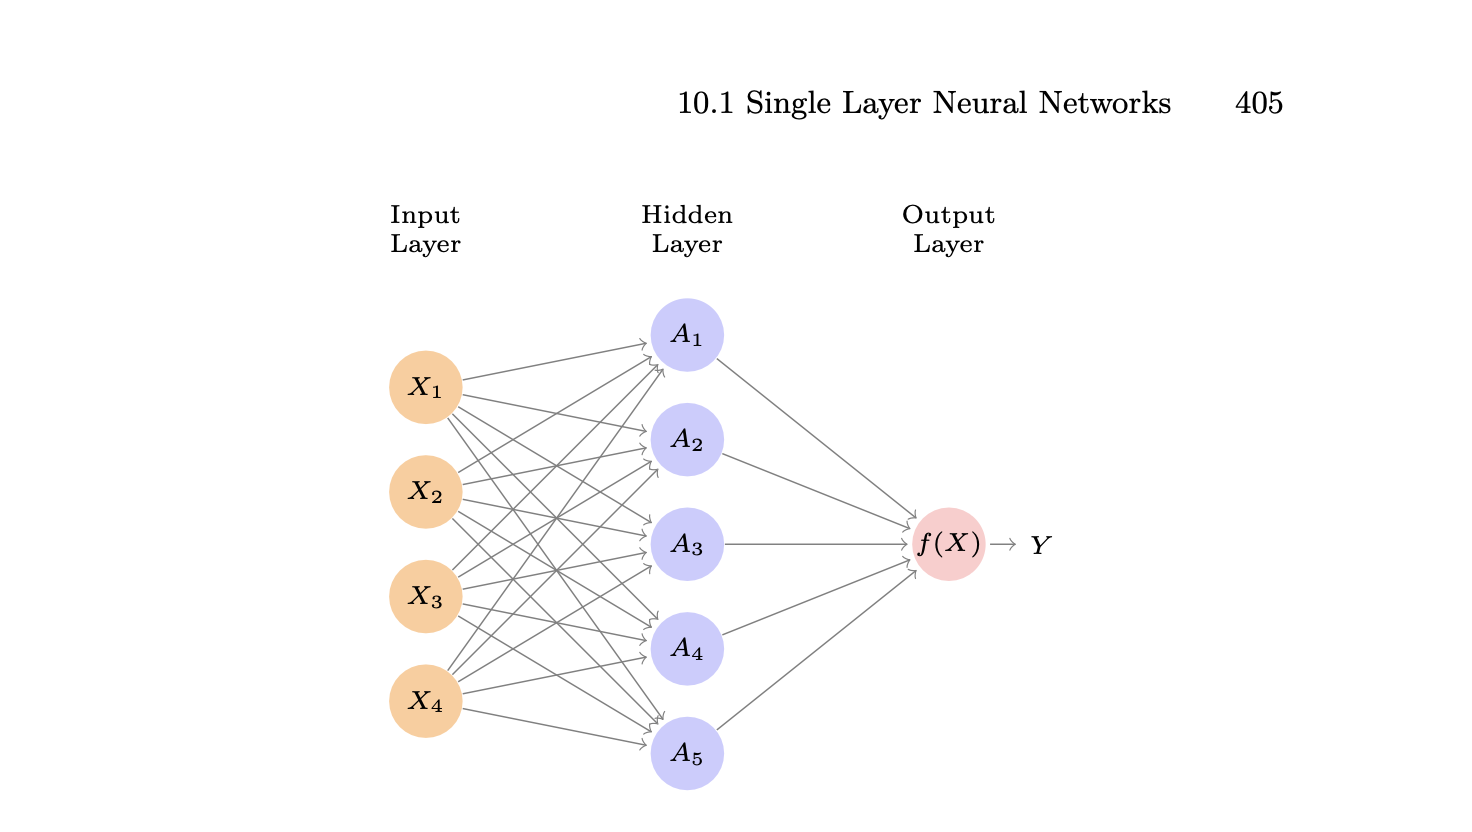
\includegraphics[width=0.8\textwidth]{442_lecs/nn.png}
\caption{A visualization of \eqref{eq_NN}. The arrows between the inputs $X$ and the hidden later each represent a parameter $w_{kj}$, where the $k$ tells us which hidden layer we connect to and the $j$ tells us which input variable to connect to. Sometimes we draw an extra input layer node to represent the intercept. The arrows from the hidden layer to the prediction layer are the parameters $\beta_k$. All of these parameters must get estimated.}
\label{fig_nn}
\end{figure}

While we won't be able to fit models like the one shown in Figure~\ref{fig_nn} directly with least squares, we will be able to fit it by optimizing over a loss function: something that you all have already seen many times! So ... a neural network really isn'y all that different from a linear model! This is a very statistical perspective on neural networks.

\subsubsection{Deep learning}

The really key idea in Figure~\ref{fig_nn} is that: \textbf{linear combinations of non-linear transformations of linear combinations} can be arbitrarily complicated and wiggly! In fact, there is a theorem that says that any continuous function $f()$ can be expressed in the form \eqref{eq_NN} as long as $g()$ is non-polynomial and $K$ is big enough. Another idea, if we don't want to make $K$ huge, is to add more layers! And more levels of non-linearity! This is shown in Figure~\ref{fig_deep}, which is also taken from ISL. 

The idea of approximating really complicated functions with these networks has really taken off in the field of deep learning! Models like the one in Figure~\ref{fig_deep} have become very state of the art in image classification, computer vision, LLMs, and basically any other big-tech application that you can possibly think of. Whatever big data you see out there in the real world- it is probably making use of deep neural networks! It almost makes me feel like there is no need to teach the other methods that we have been discussing or will be discussing in this class. But only almost! Deep neural networks are not appropriate for every circumstance, and they certainly have a lot of downsides!  

\begin{figure}[h]
\centering
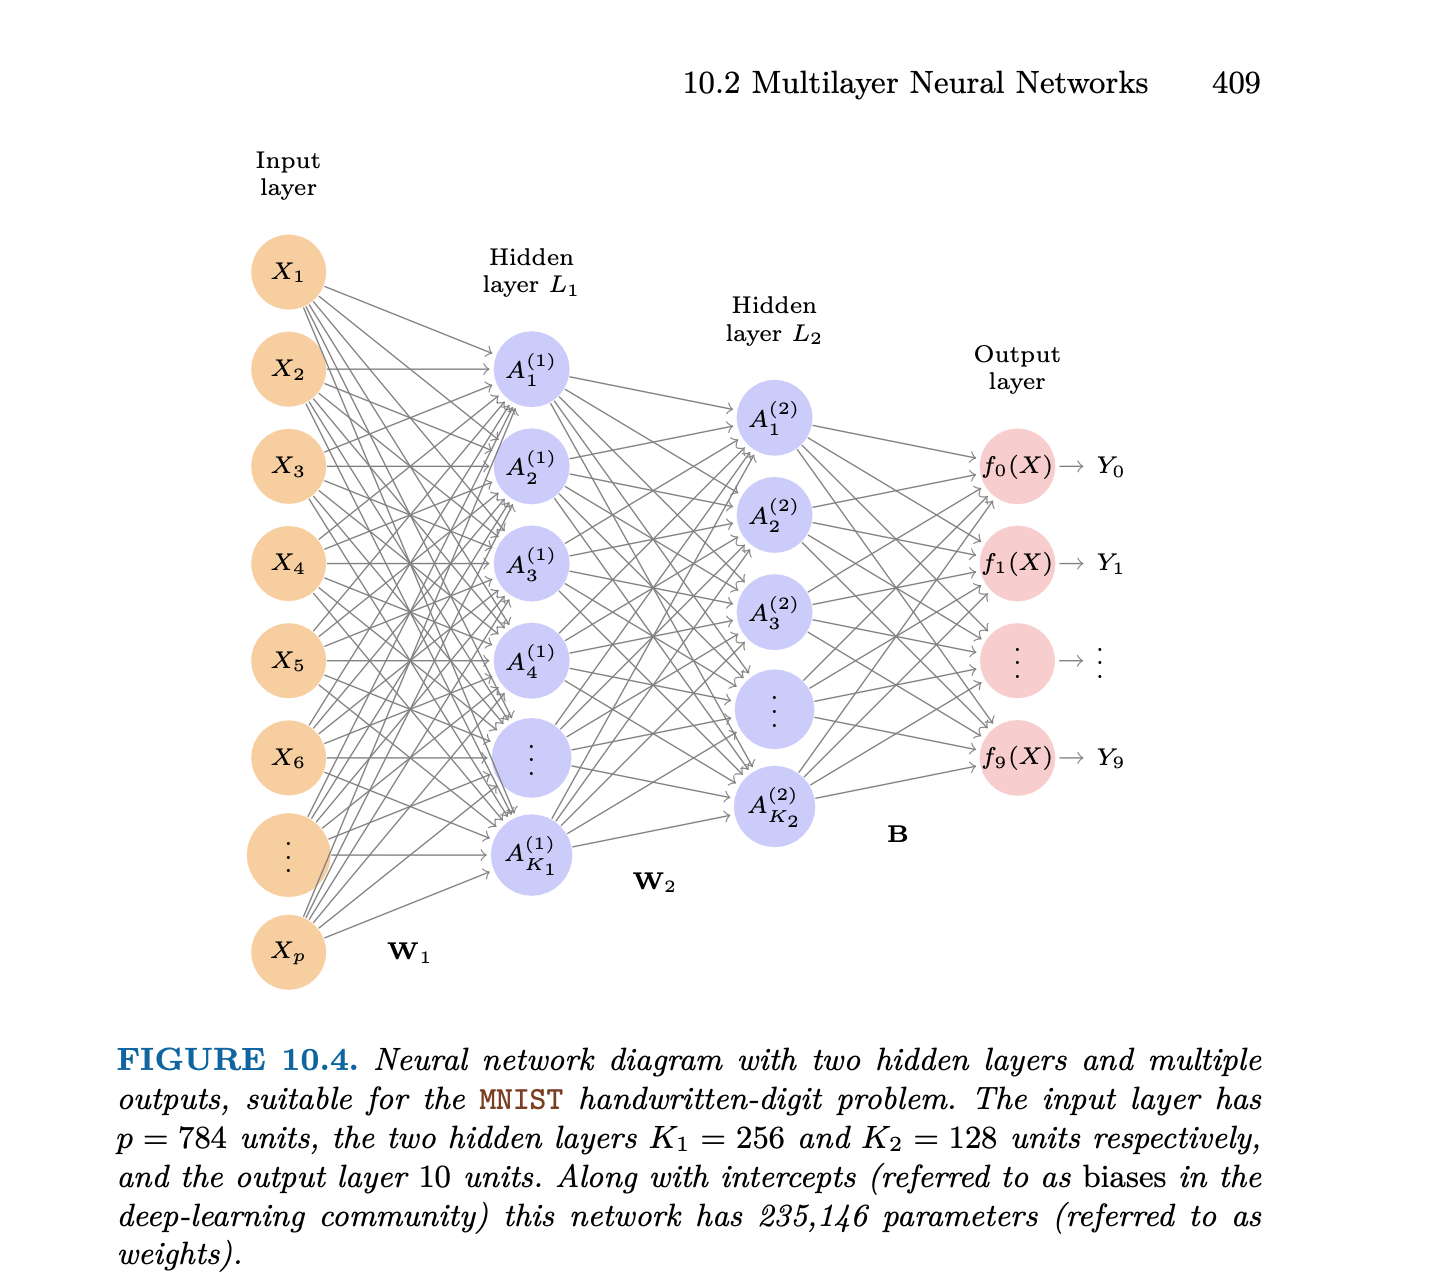
\includegraphics[width=0.8\textwidth]{442_lecs/deep.png}
\caption{A multilayer neural net. Note that here we have multiple outputs $Y$ because this is for a categorical output with 10 categories. We represent this as a vector of length 10, where $Y_k=1$ if $Y=k$ and $Y_k=0$ otherwise.}
\label{fig_deep}
\end{figure} 

\subsection{Historical context and a less statistical motivation}

When neural networks were first developed in the 1940s, there was a biological interpretation. Scientists wanted to model the living brain! An early reference is McCulloch and Pitts (1943). 

The nodes in the hidden layer are supposed to represent neurons. A neuron only fires if the amount of signal being passed into it exceeds a certain threshold. So, the activation function $g()$ was typically a step function: either the node (neuron) is turned on, or turned off. However, the step function was later replaced with differentiable alternatives for the purposes of actually fitting the model. But, the idea that the activation function should often be near 0 until it eventually gets ``activated" or ``fires" remained. 

Do you think that neural networks work well because they model the human brain (which works well), or do you think they work well because they are very expressive linear models that do automatic feature engineering? It is up to you to decide on your interpretation! I think the latter, but I also do not know much about the real human brain! 

A few more historical notes:
\begin{itemize}
\item The ideas of neural networks are so old and were developed independently by different fields!
\item But ... when did they really take off?
\item Up until 2010 or so, they were not popular in computer vision. Only Yann LeCun and Geoff Hinton were really pursuing these. After some students of Geoff Hinton won an ImageNet competition (used a neural network for an image classification task and got the best performance), then people started to pay attention.
\item By the way, my history	 knowledge was really rusty and anecdotal. I found this slide deck from a course at Univ. Wisconsin \url{https://sebastianraschka.com/pdf/lecture-notes/stat479ss19/L02_dl-history_slides.pdf} and I liked the way the material was presented: he has screenshots from a lot of cool books. Check these out and check out the related sources if you want to know more!
\item Things I learned: the ReLU activation function was an idea of Hinton+coauthor, and it was in 2010. And this change in activation function must have been a huge difference maker! 
\item You can also check out Section 1.2 of the free deep learning book: \url{https://www.deeplearningbook.org}. 
\end{itemize}



\subsection{What do I pick for my activation function $g()$?}
\begin{itemize}
\item In projection pursuit regression, the idea was that this could be a smoothing spline or something! But projection pursuit regression was always going to have like $K=5$ and one hidden layer. If we want to do BIG neural networks, we need something simple. And hopefully differentiable, because we will fit with gradient descent. 
\item From the ``neurons in the brain" view of neural networks, a 0/1 step function made sense. A neuron is either turned on or turned off. But, since a step function is not differentiable, the sigmoid/logistic: $g(z) = \frac{1}{1+e^{-z}}$ was a nice alternative. Or tanh. 
\item But, nowadays, a really common one is: $g(z) = max(0,z)$. This is called the ReLU. This keeps the motivation of a neuron being ``turned on" vs. ``turned off," but now allows really strong signals to be carried forward by having larger magnitude. One issue with this activation function is the ``dead ReLU" problem, which we will discuss. 
\end{itemize}





\subsection{Themes}

People have the tendency to treat neural networks and deep learning as magical! I hope to convince you that these are not magical, and that they in fact relate to many things that you have already seen in this class: e.g. feature engineering, basis expansion. And I hope you can start to see how neural networks relate a bit to what I talked about on the very first day of class: the biggest difference between modern machine learning and classical statistics has to do with ``how much is pre-specified". Neural network relates to feature engineering or basis expansions, but the form of the new features or the basis functions was not pre-specified.

Because NNs are not so different than everything else we can see in this class, we can discuss our favorite themes. 
\begin{itemize}
\item Bias:
\begin{itemize}
\item  We can approximate ANY continuous function $f$ with a neural network with one hidden layer and a non-polynomial activation function. We might need a really huge (but finite) value of $K$. But still! This is so cool. It means that we are not limited by modeling assumptions for a neural network: we should be able to model any true $f$ really well.
\item One note: this theorem	 says that any continuous function $f$ can be expressed using a picture like Figure~\ref{fig_nn} and certain values of the weights. It does not say that we will be able to estimate the weights from our training data! 
\item But still. Neural networks have really low bias! No bias if we use enough layers or nodes. 
\item They work really well!
\end{itemize}
\item Variance
\begin{itemize}
\item We know that variance depends on degrees of freedom, which is the effective number of parameters that we are estimating. If we make a lot of hidden layers, or if we make $K$ really big, then surely we will have more parameters than we do training observations $n$. Isn't this really bad for variance? Won't we memorize our training set and overfit?
\item Short answer: statisticians were very skeptical of deep learning for these reasons for many years. Over-parameterized models should score poorly for variance! And they definitely do when you don't have a really big value of $n$. 
\item We should regularize to help keep the variance under control. More on this when we discuss double descent! We should use a validation set to stop training before we overfit.
\item But sometimes, when you have enough data, NNs perform really well on test sets, even though they are over-parameterized. This also isn't magic: we need to distinguish between number of parameters and number of effective parameters
\end{itemize}
\item Interpretability
\begin{itemize}
\item This is our first true black-box model. It is really hard to understand where the predictions of a neural network model are coming from!
\item Do not pick deep learning if you have a scientific application where you need to interpret and explain your results!
\item Since the model itself is a black-box, we will need to use clever explainability techniques on top of the model to try to understand what is going on: this is a hot area of research that we will discuss after spring break.  
\end{itemize}
\item Usability (is the method ``off the shelf")?
\begin{itemize}
\item Neural networks tend to require a lot more tuning than something like a random forest. They are NOT very ``off-the-shelf". This is a reason why they took a while to become popular. They were hiding in the background for many years before deep learning really took off. 
 \item Evidence: I will not make you do a HW problem where you actually use neural nets, because the R packages are finicky! 
\item There is flexibility, which is nice: you can modify the architecture really to your liking. If you know what you are doing, this is great! But this flexibility does make it harder to make all-purpose, useable software. 
\end{itemize}
\item Computational efficiency	
\begin{itemize}
\item We are going to actually go over gradient descent and backpropogation on Thursday! So you will learn more about fitting. 
\item We need to use a slow iterative algorithm to fit: and we always need to be worried that maybe we did not converge in our fitting! 
\item However, there is also something very parallel and distributed about our computations, which makes huge deep neural networks actually feasible to fit. 
\end{itemize}
\end{itemize}





\section{Thursday, March 6: Fitting a neural network: backpropagation and gradient descent}

Given our neural network architecture and our training data, we need a way to FIT the network. This means coming up with values for all of the $w$s and all of the $\beta$s. These should be chosen to give us good predictive accuracy on the training set (although we also want to be careful of overfitting). We will fit a neural network with gradient descent (a very general technique). They key insight for neural networks is that we can use the chain rule to do gradient descent in a very organized way, called backpropagation. 

\subsection{Gradient descent}

Let $\theta$ be a really long vector that denotes our current set of parameters (values for every line in our neural network picture). Recall that $\theta$ consists of $w$s and $\beta$s, where $w$s operate between the inputs and the hidden layers, and $\beta$s act on the activation layer to give us the output. 

Given $\theta$, we can send an input example $X_i$ ``forward" through the network. This gives us a prediction $\hat{Y}_i$. 

Since this is a training example, we can then compute the loss: $(Y_i - \hat{Y}_i)^2$. 

If we do this over the whole training set, we get the overall loss for this current value of $\theta$:
$$
L(\theta) = \sum_{i=1}^n (Y_i - \hat{Y}_i)^2.
$$

Whenever we have a loss function that we want to optimize with respect to $\theta$, we wish we could take the derivative and set it equal to $0$. Here, there is no way we will be able to solve for that in closed form!

Instead, let's take steps along the negative gradient (with respect to $\theta$) of the loss function. The gradient of $L(\theta)$ with respect to $\theta$ is denoted $\nabla L(\cdot)$. The gradient is simply the vector of partial derivatives with respect to each element of $\theta$.  

We want to take steps in the direction of the negative gradient of the loss function so that we always move a current guess $\theta^t$ to a new guess $\theta^{t+1}$ in a way that will make the loss smaller the next time we compute it. What a nice idea!

While we take a step in the ``direction" of the gradient, we don't want to take a step that is the SIZE of the gradient. We want to take really small steps so that we don't ``overshoot" a minimum. So we let: 
$$
\theta^{t+1} = \theta^t - \rho \nabla L(\theta^{t}),
$$
where $\rho$ is a small learning rate that we get to pick.

Note: if our step size $\rho$ is going to be approximately the same for all elements of $\theta$, we probably want the elements of $\theta$ to all be in the same ``units". This means that we probably want to normalize our input variables $X$! This is not changed from other algorithms. 

We keep taking small steps in the direction of the negative gradient until our ``guesses" stop changing. At this point, we have landed in a region of $\theta$-space where the derivative is 0! This hopefully means that we found a minimum of the loss function!

Unfortunately, there is no guarantee that it is a global minimum. For really complicated non-convex loss functions, we can get stuck in suboptimal local minima. We will discuss strategies for avoid it later! For now, see Figure~\ref{fig_gd} for an illustration of gradient descent in a setting where $\theta$ is one-dimensional. 

Gradient descent is a really general optimization technique! It is used in contexts that have nothing to do with fitting neural networks!

\begin{figure}[h]
\centering 
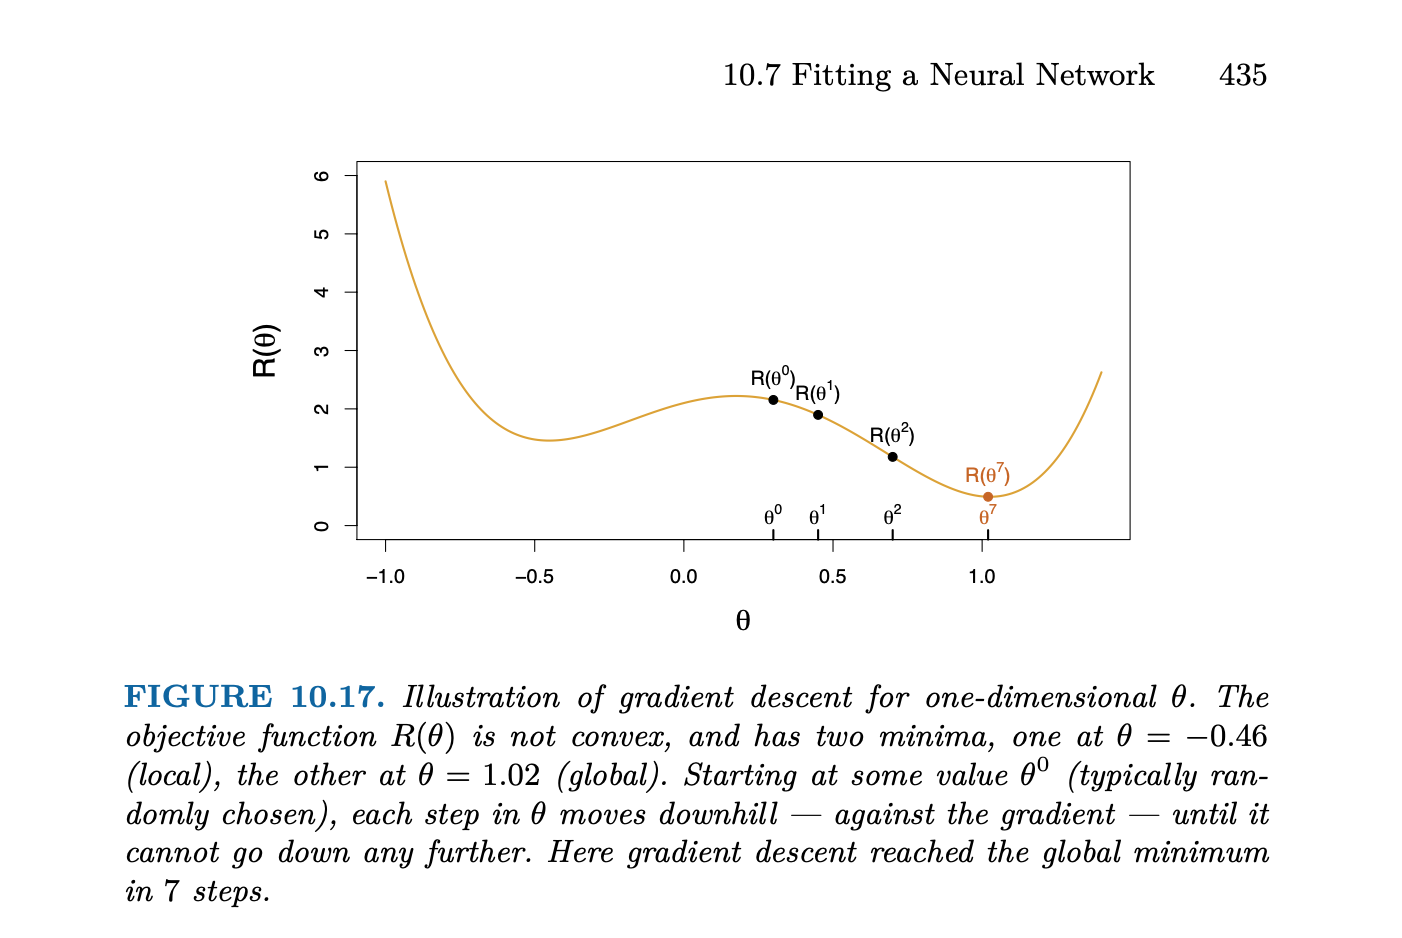
\includegraphics[width=0.7\textwidth]{442_lecs/gradient.png}
\caption{An illustration from ISL of gradient descent for a very simple one-dimensional $\theta$. In this case, we found the global minimum. But that is not guaranteed!}
\label{fig_gd}
\end{figure}

\subsection{Backpropagation and the Chain Rule}

Let's study gradient descent for a one-layer feed-forward neural network in the following very simple case. This is a network with one hidden later and three hidden nodes ($K=3)$. There are also only three inputs ($p=3$). For simplicity, I did not draw the intercept (bias) terms only the diagram.

\begin{center}
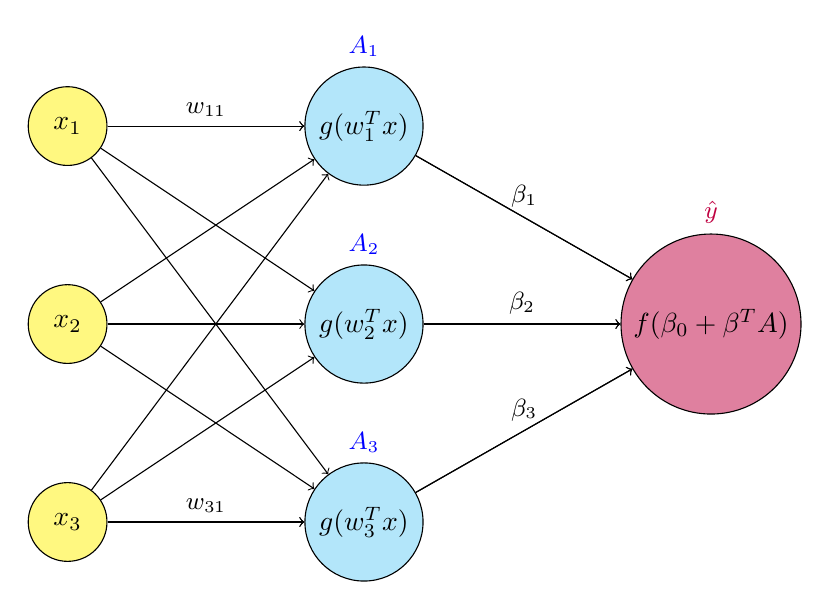
\begin{tikzpicture}[
    node distance=1.5cm and 2.5cm,
    neuron/.style={circle, draw, minimum size=1cm},
    every label/.style={font=\small}
]

% Input layer
\node[neuron, fill=yellow!50] (I1) {$x_1$};
\node[neuron, fill=yellow!50, below=of I1] (I2) {$x_2$};
\node[neuron, fill=yellow!50, below=of I2] (I3) {$x_3$};

% Hidden layer
\node[neuron, fill=cyan!30, right=of I1, label=above:\textcolor{blue}{$A_1$}] (H1) {$g(w_1^T x)$};
\node[neuron, fill=cyan!30, right=of I2, label=above:\textcolor{blue}{$A_2$}] (H2) {$g(w_2^T x)$};
\node[neuron, fill=cyan!30, right=of I3, label=above:\textcolor{blue}{$A_3$}] (H3) {$g(w_3^T x)$};

% Output layer
\node[neuron, fill=purple!50, right=of H2, label=above:\textcolor{purple}{$\hat{y}$}] (O) {$f(\beta_0 + \beta^T A)$};

% Connections (Input to Hidden)
\foreach \i in {I1, I2, I3}
    \foreach \h in {H1, H2, H3}
        \draw[->] (\i) -- (\h);

% Connections (Hidden to Output)
\foreach \h in {H1, H2, H3}
    \draw[->] (\h) -- (O);

% Label the specific weights
\draw[->] (I1) -- node[above] {\small $w_{11}$} (H1);
\draw[->] (I3) -- node[above] {\small $w_{31}$} (H3);
\draw[->] (H1) -- node[above] {\small $\beta_1$} (O);
\draw[->] (H2) -- node[above] {\small $\beta_2$} (O);
\draw[->] (H3) -- node[above] {\small $\beta_3$} (O);
\end{tikzpicture}
\end{center}

In this case, suppose that we are doing regression, and so the function $f()$ at the very end is just the identity function. Recall that when we are doing classification, we need to turn our final output into a probability or a prediction using a link function. But for regression we are all set on our original scale. 

For given values of $w_{10},\ldots, w_{pK}$ and $\beta_0,\ldots, \beta_K$, each input example $x_i$ gets turned into a $\hat{y}_i$. Our squared error loss for our training set is: 
\begin{align*}
L(\theta) &= \sum_{i=1}^n L_i(\theta) = \sum_{i=1}^n (y_i - \hat{y}_i)^2 \\
&= \sum_{i=1}^n \left( y_i - \beta_0 - \sum_{k=1}^3 \beta_k A_k \right)^2 \\
&= \sum_{i=1}^n \left( y_i - \beta_0 - \sum_{k=1}^3 \beta_k g \left(w_{k0} + \sum_{j=1}^p w_{kj} x_{ij}\right)\right)^2. 
\end{align*}

I wrote this at multiple levels of granularity. Sometimes it is nice to explicitly see that the loss function depends on every $w$ and every $\beta$. Other times, it is kind of nice to hide this detail. 

Suppose that we begin with random guesses for every $\beta$ and every $w$. Then, we send our entire training set ``forward" through the neural network and compute this loss function given the current predictions. Then, we compute the gradient. We step along the gradient, and we update our guesses of $w$ and $\beta$ accordingly. 

For our neural network loss function, let's figure out the steps along the gradient. The key idea is that we can chain rule! 

In this example, since $f()$ is just the identity function, we have that:
\begin{align*}
\frac{dL}{d \beta_k} &= -2 \sum_{i=1}^n (y_i - \hat{y}_i) \frac{d\hat{y}_i}{d \beta_k} \\
&= - 2 \sum_{i=1}^n (y_i - \hat{y}_i) A_k \\
&= -2 \sum_{i=1}^n (y_i - \hat{y}_i) g \left(w_{k0} + \sum_{j=1}^p w_{kj} x_{ij}\right) 
\end{align*}
And then:
\begin{align*}
\frac{dL}{d w_{kj}} &= -2 \sum_{i=1}^n (y_i - \hat{y}_i) \frac{d\hat{y}_i}{d w_{kj}} \\
&= -2 \sum_{i=1}^n (y_i - \hat{y}_i ) \beta_{k} g' \left(w_{k0} + \sum_{j=1}^p w_{kj} x_{ij}\right) x_{ij},
\end{align*}
where the specific form depends on the activation function $g()$. But hopefully we choose a differentiable $g()$ where this isn't too complicated.

Note that both of these partial derivatives imply that the direction of our step depends on our residuals $y_i - \hat{y}_i$: this is a good thing! We want to make the residuals smaller! 

The reason that we call this special version of gradient descent ``backpropagation" is that we can think of these applications of the chain rule as stepping backward through our network, and passing our residuals/errors along as we go. As we add more layers to the network, we add more chain rules! But nothing gets too difficult. 

Recall that gradient descent lets:
$$
\theta^{t+1} = \theta^t - \rho \nabla L (\theta^{t}).
$$
So, the size of the step depends on the learning rate $\rho$, the size of the residuals $(y_i - \hat{y}_i)$, the magnitude of the gradient evaluated at $\theta^{t}$, and the actual inputs $x_{ij}$. This is a lot of things! Making sure that we take the right sized steps can be very finicky. 

\subsection{Stochastic Gradient Descent}

Instead of computing the loss function and the gradient over all $n$ training instances at once, we typically go instance-by-instance or batch-by-batch. This is related to \emph{online learning}, which you read about for HW2. A batch is just a subset of the $n$ training observations. The motivation is that we will speed up our learning about $\theta$ by updating $\theta^{t}$ more often. If our training set is huge, we don't want to bother processing a massive training set with a bad guess $\theta^{t}$. We should take advantage of the fact that we see a lot of errors in the first few training examples, and we should update $\theta^{t}$ to $\theta^{t+1}$ right away. 

This is stochastic because our gradient computed on a small number of training observations should be a good approximation of our overall gradient. But the exact step we take depends on the specific training observation! VERY STRANGELY: It turns out that stochastic gradient descent enforces its own form of approximately quadratic regularization. We will come back to this! So there is something really important about the relationship between stochastic gradient descent and overfitting, that wasn't necessarily the original motivation for SGD. 

It also turns out that the extra noise added with SGD can help us avoid local minima! That is cool too! We bounce around $\theta$-space and explore a bit more. 

If we are using SGD and we end up iterating through the entire training set 10 times, this means that we used 10 epochs. But, this might mean that we used $T=100$ updates of $\theta$, if our batch size was 1/10 of the training set. 

\subsection{Complications}

While (stochastic) gradient descent is a very general idea that can be used in many contexts, it is ultimately only a way to find an approximate minimizer of a loss function. There are a lot of complications.

We need to choose our step size and our initial guesses for the parameters. We also need to be worried about our initial starting conditions; as these can determine whether or not we get stuck in a local minimum. With bad initial weights (too large), we can have vanishing gradients, and we will think we have converged right away, without ever updating our initial weights. Or, with a ReLU activation function, it is the case that a certain unit is never ``turned on" for the training set given the initial weights, it will actually NEVER get turned on. It is a permanently dead Neuron. All of this is bad! Maybe I will put one of these on your HW. 

We also need to know how big of a batch we should use for SGD. 

We need to know how many iterations or epochs to train for. In theory, I guess we should go until the $\theta^t$ stop changing (convergence). But ... what if we have used up all of our computational resources and we have not yet converged? 

All of these things ACTUALLY affect our fit. Fitting a neural network can be so finicky in practice, unless you have a lot of resources and are an expert. This makes them a bit less usable or ``off-the-shelf" than some alternatives. 

We also need to decide on a model architecture before we start. How many hidden nodes do we want? How many hidden layers? What activation function should we use? Etc. 

\subsection{Overfitting and model complexity}

We know that a neural network model with $K$ hidden units in one layer and $p$ inputs needs to learn around $(p+1)*(K+1)$ parameters. If we add more hidden laters, this just gets bigger.

We know that, if we have $n$ training datapoints, a model with more than $n$ parameters should be able to memorize the training set. And we know that this is bad, because we will overfit, and will have poor generalization error. 

In modern deep neural networks, we often have more parameters than datapoints! So, how can we prevent overfitting?

There are several strategies that people were already doing:
\begin{itemize}
\item Add explicit regularization to our loss function! Like $\lambda$ times the L1 or L2 norm of our $w$s and our $\beta$s. This affects every step of our gradient descent calculation, and could make it more complicated. But it will keep the variance of our model down, as we know. 
\item Random dropout: A possibly simpler version of regularization. We can just randomly turn off some hidden nodes when we pass some training observations through the network. This forces other nodes to pick up the slack of these turned-off nodes. This means that a single node cannot be used to memorize a single training point---- because it has to perform multiple tasks. What a super cool idea!  
\item Early stopping via a validation set. Suppose that we want to encourage our weights to be small. We can start with small initial values. Then, every time we finish a batch or an epoch, we can check our error on a validation set. Presumably at first, this will be decreasing as we update our weights. If, at some point it starts increasing, we can assume that we started overfitting, and we can just stop training (even if we haven't converged). This is cool and should also work well! 
\end{itemize}
Note that any type of regularization adds to our training complications. How to we pick our penalty parameter? How do we pick how much dropout to have, or how MUCH the validation error needs to increase in order for us to think we should stop? There is already so much going on! This is not automated! 

Ok, but even with all of these strategies, don't we think that these massive models will overfit? And perform badly in terms of the bias-variance tradeoff? Especially when we don't have that many training observations? 
\begin{itemize}
\item Mostly, yes I do think this!
\item But empirically, we have seen a strange phenomenon called double descent.
\item It turns out it is not actually that strange or mysterious! Let's explore. 	
\end{itemize}


\subsection{Double descent, and its relation to stochastic gradient descent}

This is one of my favorite topics! See ISL 10.8 for a beautiful explanation. You will also explore this concept on your homework, and I may fill in these notes in more detail after Thursday's class. 

The story of double descent is shown in Figure~\ref{fig_dd}. 

\begin{figure}
\centering 
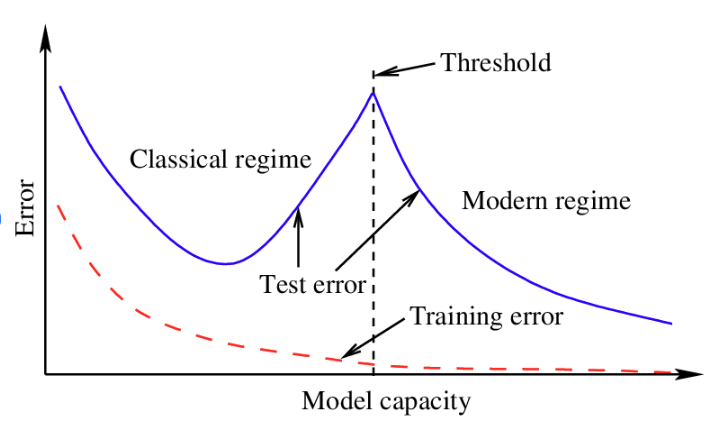
\includegraphics[width=0.6\textwidth]{442_lecs/dd.png}
\caption{A classic illustration of double descent.}	
\label{fig_dd}
\end{figure}





\subsection{Extensions of neural networks}

We have barely scratched the surface. There are so many cool topics we could cover. Such as multitask learning, auto-encoders, convolutional neural networks, or recurrent neural networks. Auto-encoders also relate to semi-supervised learning. We are not going to cover these! But hopefully you now have a little bit of foundational knowledge to understand these better in the future. And you could always do one of these for your final project!





\section{Monday, March 10: Classification and Regression Trees}

This is one of my favorite topics! At first, this algorithm might seem like a totally ``new idea". But later, I hope you will see a lot of connections with algorithms we have already studied!

One note before we start: there are actually a lot of algorithms out there for building classification and regression trees! I will get to this in ``historical context." Whenever I don't say otherwise, if I am talking about a tree algorithm, assume that I am talking about the CART framework, which was popularized by Breiman et al. in 1984. 

\subsection{The main idea of the algorithm}

Let's start with some really basic motivation for a regression tree. At first glance, it might seem a bit different than the other methods we have seen in this class. 

The motivation begins with the left panel of Figure~\ref{fig_cart}. We have two covariates, $X_1$ and $X_2$. And then we have a numerical response variable $Y$. We begin the algorithm with the simplest possible model. This model just ignores the covariates and predicts $\hat{y} = \bar{y}$ for all observations. In this case, $\bar{y} = -2.6$. This is the ``intercept only" model. It has MSE given by: $\sum_{i=1}^n (y_i - \bar{y})^2$.

The algorithm then proceeds in a way that might remind you of forward stepwise regression. The algorithm says: at this moment in time, what is the binary split in my covariate space that will most improve the MSE, if I now let each sub-region be summarized by its own sample mean. This is illustrated in the second panel of Figure~\ref{fig_cart}. In this particular dataset, it turns out that the best way to chop our space into two is to draw a vertical line at $X_1 = -0.89$. Once we do this, any observation to the left of the split gets $\hat{y}=10$, and every observation to the right of the split gets $\hat{y}=-7$. This cutoff of $X_1 = -0.89$ was chosen greedily after considering all possible splits.

Let's write this down more rigorously. As of step 1 in the algorithm, our model has a single ``region" in it. This region is $R_0 = \mathbb{R}^p$: the whole covariate space. The set of possible splits are indexed by $j \in 1,\ldots,p$ and $s \in 1,\ldots, n$, where $x_{j,(s)}$ denotes the $s$th order statistic of the $j$th covariate\footnote{In the case of non-ordinal categorical $X_j$, we assign orders to the categories by sorting them by their average value of $Y$ in the training set. Thus, the order statistics are still defined; we just have a lot of ties in the order statistics: meaning that $x_{j,(1)}=x_{j,(2)}=x_{j,(3)}$ if all three observations belong to the same category.}. At the first level of the tree, we search exhaustively for:
\begin{equation}
\label{eq_SPLIT}
j^*, s^* = \argmax_{j \in 1,\ldots,p, s \in 1,\ldots n} Gain(R_0, j,s) = \sum_{i \in R_0} (y_i - \bar{y}_{R_0})^2 - \left( \sum_{i \in R_{L(j,s)}} (y_i - \bar{y}_{R_{L(j,s)}})^2  + \sum_{i \in R_{R(j,s)}} (y_i - \bar{y}_{R_{R(j,s)}})^2 \right),
\end{equation}
where $R_{L(j,s)} = \{ i \in R_0 : x_{j,i} \leq x_{j,(s)}\}$ and $R_{R(j,s)} = \{ i \in R_0 : x_{j,i} > x_{j,(s)}\}$. We refer to these as the regions to the left and the right of the split. Note also that $\bar{y}_R = \frac{1}{|i \in R|} \sum_{i \in R} y_i$ just denotes the sample mean of $y$ within a certain region. This was a lot of notation, but it can be worth it to make sure that you really understand what the algorithm is doing! But the idea is simple: we choose the split that most improves the MSE of our model right now. Alternate Gain functions are possible, but this MSE one is the one used by Breiman et al. (1984) in their very widely used CART algorithm. 

\begin{figure}[h]
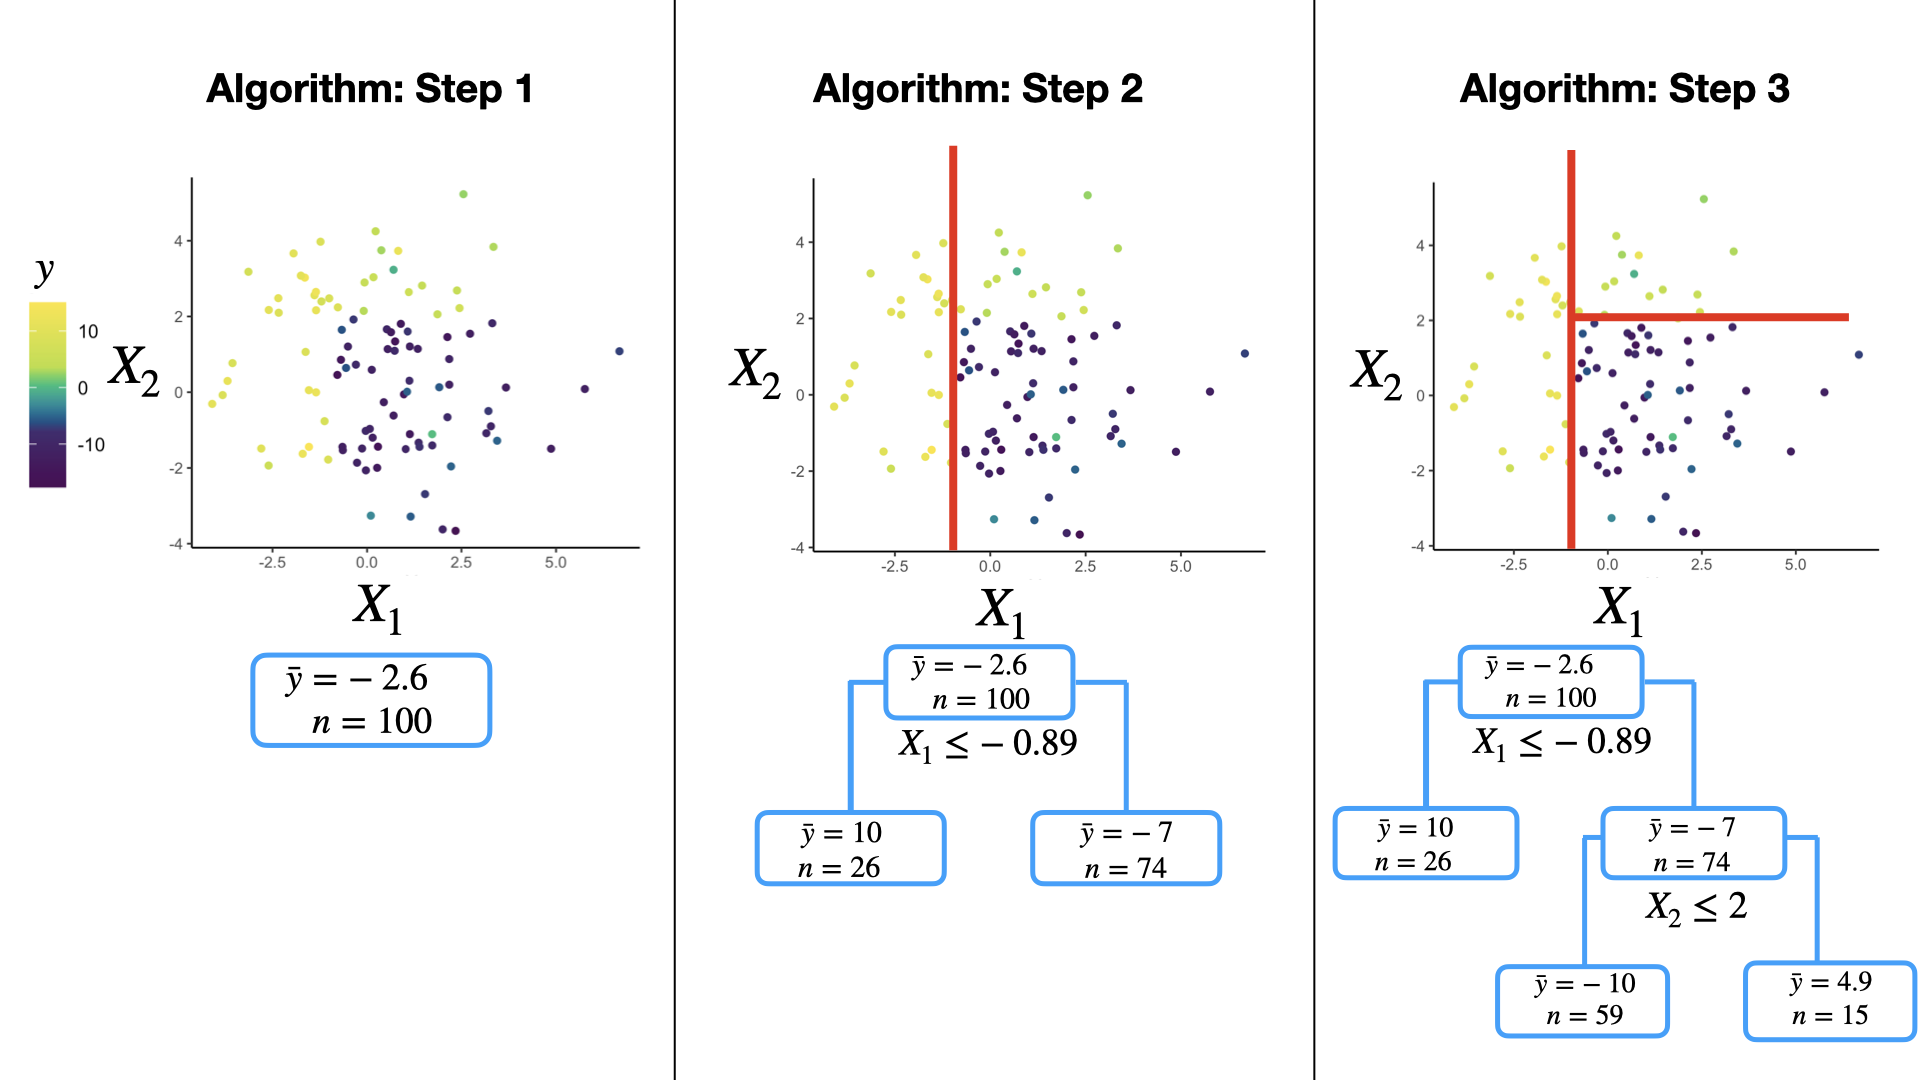
\includegraphics[width=0.9\textwidth]{442_lecs/CART_figure/CART_figure.001.png}
\caption{A little animation of the first three steps of a regression tree algorithm. Here, we have two covariates: $X_1$ and $X_2$. And then we have a numerical response variable $Y$. In this case, it seems like the data is generated from a ``true tree" structure, where there are rectangles in covariance space that define the average value of $Y$. The CART algorithm uses binary recursive partitioning to greedily search for the best possible rectangles, according to MSE!}	
\label{fig_cart}
\end{figure}

Finally, the right panel of Figure~\ref{fig_cart} shows what happens next. Regression trees are \emph{recursive partitioning algorithms}. So, the greedy search for the best possible splits, but now $R_0$ is replaced by the already-selected regions $R_{L(j^*,s^*)}$ and $R_{R(j^*,s^*)}$. We proceed until a stopping criteria is met.

The final model is a set of nested rectangles in covariate space. The prediction in each rectangle is just the sample mean of the training observations in that rectangle. We draw the model as a tree; as shown in Figure~\ref{fig_cart}. We write this model as:
$$
\hat{y} = \hat{f}(X) = \sum_{R \in \mathrm{TREE}} \bar{y}_R \bold{1}\{X \in R\}. 
$$
Sometimes the final regions in the tree are called leafs, and the series of splits that lead to them are called branches. This really leans into the tree analogy. I will just as often refer to them as terminal regions or terminal nodes, etc. 

We really have now gone over the main idea of trees! Now we will talk about some considerations and extensions. 

\subsection{Considerations, extensions, and historical context}

\subsubsection{Stopping criteria}

How do we know how big to build our tree? As you may have guessed, this is the main knob that controls our bias-variance tradeoff for trees. 

The biggest possible tree would keep splitting until we have one training observation per leaf region. This tree would have worst-case depth $n$, but likely depth closer to $log(n)$ if the tree remains more balanced. I think you all know that a tree like this will overfit severely to the training data, and we probably do not want to build this tree! We should stop before this! 

Some simple ideas for when to stop are to pre-specify the maximum depth of our tree, or the minimum node size in our tree (i.e. stop splitting when the region has less than 10 training observations in it). However, these are stopping criteria that do not adapt to the amount of signal in the data. The true ``right-sized" tree probably depends on the signal in our data! So, there are some more popular choices. 

Consider \eqref{eq_SPLIT}. What if we decided to not choose ANY split if this gain does not exceed some threshold? For example, if the MSE does not improve by more than 5\% when pick the best possible way to split this region, do not split this region at all. Such an idea is very similar to doing forward stepwise selection with an AIC or BIC stopping criteria. We recognize that ANY split will improve the training MSE *some*, but we want to make sure that the split seems ``worth it". In the \texttt{rpart} R package, this is controlled by the parameter \texttt{cp}. From the \texttt{rpart} documentation: ``any split that does not decrease the overall lack of fit by a factor of \texttt{cp} is not attempted. For instance, with anova splitting, this means that the overall R-squared must increase by \texttt{cp} at each step. The main role of this parameter is to save computing time by avoiding splits that are obviously not worthwhile." The default in \texttt{rpart} is 0.01, which is pretty small. This is an example of an \emph{adaptive stopping criteria}. 

Your textbook (ISL) calls the adaptive stopping approach above ``short-sided". The idea is that, due to the greedy nature of CART, it could be the case that no split will exceed the MSE threshold ``right now", but it could help us uncover an important interaction in the next level of the tree. So, it would be good to avoid stopping too early! 

Another idea is to grow a tree that is purposely too large, and then to \texttt{prune} splits away from the tree. More formally, let:
$$
L_\lambda(T) = \sum_{R \in T} \sum_{i \in R} (y_i - \bar{y}_R)^2 + \lambda |T|.
$$
This is a loss function that incorporates both tree MSE as well as a penalty term that penalizes larger trees: $|T|$ denotes the number of leaves in a tree. It turns out that nice properties of trees tell us that, if we start by building a large tree $T^{big}$, then there is a simple nested sequence of sub-trees that corresponds to the best tree for different values of $\lambda$. And we can find this sequence of trees easily: starting from $T^{big}$ we prune the ``weakest link" in the tree one at a time. This gives us the nested sequence of trees. This is a ``solution path"- like we had for Ridge or Lasso.  

To be really complete, we would want to use cross-validation to pick the best value of $\lambda$. And then we would want to re-fit a tree to the full training set using this value of $\lambda$. If you are not yet comfortable with the idea of cross validation + refitting to entire training set, please ask questions before the midterm! It is an important idea! 

\subsubsection{Categorical predictors}

CART can really seamlessly handle categorical predictors. We don't need to turn them into dummy variables!

The Breiman et al. CART algorithm always makes BINARY splits; even for categorical variables. You might encounter other decision tree algorithms some day that would make a three-legged-split for a categorical variable with three categories.

Ordinal categorical variables still have order statistics, so we split in the same manner than we did above in \eqref{eq_SPLIT}. For unordered categorical variables with $k$ categories, we do not need to consider $2^k$ possible ways to split the variable into two groups. We just order the categories by $\bar{y}$ on the training set, and then only let ourselves make a binary split that respects the ordering of these categories. 


NOTE: some critics of CART do not like the following fact. A numerical covariate has $O(n)$ chances to be chosen as the winning split. A binary categorical covariate has only 1 chance to be chosen as the winning split! If the binary covariate is truly important, but is associated with the numerical one, the numerical one will often appear in our tree! Just due to the extra random chance that it gets to be selected as a winner. This is too bad! There are modifications to the algorithm that try to get around this bias. 

\subsubsection{Categorical response}

CART is really easily used for either regression or classification.

For classification trees, all we do is modify our gain function. Instead of using MSE,  we split based on either Gini Index or Entropy. With either of these, we are choosing a split that makes the resulting child notes as pure as possible: meaning homogenous with respect to $y$. 

While we use Gini Index or Entropy to choose our splits greedily, we might still do cross validation using simple 0/1 classification error loss. 

\subsubsection{History}

I got some nice historical notes from this paper: \url{https://pages.stat.wisc.edu/~loh/treeprogs/guide/LohISI14.pdf}. 

The first classification tree algorithm was in 1963, and it was published under the name ``automatic interaction detection (AID)". This should already tell you something about why trees have been so popular- people absolutely love this feature that they can identify interactions without those interactions being pre-specified. At first, AID did not attract much attention from statisticians. People were worried about overfitting. People were also worried that, in the presence of correlated predictors, the conclusions could be spurious. Probably only one of the pair of correlated predictors will be selected for the tree, and the other will be totally left out. It might be dangerous to over-interpret the tree as signaling variable importance in that case\footnote{I agree!}. At the same time, however, computer scientists were making their own decision trees for ``concept learning." It seems that an early reference is Hunt, Marin, and Stone (1966). The algorithm that I learned about in CS class is ID3, which was published by Quinlan in a series of work in the 1980s. This is again a setting where great ideas were coming out concurrently in multiple disciplines!

The credit for ``popularizing" trees, at least in statistics, goes to Breiman et al. in 1984. I am pretty sure that one of the main innovations by Breiman et al. that really helped people take up trees was the introduction of efficient cost-complexity pruning. 

Since trees first became popular, there has been a lot more work on them! Some statisticians (including me) do not like that the splits in a CART tree lack a notion of statistical significance\footnote{This is very related to my claim, which we never finished going over, that you cannot easily do inference after stepwise regression. Greedily searching for optimal things makes inference hard.} One family of competing algorithms is called CTree; splits are chosen based on statistical significance, rather than based on an improvement in MSE. There are also models that make splits on linear combinations of variables, instead of single variables. Or models that fit an entire regression model to each leaf node, rather than choosing a piecewise constant model. And I am sure I am missing a lot of innovations! 

\subsection{What do we think about trees?}


\subsubsection{Bias}

An extremely large tree has almost no bias. We can approximate basically any function with a big combination of step functions. So if $n$ is big and our tree is big, trees are flexible. It is nice that trees can capture interactions between variables and other sorts of non-linear relationships without us needing to pre-specify.

However, a tree of reasonable size is very limited. Consider the case where $Y = 5 * X_1$. To approximate this well by a sequence of binary splits on the variable $X_1$, we will need a lot of splits! As we add more and more, our approximation will get better and better! But this function will obviously be much easier to approximate with a linear model!

In general, if the true data generating mechanism is not made up of rectangles in covariate space, a simple tree might struggle. But, if you are worried that rectangles in covariate space are REALLY biased, not that a really big tree works a lot like 1-NN, which we know does not have bias. See below for more about the connection to KNN. 

\subsubsection{Variance}

An extremely large tree has a lot of variance because it overfits. But even a small tree can have a lot of variance due to the greedy nature of trees. A small change to the input dataset can totally chance our first split, which could then affect our whole tree- especially if we only plan to make a small tree. So trees do not score super well for variance.

\subsubsection{Interpretability}

Trees are a dream! We can explain our predictions so easily to non-experts! Even things like interactions do not seem scary when they are presented as a tree! However, I have some notes below about a fundamental issue. If we know that our tree is unstable (high variance), what are we really interpreting? This makes formal inference really important. Which is something I worked on in my PhD!

\subsubsection{Use-ability}

Trees are a dream! They are ``off the shelf". The only tuning parameter is tree size, and tree size is something that we understand. And the nested-tree property of the pruning algorithm makes it really nice. 

We don't need to scale our predictors or worry about whether or not we are including an intercept. Categorical predictors need not be converted to binary. Missing data is also seamless to incorporate using the concept of surrogate splits. 
You don't need to start with preprocessing of variable selection. Trees do built in variable selection, and are not TOO impacted by curse of dimensionality. 

\subsubsection{Computational Efficiency}

When I first learned about trees, I thought that the algorithm sounded slow. Search exhaustively for best possible split? But now that I know about things like neural nets, I'm less concerned haha. Trees are pretty easy to implement. The greediness saves us. $O(np)$ things to compute at each level to choose a split. At least no squared terms, right? And the tree depth will be at MOST $n$, usually more like $log(n)$ if balanced. So maybe $O(np log(n))$. This really isn't bad. The pruning algorithm is also efficient. 

\subsection{Drawing connections!}

Right now, it might seem like decision trees are a random topic we have thrown in that are totally different from the other algorithms that we have seen. This is not true! Let's draw some connections.

\subsubsection{Write as a regression model or optimization problem}

Really, a regression tree defines a model class of piecewise constant models on rectangles in covariate space. So we could just abandon the whole tree idea and say that we are looking for a set of regions $R_1,\ldots, R_T$ such that we minimize
$$
L_\lambda(T) = \sum_{r=1}^T\sum_{i \in R_r} (y_i - \bar{y}_{R_r})^2 + \lambda |T|,
$$
and where $\hat{y} = \sum_{r=1}^T \bold{1}(X \in R_r) \bar{y}_{R_r}$. 

This looks a bit more like an optimization problem or a regression problem. We are regressing onto lots and lots of possible step-function indicator variables, but we are doing variable selection first to decide which ones to include. We can think of trees in this way! And then the innovation is just that this loss function will be really really difficult to minimize exactly. So, we give up on searching fully for the optimal tree. We instead use our greedy, top-down approach. Which finds a pretty good tree, but not necessarily the very best optimal tree. This reminds us of the difference between best-subset regression, which is infeasible, and stepwise regression, which is a greedy approximation.


\subsubsection{How is a regression tree like KNN?}

At the end of the day, the prediction $\hat{y} = \hat{f}(\xte)$ for a new datapoint $\xte$ is the sample mean of some training points $y$ that are near $\xte$ in covariate space. This sounds a lot like KNN! How is it different?
\begin{itemize}
\item In finding the points that are ``near" $\xte$, we do not consider all covariates $X_1,\ldots,X_p$. We only consider the ones that were selected for the tree. If we did a good job selecting splits for the tree, this should really help with the curse of dimensionality problem that KNN encountered. Irrelevant variables do not contribute! 
\item And we selected rectangles that lead to good predictions! So we should have retained important directions while ignoring irrelevant ones. 
\item We still have the ``prototype" interpretation: ``you got these predictions because other previous points in your rectangle 	had this average response." That is a really nice prediction! 
\item Overall, regression trees can maybe be seen as something that improves on KNN.
\end{itemize}

\subsubsection{Are regression trees parametric or non-parametric}

We just said that regression trees are kind of like stepwise regression (which is very parametric), but we also said that they are kind of like KNN (which is non-parametric). Which is it?

Remember that the definition of non-parametric is that our model complexity grows with our sample size $n$. As we said, the absolute biggest tree we can grow has $n$ leaves: one per training datapoint.

So, if we are building trees to unconstrained depth, then regression trees are non-parametric and are mode like KNN. Or, if we build trees with the restriction that the minimum node size is 10 but do no other pruning, then our model really is quite a bit like 10-NN. If we add more training datapoints, we can make more nodes, and so the complexity grows. Unless of course we run out of possible splits, which could happen if our variables are all categorical with not that many categories. 

However, if we build trees to a maximum depth of 3, then this is parametric and is a lot more like stepwise regression. We could enumerate the set of all possible models based on the size of our covariate space, and the models would not get more complex as we increase $n$; we would just get more observations per terminal node which reduces variance. Actually, we technically have more possible splits to choose from at each point when $n$ increases (order statistics), so if you want to be really precise about this being parametric imagine that your Xs are discrete and can take on only a set number of values. 

Overall, I think that the difference between fixed-depth trees and fixed-node-size trees as parametric vs. non-parametric models is interesting! And of course, adding in pruning changes the complexity again. You could study this yourself on a final project!

\subsection{Philosophically, can we really call an unstable model interpretable?}

I think there is a really important point when we talk about the pros and cons of decision trees. I will try to illustrate this point with my R demo.

Regression trees are supposedly so great because they are interpretable. But ... how do we know when we are seeing the truly important variables vs. seeing noise? We could also perturb our training dataset slightly and get a totally different tree, in the context of correlated predictors or similarly important predictors, etc. 

Isn't this really bad? What does it mean to interpret something that is unstable? We should probably add some notion of statistical significance to CART. Or work on making it more stable! This is the topic of a lot of research, including my own.  Let me know if you want references!






\section{Thursday, March 13: Support Vector Machines}

Like Monday's class, today's class might at first seem like we are just randomly jumping to a new algorithm. But I hope that by the end of class, you are once again motivated to think of this instead as a new lens through which to study our important themes from the class. Today's theme is all about feature engineering in a really clever way, and what that gets us. SVMs also have some historical importance! 

\subsection{Motivation for SVMs}

To motivate today's class, we are going to be thinking about a picture that we haven't thought about since the day that we covered LDA. The picture is of two quantitative predictors $X_1$ and $X_2$, and a categorical response $y$ (shown by the colors). See Figure~\ref{fig_svm}.

Consider the left panel of Figure~\ref{fig_svm}. Our goal is to predict $Y$ using $X_1$ and $X_2$. In this case, the tasks looks almost unbelievably easy. The classes are linearly separable! A decision tree would actually do GREAT here, but pretend that we did not yet learn about decision trees. 

We learned during our LDA lecture that logistic regression, surprisingly, does quite badly in this perfectly separable case. If you try to fit a logistic regression in R to this data you will get warnings about convergence and ``fitted probabilities of 0 or 1" occurring. Logistic regression is all about modeling probabilities of $Y \mid X$, and there the estimates for certain regions all end up being $0$ or $1$, which makes the exact coefficients really uncertain. 

You can envision this problem a little bit in the middle panel of Figure~\ref{fig_svm}. All three lines perfectly separate the two classes, but they all have totally different slopes. How do we know which line to choose?

LDA and QDA chose between these different lines by making a very strong assumption. They assume that $X \mid Y$ is Gaussian. See the right panel of Figure~\ref{fig_svm}. Then, you can draw estimated Gaussian contour lines for each class. The decision boundary chosen by LDA or QDA has to do with when these contours are set equal to one another: when is the red class or the blue class more likely, given X, based on the estimated Gaussian densities?  

\begin{figure}
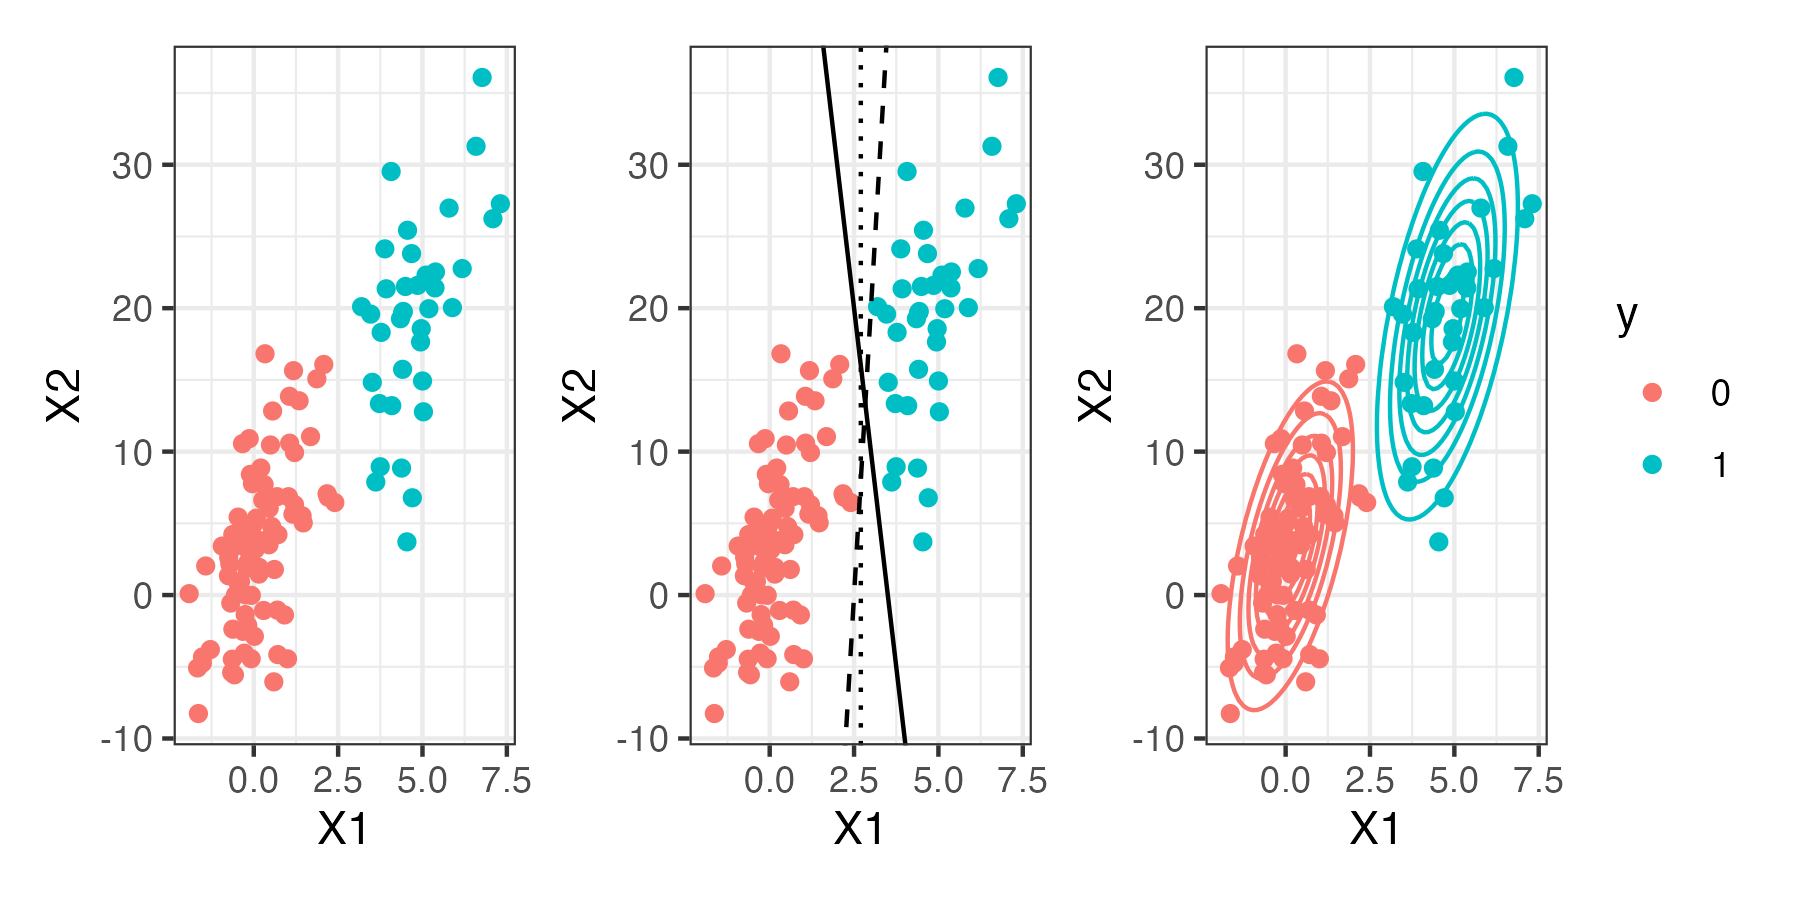
\includegraphics[width=\textwidth]{442_lecs/svm_raw.png}
\caption{A figure to motivate SVMs, and their differences with logistic regression, LDA, or QDA.}
\label{fig_svm}
\end{figure}

What if we want a way to pick between all of the lines in the center panel of Figure~\ref{fig_svm}? And we want a way that does not make a Gaussian assumption?  This is the idea of the maximum margin classifier, which Greta will tell us about in her presentation, and which is summarized in Figure~\ref{fig_svm2}, which is taken from ISL. The idea is quite simple: let's pick between all of the possible separating lines by choosing the one that is as far as possible from all of the training observations. 

\begin{figure}
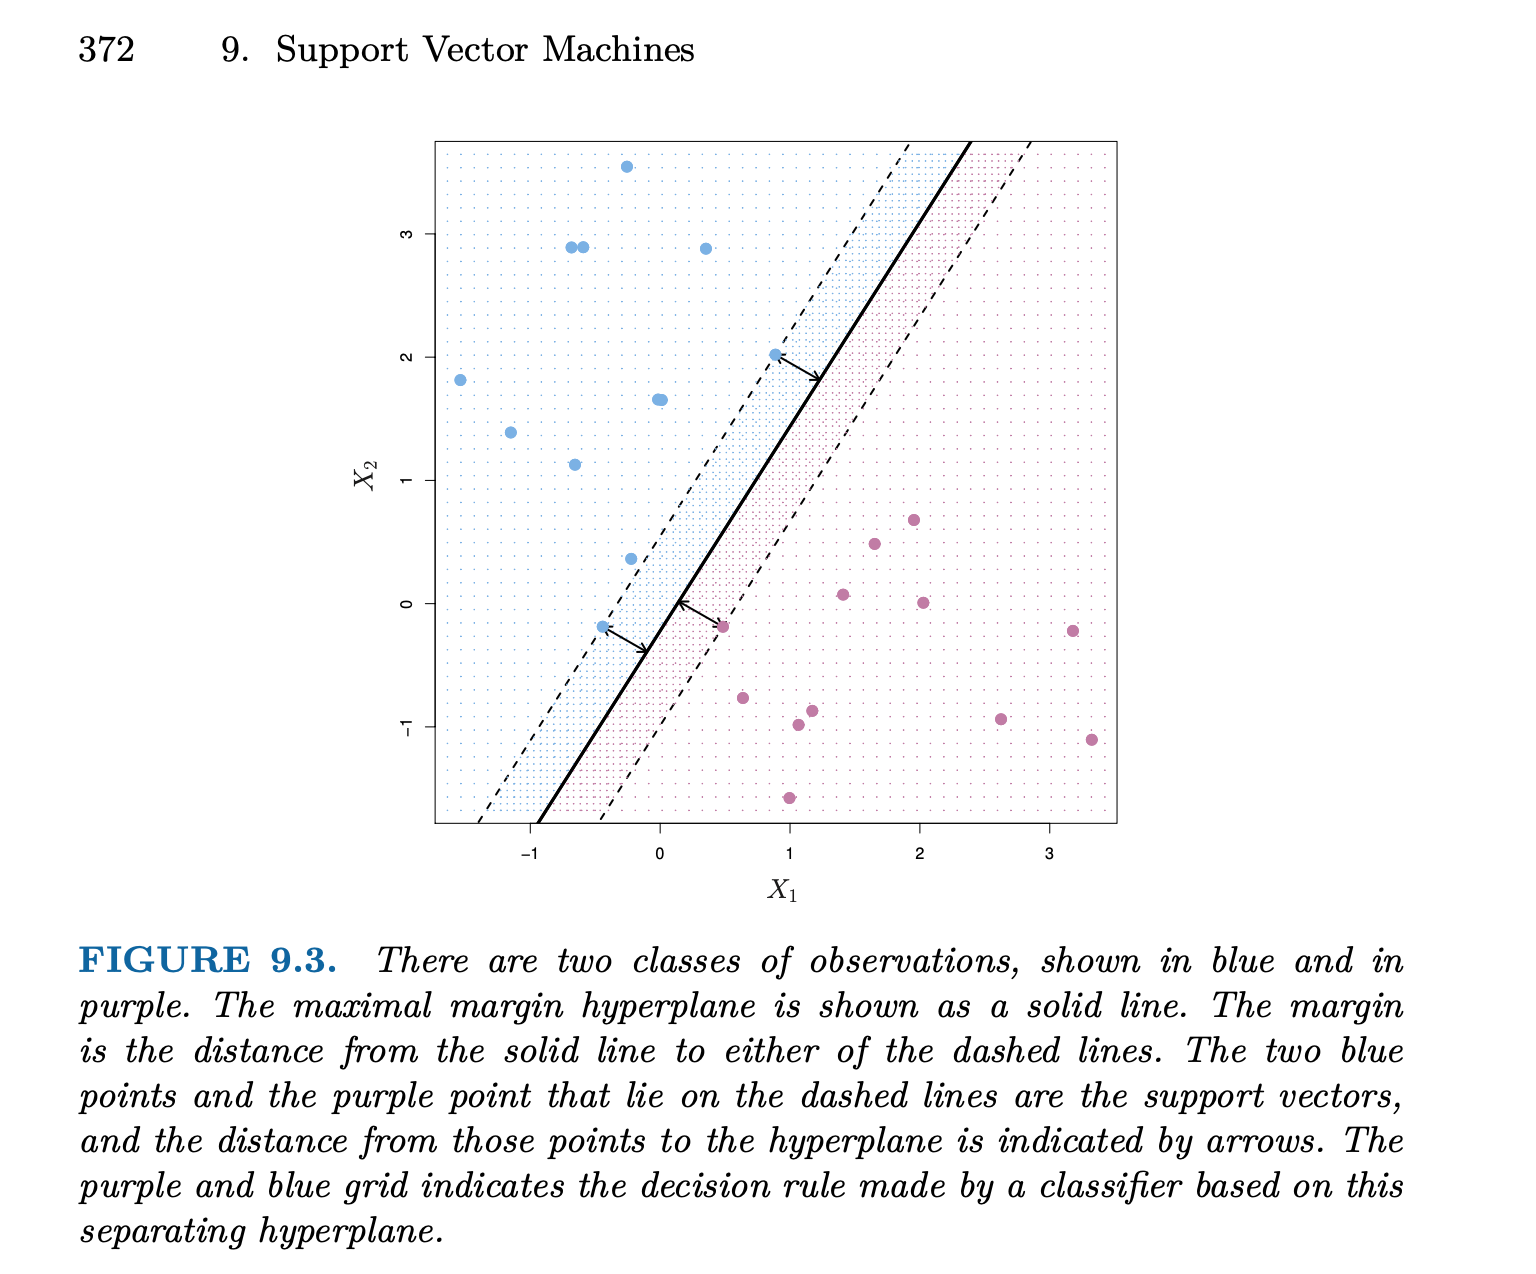
\includegraphics[width=0.8\textwidth]{442_lecs/svm.png}
\caption{The maximum margin classifier picks the line that is far as possible from all observations.}
\label{fig_svm2}
\end{figure}

\subsection{Maximum margin classifier using constrained optimization}

How do we actually fit the line in Figure~\ref{fig_svm2}? There is some math that relates to how we actually draw these lines onto plots. Also, note that we could have more than $2$ $X$ variables, and then we would be using a plane and not a line to separate our classes. 

In general, we will write our linear boundary as the line:
$$
\beta_0 + \beta_1 X_1 + \ldots + \beta_p X_p = 0. 
$$
The idea is to pick a line so that $\beta_0 + \beta_1 X_1 + \ldots + \beta_p X_p < 0$ whenever $y=-1$ and $\beta_0 + \beta_1 X_1 + \ldots + \beta_p X_p > 0$ whenever $y=1$. For today, we are doing binary classification and we are writing our two classes as $-1$ and $1$, for simplicity. 

Any of the lines in the center panel of Figure~\ref{fig_svm} actually have this property. So now the idea is to do even better. Let's both have it be the case that $\beta_0 + \beta_1 X_1 + \ldots + \beta_p X_p < 0$ whenever $y=-1$ and $\beta_0 + \beta_1 X_1 + \ldots + \beta_p X_p > 0$ whenever $y=1$, but also have it be the case that $\beta_0 + \beta_1 X_1 + \ldots + \beta_p X_p$ is basically never TOO close to $0$. Because when it is near $0$, it means that points are close to the line and we have uncertainty. 

%So, the maximum margin classifier says:


\subsection{From maximum margin classifier to support vector machines}



\subsection{Optimization}


\subsection{The kernel trick}


\subsection{What do we think about SVMs?}








\section{Monday, March 17: Catch-up}

Today, we returned to the notes from tree day, since we didn't finish them on tree day. 

\section{Thursday, March 20: Midterm}

In-class midterm, followed by very long spring break. 







\section{Monday, April 7: Model Validation and Selection}

\subsection{Some comments on the midterms}

\subsubsection{Review of common mistakes from in class midterm}
\begin{itemize}
\item \textbf{Problem 2: } Need to mention that deep learning is still subject to the bias-variance tradeoff! For a bit it seemed like double descent was going to challenge this, but recent work has shown that double descent is still governed by the same principles!
\item \textbf{Problem 3:} Recall the difference between a model and a model-fitting-procedure. A linear regression with $5$ covariates is a very simple model. We don't really need to worry about overfitting if we fit linear regression with $5$ pre-specified covariates. But, the procedure of ``search through 16,000 possible covariates and use stepwise regression to select the best $5$" is a very complex model-fitting-procedure. We definitely need to be worried about overfitting in this case! You all saw something really similar to this on a HW problem! 
\begin{itemize}
\item When we talk about bias / variance / overfitting: we are usually talking about a model-fitting-procedure: something that takes in a random training set and outputs a model. On the other hand, when we talk about interpretability or inference (coming soon!), we often want to talk about a specific model. 
\item When we talk about predictive accuracy: which do we care about? This is actually a tricky question, which does not relate to the in-class midterm but does relate to the idea of a ``model" vs. ``model fitting procedure". 
\begin{itemize}
\item If we are getting ready to ``deploy" a specific model to be used in the real world: we probably want to know the predictive accuracy of this specific model: trained on our entire training set! 
\item Unfortunately, this specific accuracy is hard to estimate! We can use cross-validation on the training set to estimate predictive accuracy. But ... this CV uses a bunch of different models fit to different subsets of the training data-- not our full final model! Tricky! 
\item Looking at the predictive accuracy of our fixed model on a large test set would be nice. But ... if we had such a large test, why wouldn't we use some of this data as training data to improve our model??
\end{itemize}	
\end{itemize}
\item \textbf{Problem 4: } In an image classification, the individual pixels are not meaningful! The patterns between the pixels are meaningful. So variable selection and additive models fundamentally don't make much sense. 
\begin{itemize}
\item Consider identical copies of the same image, but in one image everything has been shifted one pixel to the left. Any sort of model that is additive in the original features will be really bad at recognizing these two images as similar! 
\item One implication (relevant to what is coming, not the midterm): we need to think about what we mean by ``interpretable" for an image classification problem. Consider a lasso model that selects 10 pixels to be used for classification. The model is simple enough for us to see what coefficients go with which pixels. But, is it actually useful for us to know the coefficient of pixel (4,17)? How do we make sense of that? 
\end{itemize}
\item \textbf{Problem 5: } Honestly, this went pretty well. There weren't specific rows that everyone got wrong or anything. 
\begin{itemize}
\item One commonly forgotten common principle: if we have a tuning parameter like $\lambda$ in a ridge penalty or $k$ in KNN that directly controls model complexity, we know exactly what changing it will do to training error. Training error is lower for more complex models: it monotonically decreases as we move along the complexity axis! On the other hand, for test error, this tuning parameter has some ``ideal" value that depends on the true data generating mechanism! The test error curve is U-shaped! So we often don't know if it will go up or down as we move along our complexity axis! 
\end{itemize}
\item \textbf{Problem 6: } Check derivative algebra! Also, stochastic gradient descent processes training data in batches, so can be used for online learning. So, we might use stochastic gradient descent instead of the closed form solution for ridge regression if we have so much training data that we don't even want to store it in memory, or if our training data is coming to us over time.
\end{itemize}

\subsubsection{From the takehome midterm}

\begin{itemize}
\item \textbf{Problem 1:} If a proof tells you that something has expected value $c$, and then you simulate to verify your proof, as you increase the number of repetitions, you should be able to get a result that is equal to $c$ with a margin of error of $0.0000001$, and even this should shrink with the number of iterations. 
\begin{itemize}
\item Sometimes the proof will also rely on the sample size $n$ being big or something- and then you will also need to make this big in your simulation. But sometimes it does not! 
\item The empirical average difference between training error and test error should have converged to exactly $2/n p \sigma^2$ as the number of iterations increased. This did not depend on $n$, $p$, or $\sigma^2$.
\item The key thing here that was tricky: the $p$ in the expression is the number of coefficients in your regression model. So, unless you specifically told \texttt{lm()} to remove the intercept, then your effective $p$ is actually $p+1$!
\item If you happened to pick a big value of $n$, then the value of $2/n p \sigma^2$ barely changes when you change $p$ to $p+1$. So this makes this hard to spot. But, for a lot of you, I think the difference was large enough that you should have been able to spot this difference.
\end{itemize}
\item \textbf{Problem 2:} I wanted people to think carefully about exactly what they were seeing, and go beyond what they read in textbook! What the heck was elasticnet doing with those correlated variables? Was it ``good" or ``bad"? 
\item \textbf{Problem 3:} I was happy overall! And, this is basically our topic for today! So, people would do even better after today! 
\end{itemize}

\subsection{Back to regularly scheduled programming: review!}

Before spring break, we learned about so many different machine learning algorithms. We also learned about so many axis on which to compare these algorithms. Let's briefly review these, since it has been a while. This table (while really full) is not at all exhaustive! It's just to remind you of algorithms that we have seen, and some basic properties. You should be able to make a table like this yourself but fill in your own thoughts and ideas!

\begin{table}[H]
\scriptsize
\begin{tabularx}{\textwidth}{|X|X|X|X|X|X|X|}
\hline
&&&&&& \\ 
& When? & Bias? & Variance? & Usability? & Interpretability? & Efficiency? \\ 
&&&&&& \\ 
\hline 
Linear regression (no bells and whistles) & Regression & Unbiased if true model is linear; otherwise likely biased (too simple) & Likely low because simple. Not low if $p$ is really big. & Easy! & Easy! & Easy! \\
\hline 
Linear regression with engineered features (splines, polynomials, etc). & Regression, worried linear isn't good enough.  & Unbiased if you pick good features; otherwise likely biased. & Variance increases if you make engineered features really complicated (splines). Decreases if you are reducing dimension or redundancy (PCA). & Pretty easy, but you need to pick your features (how many PCs, degree of spline, etc). & Not amazing but not a black box. & Pretty good! \\
\hline
Stepwise regression.  & Regression, $p$ is really big, want to select subset.  & Unbiased if true model linear or you added nicely engineered features; biased otherwise. Fewer steps = potentially more bias (miss out on important variables). & Grows if $p$ is bigger or number of steps is bigger. So much greedy searching!& Pretty easy! Need to decide step criteria and stop criteria. & Even better! & Can seem slow, but faster than ``best subset" because greedy approximation.\\
\hline 
Lasso Regression & Regression, $p$ is really big, want to select subset. & Bias grows with $\lambda$, and might just be big if true model not linear. & Variance shrinks with $\lambda$. Never THAT bad if $p$ not too big. & I think easy! Just use CV to tune $\lambda$. & Pretty good! & Pretty good! \\ 
\hline  
Ridge regression  & Regression, $p$ is really big; want to reduce variance.  & Same as lasso. & Same as lasso. & Same as lasso. & Less interpretable than lasso. & Even better than lasso! Closed form! \\
\hline  
Logistic regression; with engineered feature, stepwise, lasso, or ridge extensions & Classification (mostly binary, but has multi-class extensions) & \multicolumn{5}{|c|}{Fill in same as all the linear regression rows.} \\
&& \multicolumn{5}{|c|}{(but now no-bias means that log-odds are linear in the included features).} \\
&& \multicolumn{5}{|c|}{(when classes are well-separated, hard to estimate log-odds in the ``in-between" area. high variance.) } \\
\hline
KNN & Regression OR classification, when you think you have non-linearity, and when $p$ is not too big. & Small if $k$ is small. & Big if $k$ is small. & Easy! Just pick $k$. Not going to work well in high dimensions, and then will need to consider PCA, etc. & Not a black box. ``Prototype" interpretation.  & Can be bad in terms of time and space without clever tricks.  \\ 
\hline 
LDA & Classification, when you think your classes are linearly separable, or, equivalently, Gaussian with shared variance. & Biased if not linearly separable & Pretty low variance. & Easy, I don't even think there is a tuning parameter. & Pretty good! & Easy!  \\
\hline
QDA & Classification when you think your classes are Gaussian with non-equal variance & \multicolumn{5}{|c|}{(Same as LDA basically, just slightly higher variance.)} \\  
\hline 
GAM & Regression. For classification, use logistic GAM. & Low bias because we let our model be really wiggly. But misses out on interactions! & Potentially high variance if we don't regularize or if we have a lot of features & Not bad, but there are a lot of moving pieces we could tweak. & Could be worse. Additive lets us make nice variable-by-variable plots. & Iterative back-fitting required; not bad.   \\
\hline 
Neural Network & Classification or regression; good for complex tasks! & SUPER LOW. Even gets all the interactions & Really high without proper regularization.  & A lot of things to fiddle with; hard to use. & Black-box. & Slow; use stochastic gradient descent.   \\
\hline 
Trees & Classification or regression. & Bias shrinks as tree depth increases. & Variance grows as tree depth increases. & Super easy, although you do need to decide on a stopping criteria, and choice can affect results & Small trees are really easy for humans to interpret. But beware instability! & Fast! \\
\hline 
Support vector machines & Mainly classification! We did not cover the regression setting. & If you use a ``high dimensional" kernel and big budget, really low bias!! & Variance increases as you make kernel higher dimensional or increase budget. & I think pretty easy to use out of the box. & Not that interpretable; I guess you can look at the weights if you are using a linear kernel & A bit slower (you might have noticed this in R!). \\
\hline 
\end{tabularx}
\end{table}

\subsection{No free lunch}

Why is it necessary to introduce so many different statistical learning approaches, rather than just a single best method? There is \emph{no free lunch}\footnote{This is the name of an actual theorem!} in statistics: no one method dominates all others over all possible data sets. On a particular data set, one specific method may work best, but some other method may work better on a different data set. Hence, it is an important task to decide for any given set of data which method produces the best results. Selecting the best approach can be one of the most challenging parts of performing statistical learning in practice.

\subsection{How we pick the best model depends on our goals!}

In the Breiman ``two cultures" reading that you will all complete for Monday, Breiman claims that there are two possible goals of statistical modeling: 
\begin{enumerate}
\item \textbf{Prediction:} Make accurate predictions for new data. 	
\item \textbf{Information:} Describe or understand something about the universe is generating the data.
\end{enumerate}
This probably is not a surprise to any of you- this is a common way to talk about two goals of predictive modeling. In the Efron reading that you will complete for Monday, Efron expands this classical list of two goals to a list with three possible goals. 
\begin{enumerate}
\item \textbf{Prediction:} Make accurate predictions for new data. 
\item \textbf{Estimation:} Learn the parameters of a model that can be written down (e.g. a regression model). 
\item \textbf{Attribution:} Formally determine which variables are important. 
\end{enumerate}
I like that Efron distinguishes between estimation and attribution. However, it is not clear exactly how Efron's three goals map to Breiman's two goals. To gain valuable information, do we need to have parameters that we are estimating? Can we gain information about the universe without doing formal attribution? Also, while I don't think it is a surprise to any of you that we will pick a different modeling approach depending on our ultimate goal, do you think that these different goals are at odds with one another? Or do you think that they can be complimentary? I look forward to hearing what you all think when I read your reading responses next week! 

For the rest of class today, let's assume that our primary goal is prediction. And let's go into a bit more depth about how to select the best model when our goal is predictive accuracy. 


\subsection{A bit more about picking models based on predictive accuracy}

First of all, it is important to note that the \emph{no free lunch} idea applies even if our goal is only predictive accuracy! 

Consider the extremely naive model that ignores the training data and always predicts $\hat{y}=3$. Well, if we happen to live in a universe where $Y = 3 + \epsilon$, and none of the covariates $X$ are important, then this model is optimal in terms of its mean squared error on new data! And the model $\hat{y} = \bar{y}_{train}$ will also do quite well. Since, we never know what the true universe data generating mechanism is, we can never say for sure that this ``intercept-only" model $\hat{y} = \bar{y}_{train}$  is worse than deep learning! 

You all already know that we can't just compare models based on their training error. If we compare models based on their training, then we will always prefer the most complex models with the highest degrees of freedom. In the example above, deep learning will certainly have lower training error than $\hat{y}=3$, because it will fit to the noise in the data. Instead, you all already know that we want to assess which models will perform the best on new, unseen data. 

Let's talk a bit more formally about how we assess expected predictive accuracy on new data. We have already touched on many of these methods/concepts, but I want to close the loop on ESL Chapter 7 because it is such an important chapter!

First, we need to mention that there are two separate things that we might be doing when we try to assess the accuracy of a model on new data. 
\begin{itemize}
\item \textbf{Model Selection:} We want to compare several models or several model-fitting-procedures to decide which one to use as our final model. 
\item \textbf{Model Evaluation:} After choosing a final model, we want to estimate its final accuracy on new, unseen data.
\end{itemize}

Most data analysis pipelines involve model selection. Thus, we usually actually want to do both of these tasks. And, when we are doing both of these tasks, we need to be careful about how we use our data! 

\subsubsection{Train / test / validate}

The gold standard way to carry out a data analysis pipeline that involves both selection and evaluation is the \textbf{train, validate, test} paradigm. The idea is simple. 
\begin{itemize}
\item We split our data into three datasets: train, validate, and test. 
\begin{itemize}
\item To compare a bunch of models, we can train them on the training set, and then we can compute their error on the validation set. We can select the model that seems to perform best on the validation set. 
\item The validation-set error of the selected model is a biased estimate of the true error of this model: we picked it specifically because it was a minimum-- it is biased downwards! 
\item So, we end by evaluating the performance of our selected model on the test set.
\end{itemize}	
\end{itemize}

However, sometimes we don't have enough data to want to split it into three parts! So, there are some other options.

\subsubsection{Fancy equations to estimate test error from training error}

One option! If we can compute or estimate the \textbf{degrees of freedom or optimism} of a model, then we know that the expected test error is related to the training error via a simple formula. Thus, we can use an equation to figure out a \textbf{bound} on the expected test error, and then select the model that seems to have a low expected test error. This eliminates the need for a validation set. This is the reason why we can reasonably select a model based on AIC, BIC, or Mallow's CP. A limitation of these methods is that they relate only to the in-sample (fixed X) prediction error: they say nothing about what might happen at new values of $X$. 

There are a couple of other ways of measuring model complexity besides degrees of freedom or optimism. One is VC dimension! Have any of you heard of VC dimension? This gives you another way to bound the difference between training error and test error. It is a pretty loose bound and we are not going to cover this!

One reason that we don't always use this option: degrees of freedom or VC dimension are very hard to compute for complex procedures!!! So ... we can't actually use these bounds!

\subsubsection{Cross Validation}

Cross validation re-uses data cleverly, and so can be more efficient than a train/test/validate split. But it is also a huge can of worms that is more complicated than it seems.  

First, note that, if we are doing both model selection and estimate predictive accuracy, we really should still separate your data into a training set and a test set. We can then use cross validation on our training set to select a model. We can then re-fit the model with the selected tuning parameter on the entire dataset, and can then evaluate this model on the test set. You have all done this on your HW, basically every time that you have used glmnet: you use \texttt{cv.glmnet} to pick $\lambda$, but you still then evaluated the prediction error on a test set.

One reason that this is important: the CV error of a model that is selected because it minimizes the CV error is biased downward! Because it is a selected minimum! This is a very important concept. 

If we are not doing any selection, and are just doing assessment, then we can get away with doing CV on our entire dataset. But, it is still conceptually tricky to figure out exactly what cross validation error is measuring! Since we fit a different model to each fold, and also each of these models only gets to use $(K-1)/K \times n$ of the data points for training, it is not exactly the same as evaluating the prediction error of a fixed model fit to $n$ observations. When we are just comparing different procedures to select a tuning parameter, we might not care about this. But when we are trying to evaluate a model, we do care! 

Figure 7.8 of ESL, which is copied below as Figure~\ref{fig_cv} shows why the number of folds could have a big impact on what cross validation is actually measuring. Cross-validation as an estimate of expected prediction error has its own bias-variance tradeoff, which depends on the number of folds used. While there is no exact rule for how to decide how many folds to use for cross validation, a good rule of thumb is 5-10.  

\begin{figure}
\centering
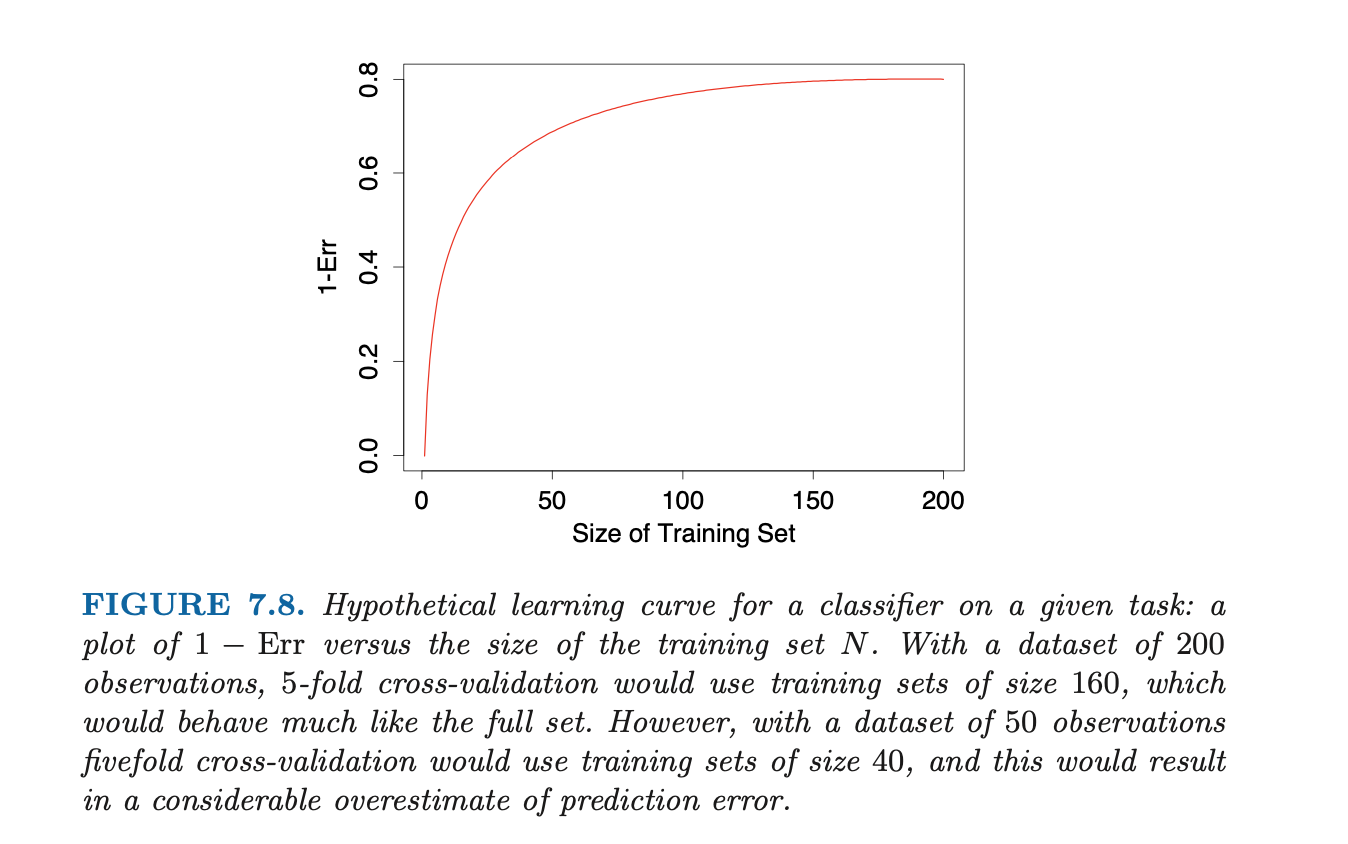
\includegraphics[width=0.6\textwidth]{442_lecs/cv_esl.png}
\caption{Figure 7.8 from ESL!}
\label{fig_cv}	
\end{figure}

You need to be really careful about making sure that model selection and model assessment are both done properly using held out data. Recall your HW problem on the wrong way to do cross validation!! And see ESL 7.10.2. The idea is that we need to use CV to evaluate an entire model-fitting procedure. We are not allowed to do any part of the procedure (i.e. variable selection) using the entire dataset-- if we do, then the test set isn't truly ``held out".

I think that this concludes our study of ESL Chapter 7, and I think you are all experts now at selecting models with good predictive accuracy! Next week, and on your HW, you will think about other things that we might want to consider when selecting a model!











\newpage

\section{Thursday, April 10: Bagging and Random Forests}

\subsection{Model selection recap}

On Monday, we talked about how to select a model if the main thing we care about is predictive accuracy. Roughly speaking, if your main goal is predictive accuracy, then you should be selecting the model with the lowest error on a test set. 
\begin{itemize}
\item You could use a single train/test split. This let's you compare specific models fit to your specific training set.
\item You could use something like 5-fold cross-validation. This makes more efficient use of the data, but you are no longer looking at the error of a specific model fit to the specific training set. You are looking at an average error that results from a model-fitting procedure applied to 80\% of your training set. 
\end{itemize}
There is a lot more that I could say about model selection or about cross-validation. But, at a basic level, you all know how to do this already. You all did it on your take-home midterm, for example. The one thing I want to emphasize that I mentioned briefly last time is the idea of the \textbf{winner's curse.} 
\begin{itemize}
\item Suppose that, in reality, there are three models that are equally good in terms of their expected prediction error over all possible realizations of new test sets. 
\item On the single test set that we observed, one of these models will ``win" due to random chance (i.e. it will have the lowest error on our observed test set).
\item This test error is biased downwards for the expected test error of this model on a NEW test set. Selecting a winner caused us to overfit to our test set. 
\item For an unbiased estimate of a selected model's performance on new, unseen data, we actually need three datasets: train / validation / test. We can select the model that achieves minimum error on the validation set, and only at the end do we evaluate the accuracy on the totally unseen test set. 	
\end{itemize}
The idea of the winner's curse is really important! Selected models tend to let us down in the future :(. Selected policies in government, econ, etc. tend to underperform in the future: they ``won" the first stage of selection partially due to random chance, and now they regress to their mean. This is important to be aware of, any time you are doing model selection!

That's all about model selection for now! If you love model selection, consider a related topic for your final project! 

\subsection{Intro to Ensemble Methods}

Today, let's talk about a totally new and potentially crazy idea: if we only care about predictive accuracy, why do we need to select one model? Why can't we take a bunch of different models that all do pretty well, and average or combine their predictions somehow? 
\begin{itemize}
\item If the different models tend to make mistakes on slightly different types of datapoints, or if their mistakes are uncorrelated with one another, this could really help us! 
\item We need to have room to improve; if we are already achieving essentially irreducible error, then this will not help.	
\end{itemize}
In other words: forget model selection. Let's use an \emph{ensemble model}, that combines the results of several models!

You might be thinking that you are going to fit a KNN, a regression tree, and a lasso regression all to the same dataset, and then average the predictions from all of these different models. We could certainly do that! But, for now, let's not go too crazy with ensemble methods. Let's talk about two relatively simple methods for taking a single model fitting procedure and improving it by fitting it many times in a row. 

\begin{itemize}
\item The general idea of \emph{bagging} is to take one model that has high variance, and reduce the variance by averaging over several repeated copies of this model. We will talk about this today!
\item The general idea of \emph{boosting} is to take one model that has high bias, and reduce the bias by iteratively focusing attention on the examples that we are currently messing up on. We will talk about this next time!
\end{itemize}

\subsection{Bagging (Breiman, 1996)}

Suppose we have a single base learner, such as a single deep decision tree, that we could train to our entire dataset. Call this model $\hat{f}()$. There is a fair amount that we like about a deep decision tree (it can uncover interaction terms, it has low bias). However, there is a thing that we do not like about this decision tree. Due to the high variance of decision trees, we know that if we had observed a very slightly different training set, we would have a totally different tree. This high variance compromises our predictive accuracy! 

Well, here is a really simple idea that works well if we care about predictions. We can take fit $B$ different deep decision trees to $B$ different bootstrap samples of our dataset. Remember that, to get a bootstrap sample, we draw $n$ observations with replacement from our $n$ original training observations. We now have $B$ different prediction models, $\hat{f}_b()$ for $b=1,\ldots,B$: each fit to $n$ observations. We let our final, bagged model (bagging stands for bootstrap aggregation), be:
$$
\hat{f}_{bag}(x) = \frac{1}{B} \sum_{b=1}^B \hat{f}_b(x). 
$$

And that's it! That is the entire idea of bagging!

\subsection{Why does bagging reduce variance?}

We know in statistics that averaging is a nice way of reducing variance. But also, bagging shouldn't be some magical way to make our model really good: taking $B$ bootstrap samples from our data doesn't actually increase the total amount of information in our data! So, what is going on and why does bagging work? 

Let $Var(\hat{f}_{bag}(x))$ be the variance of a prediction for a single fixed test-point $x$. The randomness is taken over the training of $\hat{f}_{bag}()$ for many different training sets. Let $Var(\hat{f}(x)) = \sigma^2$. What is $Var(\hat{f}_{bag}(x))$? 

Well, based on the form of $\hat{f}_{bag}(x)$, we have that:
$$
Var_{bag}\left(\hat{f}(x)\right) = Var\left(\frac{1}{B} \sum_{b=1}^B \hat{f}_b(x) 
\right) = \frac{1}{B^2} \left( \sum_{b=1}^B Var(\hat{f}_b(x)) + \sum_{b=1}^B \sum_{b' != b} Cov(\hat{f}_b(x),\hat{f}_{b'}(x))\right).
$$
Note that, $\hat{f}_b(x)$ and  $\hat{f}_{b'}(x)$ are identically distributed random variables: they both result from applying the same procedure to a random subsample of the same data. Let $Var(\hat{f}_b(x)) = \sigma_b^2$ for any $b=1,\ldots,B$. Also, note that when $n$ is large, $\sigma_b^2$ should be the same as $\sigma^2$: fitting a model to the whole training set should be the same as fitting a model to a bootstrap sample from the whole dataset. Next, note that  $\hat{f}_b(x)$ and  $\hat{f}_{b'}(x)$ are not independent, because they are trained on overlapping subsamples of data. Let $Cov(\hat{f}_b(x),\hat{f}_{b'}(x)) = \rho \sigma_b^2$, where $\rho$ is the correlation induced by the overlapping data. Note that this value is the same for all $b,b'$ from $1$ to $B$. 

So, 
$$
Var\left(\hat{f}_{bag}(x)\right) = \frac{1}{B^2} \left(B \sigma_b^2 + B \times (B-1) \rho \sigma_b^2 \right) = \frac{1}{B^2} \left(B \sigma_b^2 (1 - \rho) + B^2 \rho \sigma_b^2  \right)  = \frac{\sigma_b^2 (1 - \rho)}{B} + \rho \sigma_b^2.
$$

Suppose that we are working with a very stable model fitting procedure. In this case, there probably isn't much change from bootstrap sample to bootstrap sample. This means that there is a lot of correlation between $\hat{f}_b(x)$ and $\hat{f}_{b'}(x)$; $\rho \approx 1$. In this case: 
$$
Var\left(\hat{f}_{bag}(x)\right) \approx \frac{\sigma_b^2 (1 - \rho)}{B} + \rho \sigma_b^2 = \sigma_b^2 \approx \sigma^2. 
$$
Uh oh! This means that bagging did not help us reduce our variance! We did a lot of computational work to get the same variance that we would have had if we had fit just one model to our full dataset. The issue here is the stability-- when we get basically the same model from every bootstrap sample ($\rho \approx 1$), bagging really does not help us!

On the other hand, suppose we have an unstable model, and $\rho$ is positive but less than 1\footnote{Negative $\rho$ would be quite strange, given that the bootstrap samples overlap significantly. I don't think that this would happen.}. In this case, especially if $B$ is large, the variance of our bagged model is smaller than the variance of an individual bootstrap-sample model: $\hat{f}_b(x)$, which is similar in large samples to the variance of our single model applied to the whole dataset: $\hat{f}(x)$. The smaller that $\rho$ is, the better! 

The fact that bagging reduces variance more for unstable models led Breiman, in his original bagging paper, to claim that bagging does not help with linear regression or ridge regression (stable) but helps with stepwise regression or trees (greedy and unstable). This is good to know!

\subsection{Does bagging reduce bias?}

The average of $B$ linear models is still a linear model. Thus, bagging a bunch of linear regressions does not do anything to the expressiveness of our model, and does not impact the bias. On the other hand, consider bagging shallow decision trees (1 split). Each individual tree is so limited in its complexity; but when we combine many together we get a much more complex additive model. One one-level decision tree gets to use only one variable, whereas a bagged ensemble can take into account many variables. In general, the average of $B$ trees cannot necessarily be written as a tree: so we have increased our model space, and therefore may have reduced bias.  

\subsection{Random forests (Breiman, 2001)}

Before 2001, bagged regression trees were already very popular. Trees are a popular learning algorithm; people like that they can uncover interactions without needing to pre-specify them. However, trees are also notoriously unstable. This makes them a prime candidate to benefit from bagging. 

However, in 2001, Breiman combined some existing ideas to make an algorithm that (often) works even better than a bagged ensemble of trees. The idea is simple: we can make the variance reduction of bagging even better by further de-correlating the trees in our ensemble of bagged trees? Or, in other words, by making the individual trees even less stable? 

In random forests, we do exactly this. We add additional randomness to every individual tree in an ensemble of bagged trees.
\begin{itemize}
\item Recall that, to build a CART regression tree, we greedily select the variable and split point that most improves the goodness of fit of our tree right now. We repeat this process recursively; we keep making new splits by picking the best possible variable. 
\item For each individual CART tree in a random forest, we make a small modification. At each split, we only allow ourselves to consider a random selection of $m \leq p$ variables as the possible split variables. Thus, we may not choose the overall best split variable right now; we might need to choose something else if the ``best" variable is not randomly selected. 
\item This makes the individual trees in the forest more different from one another (smaller $\rho$). While it may seem from the derivation above that this \emph{definitely} helps reduce the variance of the bagged ensemble, we need to remember that this also makes   $Var(\hat{f}_b(x)) > Var(\hat{f}(x))$: an individual tree in the forest has extra noise added compared to a single tree fit to all of the data with all of the variables. However, the gain that comes from the de-correlation tends to help.
\item This can also help us with bias. Recall that, due to the greedy nature of a tree, a tree could miss out on potentially important variables or interactions if the greedy process leads it to go down a certain initial path (dominated by one important variable) while missing other paths. Randomization helps the tree explore all paths and find all possible signal or interactions. This can be really helpful- it seems to work really well on real data. 
\item Of course, selecting a small value of $m$ could also be bad for bias. If there are only a few truly important predictors and we select a small value of $m$, for many trees in our forest these important predictors will be left out. This is too bad-- it will cause us to miss out on true signal!
\item In the case of many correlated predictors, a random forests helps us explore different choices of correlated predictors in different trees. This can be helpful. 
\end{itemize}

\subsection{More details about random forests}

\subsubsection{Tuning?}

In a random forest, we need to choose:
\begin{itemize}
\item How many trees $(B)$ should go in the forest?
\item How deep should each tree in the forest be?
\item How many variables $m$ should be considered for each split?	
\end{itemize}

Conventional wisdom says that it is okay to build deep trees (high variance!) inside of the forest, because we do not care about interpretability and because bagging will help us reduce the variance. Conventional wisdom also says that you might as well make $B$ big if your computational power allows you to. Increasing $B$ ``too much" wastes computation, but cannot cause us to overfit, because it does not cause the model to become more complex, it just causes us to converge to an average. We can keep adding trees to the forest until our OOB error (see below) stops improving. 

The hardest variable to tune is $m$. While some ``rule of thumb" out there says to select $m = \sqrt{p}$, there are definitely situations out there for which $m=p$ (no extra randomization) is optimal. The RandomForest package in R has a built-in mechanism for tuning $m$: it seems really important to check this for your dataset. 

\subsubsection{OOB error evaluation}

To tune a random forest, we don't actually need to do cross-validation. This is because there is already some sample-splitting going on during tree-building! 

Each tree in the forest is build to a bootstrap sample of the data. This bootstrap sample tends to have around 2/3 of the observations ``in the bag" and around 1/3 of the observations ``out of the bag". We can compute the MSE for this tree for these ``out of the bag" data points! More generally, for any data-point, we can get a current ``test error" by getting its prediction from the forest using only the trees for which it was out of the bag. This is nice- this MSE is not affected by overfitting. 

We can keep adding trees to our forest until the OOB error stops improving. This will be when we have more trees than necessary: since the OOB MSE doesn't get to use as many trees per datapoint to get predictions as we would use for new data. But its still a useful metric that can tell us when we clearly don't need more trees. 

\subsubsection{Permutation importance}

While random forests provide a clear way to improve on the predictive accuracy of a single tree, they also lose one of the main benefits of trees: interpretability. However, as we discussed, should we really call an unstable model (a single tree) interpretable? If you would like to use a random forest but would also like to know about which variables are important to your model, people have developed a variety of simple \emph{explainability} techniques that try to get at this. One of them is permutation importance, which is built into the random forest R package. We will cover this next Thursday, on interpretability/explainability day!


\subsection{A discussion: let's go back to no-free-lunch}

Varya was working on an RDemo for you all that was supposed to show that a random forest outperformed bagging! However, with either simulated data or fairly simple real datasets, she was having trouble showing this result! Often, bagging (use all features) was still beating random forests! After looking through her code and trying to debug it (there were no bugs), I came to some conclusions. 

\begin{itemize}
\item Just because your textbook says that random forests should outperform bagging doesn't mean they will on simple datasets: there is no free lunch! No algorithm outperforms all other algorithms on all datasets! 
\item For the randomization idea to be useful, there needs to be ``room for improvement". For example, if your data has tricky-to-find effects with lots of important variables, then the extra randomization might really diversify the trees in your forest and really help. Real datasets tend to be super complex, which is likely why people claim random forests work so well in the real world. 
\item When your data is not super complex, you probably want $m=p$. Setting $m < p$ makes the bias and variance worse for every individual tree: so unless you are really gaining something from this when you average, you probably don't want to do it!
\item In practice, since there is no free lunch, it is always important to tune your models! Nothing is REALLY ``off the shelf". 
\item Don't just blindly trust what a textbook says! Everything depends on your data!
\end{itemize}






\section{Monday, April 14: Boosting}

The entire idea of 
\section{Thursday, April 17: Explainability vs. Interpretability!}

We are going to spend some time today covering the boosting content that we missed. We are also going to have a short discussion of the ``two cultures" reading. Thus, we won't have time to cover too much new content today. 

For the last few classes, we have thrown interpretation to the wind. We have talked about selecting models based on predictive accuracy, and we have talked about ensembles, which are certainly hard to interpret. We have been imagining for the last few classes that our primary goal is predictive accuracy.

Today, let's assume that our primary goal is to learn something about the world. We don't need to make predictions for a new, unseen dataset. We need to understand the data that is in front of us! There are actually two ways that we could accomplish this goal. 

\begin{itemize}
\item We can fit an \textbf{interpretable} model, otherwise known as a \emph{glass box}. Examples include simple or sparse linear models, or small decision trees. With these models, we know exactly what variables are playing a role in our predictions, which presumably helps us understand the world.
\item We can fit a \emph{black-box} model, but then \textbf{explain} this model after the fact using a separate algorithm. This is the huge and growing field known as explainable AI. The only example we have mentioned so far of an explainability technique is permutation importance for random forests (this was also in your Breiman reading). But we haven't yet done this topic justice!
\end{itemize}

Today, I want to just briefly touch on possible explainability techniques for determining important variables. They are both very simple, and pretty general-purpose with a lot of room for tweaks. There are many versions of these out there: I am presenting really simple versions. We will use this just to have a language for discussing interpretability vs. explainability! 

\subsection{Permutation importance (no retraining)}

The idea is to figure out what variables are most contributing to your predictions in a given black-box model.

\begin{itemize}
\item Fit a model $\hat{f}()$ to predict $y$ using a training set. Measure the loss on a test set: i.e. compare $\hat{f}(x^{test})$ and $y^{test}$.
\item For variables $j=1,\ldots,p$:
\begin{itemize}
\item Randomly permute the values of variable $j$ in the test set to get $\tilde{x}^{test}$.
\item Measure the loss between $\hat{f}(\tilde{x}^{test})$ and $y^{test}$. 
\item The increase in loss from permuting the $j$th variable is the importance of the $j$th variable. 
\end{itemize}
\end{itemize}

This idea is really simple, and is effective in telling us which variables are contributing to our predictions. But, it has a lot of problems if we try to interpret it as a measure of the association between variable $j$ and $y$.

Imagine that $x_j$ and $x_k$ are extremely highly correlated, and both associated with $y$. But imagine that our model decides to only use $x_k$ for its predictions. Well, then according to permutation importance, $x_j$ is not important at all. But that doesn't mean it is not associated with $y$- it is just being masked by $x_k$. 

So ... this leaves something to be desired. Note that glass-box models have this issue too though: this just means that attribution is really hard, not that permutation importance has this unique failing.


\subsection{Leave one out importance (with retraining)}

This one is actually even more strange! The idea is subtly different, and this is much more computationally expensive than the idea above.

\begin{itemize}
\item Fit a model $\hat{f}()$ to predict $y$ using a training set. Measure the loss on a test set: i.e. compare $\hat{f}(x^{test})$ and $y^{test}$.
\item For variables $j=1,\ldots,p$:
\begin{itemize}
\item Leave variable $j$ out of the training set to get $x^{train}_{-j}$.
\item Refit the model on the training set. Now you have $\hat{f}_{-j}()$. 
\item Measure the loss between $\hat{{f}}_{-j}({x}^{test}_{-j})$ and $y^{test}$. 
\item The increase in loss from removing the $j$th variable is the importance of the $j$th variable. 
\end{itemize}
\end{itemize}

In some ways, this feels more thorough to me. But in the case where $x_j$ and $x_k$ are extremely highly correlated, and both associated with $y$, I think we get even worse results. In the previous example, at least $x_k$ would have popped up as important. Here, when $j$ is left out, $k$ can absorb its effect. But when $k$ is left out, $j$ can absorb its effect. So we might end up reporting neither of these as important! This is not desirable! 

This again is something that can happen in interpretable models too! If we include $x_j$ and $x_k$ both in a regression in this setting, the variance inflation factors that come from their correlation could lead us to report neither as significant. 

\subsection{Model distillation (student/teacher methods)}

(fill in)


\subsection{Other explainability methods?}

There are many other methods that Lucy or our guest speaker next week might tell us about! And I will try to post some additional readings! This could probably be an entire class, so it was hard to know what to focus on!



\subsection{Do we want interpretability? Or is explainability enough?}

\subsubsection{Some arguments for interpretability}

See Rudin paper. 

\subsubsection{Some arguments for explainability}

Breiman strongly makes the point that models that are simple enough to be interpretable are often less accurate. He says that this is bad, because we only want to learn about the world from a model that is accurate enough to explain the world. I actually have some sympathy for this viewpoint: can we really learn something trustworthy about the world from a model with really low predictive accuracy? I am not sure! The economists would say yes!

A point that I take more seriously is the point about stability. We love trees because they are supposedly interpretable. But, we also know that a tiny perturbation to a training set could cause a tree to look totally different and have totally different variables at the topmost splits. Should we really be interpreting something so unstable? With this in mind, fitting many trees to bagged samples and recording which variables get selected over and over again suddenly seems a lot more appealing as a measure of variable importance.

Overall, we like that we can see into glass boxes. But, if the glass boxes don't work well or are not stable, why do we care? I think these are reasonable points!

\subsubsection{More coming!}

I will put a reading on HW7 where you read about someone who really thinks we ought to be using interpretable models, not explaining black boxes. But also, in your guest lecture next Thursday, you will learn a bit more about explainability! So these topics are not going away, this is just your intro!




\section{Thursday, April 17: Interpretability}

We have been talking for weeks about how interpretability is something that we value! Why? Because if we are going to make sure that our model doesn't do something super unexpected or unfair in real world applications, we probably want to know what is happening inside of the model. Where are the predictions coming from? 

Okay, but what do we actually MEAN by interpretable? prevent oversummarization and can
highlight details for follow-up study. Similarly, an interpretable model can be broken down into
relevant components, each of which can be assigned meaning. Instead of information density
(showing more of the data), interpretability relies on faithfulness (showing more of the model).


nterpretability must be tailored
to an audience and the problems they need solved (Lipton, 2018). There are different levels of
data literacy, and visual representations may be familiar to some audiences but not others.support the transition from automated to augmented decision-making (Heer, 2019), enhancing
rather than substituting human reason. I LOVE THIS POINT. 

NO BLANKET STATEMENTS ARE POSSIBLE. discussions of interpretability can go beyond dichotomies about models being either glass or black
boxes.

\textbf{One thing we should talk about today: Interpretable vs. Explainable.}

INTERPRETABLE. Sparse linear model. Glass Box. 

EXPLAINABLE: something like a partial 

 First,
consider intrinsically interpretable models. When we call a linear model interpretable, we are
invoking parsimony and simulatability. Parsimony means that predictions can be traced back to
a few model components, each of which comes with a simple story attached. For example, sparse
linear models have few nonzero coefficients, and the relationship between each coefficient and the
output can be concisely described. A similar principle applies to generalized additive modeling,
which have few allowable interactions (Caruana et al., 2015), or in latent variable models, which
have few underlying factors (Sankaran and Holmes, 2023). Simulatability formalizes the idea that
predictions can be manually reconstructed from model descriptions. For example, in decision trees
and falling rules lists, this can be done by answering a sequence of yes-no questions. Finally, since
interpretation requires human interaction, it can be affected by the gulfs of interaction (Hutchins
et al., 1985). Ideally, an interpretability method should allow users to quickly query properties
of the underlying model. Further, the method’s outputs should be immediately relevant to the
query, requiring no further cognitive processing. To the extent that a method has reached these
two ideals, it has reduced the gulfs of execution and evaluation, respectivel


BUT.. its not so simple. A lineart model is interpretable only if sparse. A ndecision tree is interpretable only if small. 

LOCAL vs. GLOBAL. KNN has a LOCAL interprettation. Here is why YOUR prediction got made. But nothing global. Global = overall affect of a variable. 

Sensitivity: what happens when I tweak this? 

We can often learn salient, non-obvious characteristics of the data by applying a intrinsically
interpretable model. Some have argued that with sufficient ingenuity, such models can rival the
accuracy and efficiency of any black box (Rudin, 2019). Even otherwise, the results of intrinsically
interpretable analyses can guide the application of more sophisticated models later on.


Sparse and tree-based models are the foundation for many proposals for interpretable machine
learning (Xin et al., 2022; Zhong et al., 2023). 

For example, Zeng et al. (2016) introduced fast
decision trees that match black box models in recidivism prediction, a domain with significant
moral ramifications where interpretability is crucial. Similarly, Hazimeh et al. (2020) designed a
decision tree variant that competes effectively with deep learning in various operations research
tasks. By leveraging advances in combinatorial optimization, their approach allows interpretable
trees to be learned from very large datasets without excessive compute demands

The parsimony of these estimates aligns with our discussion of the characteristics of intrinsically interpretable models. In both approaches, prediction relies only on a small subset of the
original inputs. But how much can we trust these features? Fig 2e - f shows the estimated βˆ
for nonzero features obtained from separately fitting the sparse logistic regression approaches
on independent splits. When using concatenated inputs, only two features overlap, while with
summary statistics, this increases to 18. Therefore, while the model on raw time points may be
more parsimonious, it is less stable.
\section{Monday, April 21: Inference}

Inference = confidence intervals and p-values. Quantify uncertainty. This is, in my opinion, the total real key of statistics. For today, suppose we care about confidence intervals. 

Remember that in linear regression we could have con








\end{document} 















